\documentclass[11pt, letterpaper]{extarticle} % Allows more customization (compared to 'article')
\usepackage[top=1in, bottom=1in, left=1in, right=1in]{geometry} % Specify 1in margins
\usepackage{hyperref} % Used for creating links to sections, equations, external links
\usepackage{cprotect}
\usepackage{graphicx} % Required for inserting images
\usepackage{subfig} % Used for having multiple subfigures within one figure
\graphicspath{ {./figures/} }
\usepackage{rotating} % Used to create sideways figure
\usepackage{amsmath} % Extended math equation functionality
\usepackage{amssymb} % More math notation (e.g., therefore, etc.)
\usepackage{lipsum} % For placeholder text
\usepackage[font=small,labelfont=bf, width=\textwidth]{caption} % custom caption settings
\usepackage{titling} % Custom title page
\usepackage{setspace} % Allows control of double/single spacing
\usepackage[sortcites=true]{biblatex} % Creates the references, makes sure in-line citations are in numerical order
\addbibresource{refs.bib}

\title{Bubble Localization and Rendering for the SBC}
\author{Mahebub Aalam Khatri}
\date{August 2024}

\begin{document}

% \maketitle
\begin{titlingpage} %This starts the title page
\begin{center}

\includegraphics[width=0.5\linewidth]{nucs_logo.png}\\ %Put the logo you want here
\begin{Large}
    \vspace{0.5in}
    \textbf{Technical Report}\\
    \textbf{Number: NU-CS-2024-17}\\
    \vspace{0.1in}
    \thedate\\
\end{Large}
\vspace{0.5in} %You can control the vertical distance
\begin{Large} 
    \textbf{\thetitle} \\
    \theauthor\\
\end{Large}
\end{center}

\vspace{0.2cm}

\centerline{\textbf{Abstract}}
\hspace{0.1\parindent} This paper discusses the methods and challenges involved in localizing the 3D positions of bubbles in the SBC collaboration's scintillating bubble chambers, tests those methods by creating photo-realistic renders of the chambers using Mitsuba, and discusses the factors that most influence the localization errors. The accuracy of 3D localizations is found to depend primarily on the error in the the ray origins and directions used in triangulation. Consequently, factors which impact the triangulation rays have the biggest effect on errors. Those factors in order of their sensitivity to triangulation errors are: camera pose, distortion mapping (e.g., accounting for distortions in the images caused by the camera lenses and refractive surfaces within the chambers), and 2D pixel localization of bubbles in the images. Errors in pixel localization and camera pose are found to have a linear relationship with the triangulation error. Distortion mapping functions fit with incorrect indices of refraction for the fluids in the chambers were also found to cause a linear relationship with the triangulation error as a function of the errors in the indices of refraction. Optimization methods that minimize reprojection errors are shown to have little impact on improving the accuracy of 3D localization. The related code and files for this paper can be accessed here: \cprotect{\href{https://github.com/MA-Khatri/BubbleLocalizationAndRendering}}{\verb|https://github.com/MA-Khatri/BubbleLocalizationAndRendering|}.

\vspace{1cm}

\centering
\textbf{Keywords}\\
Computer vision, rendering, triangulation, optimization 

\end{titlingpage}

\newpage
\tableofcontents
\newpage

% \doublespacing

\section{Introduction} \label{sec:introduction}
The Scintillating Bubble Collaboration (SBC) is developing liquid-noble bubble chambers capable of detecting sub-keV nuclear recoils. These chambers will enable the search for GeV-scale dark matter (DM) candidates called Weakly Interacting Massive Particles (WIMPs) and provide precise measurements of the coherent elastic neutrino-nucleus scattering (CE$\nu$NS) cross section which can give hints for a solution to the matter/anti-matter asymmetry \cite{alfonso2023scintillating, alfonso2022snowmass}. The SBC's first physics-scale device, a 10-kg liquid argon bubble chamber ``SBC-LAr10," is currently being commissioned at Fermilab to calibrate background discrimination power and sensitivity to nuclear recoils at energies down to 100 eV, along with a functionally near-identical clone being constructed at SNOLAB (``SBC-SNOLAB") with a focus on radiopure construction which is projected to achieve the desired sensitivity for detecting dark matter-nucleon scattering. 

These chambers feature a target fluid of superheated liquid argon which, in the rare case of a dark-matter interaction, creates a burst of ultra-violet scintillation light and a bubble. To capture this event, SBC-LAr10 uses a combination of silicon photo-multipliers (SiPMs) which capture the initial burst of scintillation light, piezo-electric acoustic sensors which measure the pressure waves created when a bubble forms, and a ring of three forward-illuminated cameras which look down the chamber and capture images of the bubbles as they form and grow in the target fluid. See figure \ref{fig:chamber_schematic} for a visual breakdown of the chamber and its sensors. This paper focuses on the camera system and how it can be used to detect and localize bubbles within the chamber while accounting for a variety of distortions in the images. For a more in-depth review of the SBC's science objectives and operational details, we direct the reader to the SBC white paper \cite{alfonso2022snowmass}. 

\begin{figure}[h]
    \centering
    \subfloat[Schematic]{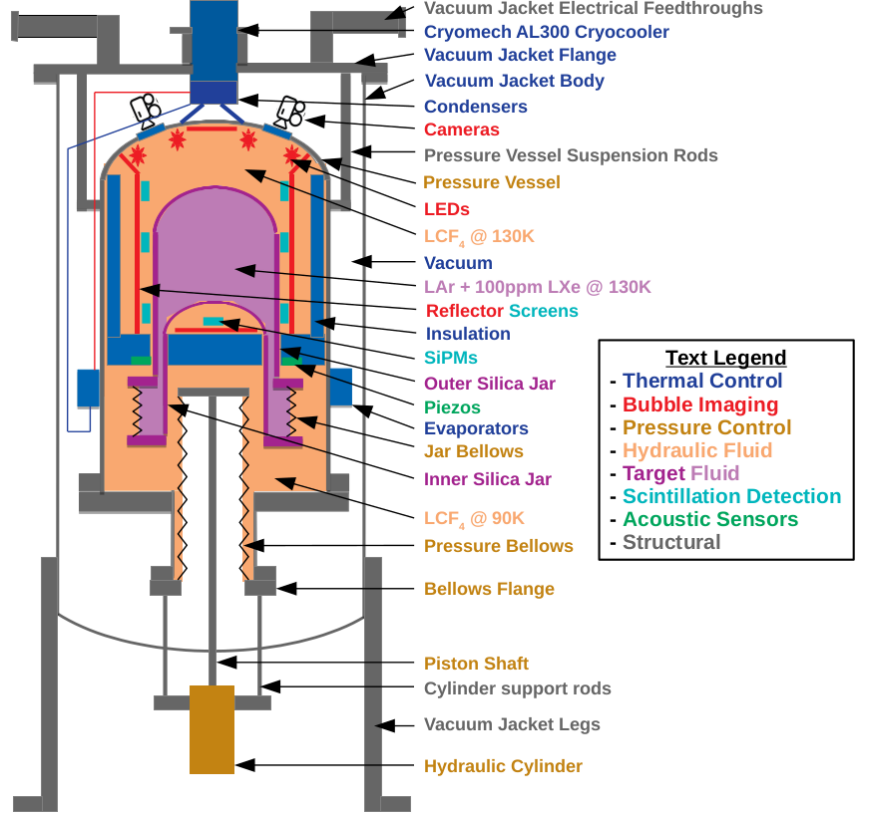
\includegraphics[height=2.8in]{annotated_schematic.png}}
    \hfill
    \subfloat[Solid Model]{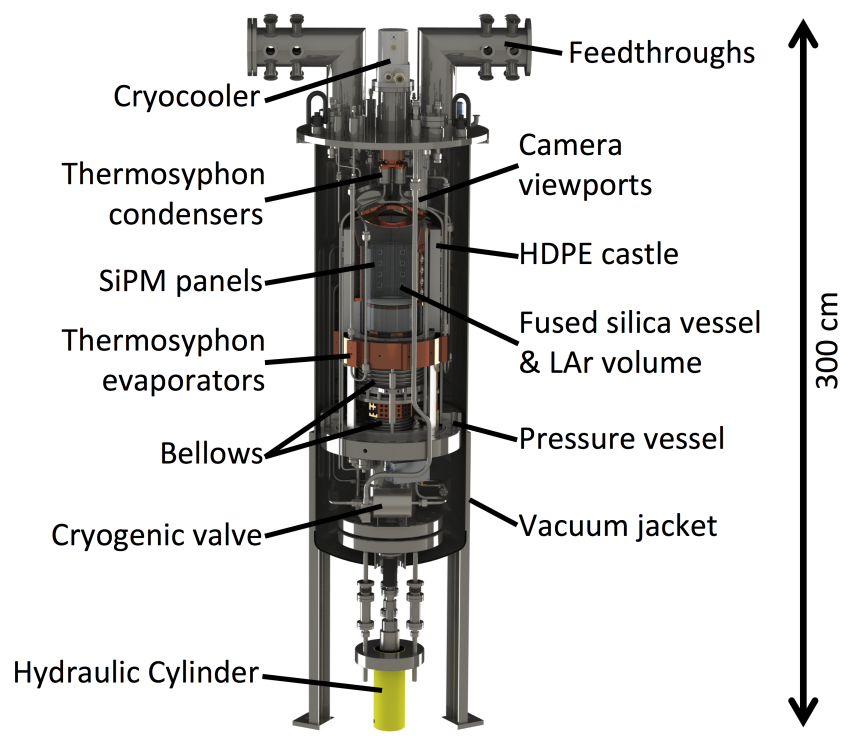
\includegraphics[height=2.8in]{annotated_solid_model.png}}
    \caption{Annotated schematic and solid models of SBC-LAr10. The bubbles to be imaged will form in the liquid argon (LAr) inter-jar volume (purple region of the schematic). The cameras are within the vacuum jacket, looking down through three viewports into the inner pressure vessel. Figures courtesy of \cite{alfonso2022snowmass, alfonso2023scintillating}.}
    \label{fig:chamber_schematic}
\end{figure}

\subsection{The SBC-LAr10 Camera System} \label{subsec:the_sbc-lar10_camera_system}
% While the sensors work in a vacuum, tests have shown that they do not operate at the cryogenic temperatures used in the chamber. Therefore, the sensors are displaced 17 cm from the primary fish eye lens using a series of relay lenses (see figure 9 in \cite{alfonso2022snowmass}) which have the additional benefit of reducing the radiopurity constraints on the SBC-SNOLAB chamber. This relay lens system retains most of the field of view of the fish eye lenses but may cause the image to be slightly out of focus. In this paper, we ignore the relay lens system and make the assumption that the sensor is right next to the primary fish-eye lens to simplify calculations. This assumption is valid assuming the primary visual artefacts introduced by the relay lens system is a slight blur and a small, calculable change in the field of view.
The camera system of SBC-LAr10 consists of three Arduino OV9281, 1 megapixel, global shutter, monochrome camera sensors with a resolution of 1280 by 800 pixels. Each of the cameras' fish-eye lenses look down through a sapphire viewport into the chamber. The chamber itself is illuminated using rings of 850 nm LEDs attached to the interiors of each of the viewports. The LED rings are pulsed concurrently with the camera exposures and have a 10\% duty cycle, allowing the chamber to be dark for 90\% of the time to allow for the detection of scintillation light. The cameras capture images at 100 frames per second, expected to capture 100 ms before and after bubble nucleation \cite{alfonso2022snowmass}. The chamber itself is lined with reflective PTFE to provide better contrast for the bubble images.

Within the field of view of each of the cameras are 5 fiducial markers suspended with wire whose exact positions are known with sub-millimeter accuracy. These fiducial markers are used to determine the camera pose matrices which encode the cameras' positions and rotations (see \S\ref{sec:estimating_camera_parameters}). In this paper, the origin of the world coordinates is set to be the central fiducial marker with the jars along the $-z$ axis (placing the cameras themselves along $+z$).

\subsection{Bubble Localization and its Challenges} \label{subsec:bubble_localization_and_its_challenges}
At a basic level, to localize a bubble in 3D space, we can shoot a ray from each camera in the direction of the bubble in its image and find the point of closest intersection of each of those rays. However, the process to accurately determine the origin and the direction that each ray should travel involves several steps and even after rays have been cast and an initial guess for the bubble location has been created, optimizations can be performed to improve the estimate. This section will introduce the steps involved in bubble localization which will be expanded upon in later sections. 
 
 To localize a bubble, we first need to determine the initial \textit{distorted} pixel location of a bubble in each cameras' image. If there is more than one bubble in each image, we also need to determine which bubble locations correspond to each other across the images. Strategies for initial bubble detection and matching are discussed in \S\ref{sec:bubble_detection}. 

Next, we need to undistort the pixel positions in order to accurately determine the direction that triangulation rays should be fired. The images from each camera are distorted by a number of refractive elements that lie between the sensor and the bubble. The sources of distortion for an outgoing ray from the sensor are, in order: 
% The first distortive elements are the relay lenses which help distance the sensor from the viewports. However, these relay lenses are ignored in this paper since they should not significantly impact the images, only serving to transfer the image farther back from the viewports. Therefore, we assume the sensor is located at the usual focal length of the primary lens. Then, the remaining sources of distortion for an outgoing ray are, in order:
\begin{enumerate}
    \item Barrel distortion introduced by the fish eye lenses themselves.
    \item Magnification caused by looking through the viewports into a medium with a higher index of refraction (IoR).
    \item Distortions caused by the curved jar surfaces and changing IoRs with further distortion introduced by waviness in the jar surfaces due to their manufacturing process.
\end{enumerate}
Techniques for handling each of these distortions are discussed in \S\ref{sec:dealing_with_distortions}.

We also need to know the intrinsic and extrinsic parameters of the cameras. The intrinsic parameters are represented by the \textit{camera matrix} $K \in \mathbb{R}^{3 \times 3}$ encoding the camera's focal center in pixels ($c_x, c_y$) and scaling factors along the $u, v$ axes of the image coordinates from the camera coordinates ($f_x, f_y$). The camera matrix is what converts a point from the camera coordinate system where points are projected onto a plane with bounds $[-1, 1]$ along the camera's local $x, y$ axes (assuming the point is within the field of view of the camera), to the image coordinate system where points are represented in pixel coordinates along its $u, v$ axes. The \textit{extrinsic matrix} (or \textit{pose matrix}\footnote{The extrinsic matrix or pose matrix as described here is similar to the \textit{view matrix} in computer graphics. However, the view matrix is instead represented by a $\mathbb{R}^{4 \times 4}$ matrix where the bottom row is $[0,0,0,1]$ to make matrix multiplication easier. For the simulations, the view matrix is used to determine the pose matrix by simply removing the last row. Note however, that in Mitsuba, the view matrix of the sensor is represented by the sensor's \textit{to\_world} matrix.}) $V \in \mathbb{R}^{3 \times 4}$ is composed of a rotation matrix $R \in \mathbb{R}^{3 \times 3}$ and a translation vector $\mathbf{t} \in \mathbb{R}^{3}$. Together, the extrinsic and intrinsic camera matrices take a homogeneous point in world space ($\mathbf{w}^h \in \mathbb{R}^{4}$) and project it first into camera space and then to image space with homogeneous pixel coordinates ($\mathbf{p}^h \in \mathbb{R}^{3}$). See equation \ref{eq:camera_intrinsic_extrinsic}. The methods for estimating these parameters are discussed in \S\ref{sec:estimating_camera_parameters}.

\begin{align} 
    \label{eq:camera_intrinsic_extrinsic}
    \mathbf{p}^h &= K V \mathbf{w}^h = K [R|\mathbf{t}] \mathbf{w}^h \\
    \label{eq:camera_intrinsic_extrinsic_expanded}
    \begin{bmatrix} 
        u \\ v \\ 1 
    \end{bmatrix}     
    &= 
    \begin{bmatrix}
        f_x & 0 & c_x \\
        0 & f_y & c_y \\
        0 & 0 & 1
    \end{bmatrix}
    \left[ 
    \begin{array}{@{}ccc|c@{}}
        r_{11} & r_{12} & r_{13} & t_1 \\
        r_{21} & r_{22} & r_{23} & t_2 \\
        r_{31} & r_{32} & r_{33} & t_3
    \end{array}
    \right]
    \begin{bmatrix} 
        x \\ y \\ z \\ 1
    \end{bmatrix}
\end{align}

Once we know the camera and pose matrices for each of the cameras, we can use them to generate our outgoing rays in the direction of the undistorted pixel positions of the bubbles in each of the images. Starting with the pixel positions, we can convert them into normalized image coordinates by multiplying the homogeneous pixel positions by the inverse of the camera matrices. Then, the ray origin ($\mathbf{O}_{\text{ray}}$) will be the translation vector of the pose matrix (i.e., the position of the camera) and the ray direction ($\mathbf{d}_{\text{ray}}$) will be the normalized image coordinate multiplied by the rotation matrix component of the pose matrix.
\begin{align}
    \label{eq:ray_origin}    \mathbf{O}_{\text{ray}} &= \mathbf{t} \\
    \label{eq:ray_direction} \mathbf{d}_{\text{ray}} &= R K^{-1}\mathbf{p}^h
\end{align}

After determining the ray origin and direction for the corresponding bubble location in each of the cameras, we can triangulate the real-world location of the bubble using one of the methods described in \S\ref{sec:bubble_triangulation}. Those triangulation methods can give us a good initial estimate of the bubble position. However, it is possible to slightly improve the result by optimizing over the sum of reprojection errors using one of the methods described in \S\ref{sec:optimization_techniques}. Though, it should be noted that in this particular application, the optimizations seem to have a minimal effect on improving triangulation accuracy.

% \subsection{Testing in Simulation} \label{subsec:testing_in_simulation}
% All of the bubble detection, distortion mapping, and triangulation algorithms presented in this paper were tested by creating simulated images of the chamber using the research-oriented renderer \textit{Mitsuba 3} \cite{jakob2022mitsuba3}. An in-depth discussion of how the renders were set up and how future users can manipulate and adjust the rendering parameters to run their own simulations can be found in \S\ref{subsec:setting_up_the_scene_to_render_in_mitsuba}.


\section{Rendering the Bubble Chamber} \label{sec:rendering_the_bubble_chamber}
All of the bubble detection, distortion mapping, and triangulation algorithms presented in this paper were tested by creating simulated images of the chamber like those in figure \ref{fig:real_and_rendered_images} using the research-oriented renderer \textit{Mitsuba 3} \cite{jakob2022mitsuba3}. These renders were made possible due to pre-existing CAD models of the chamber which were converted into polygon files, cleaned up, segmented, and restructured using Blender, then assigned materials in Mitsuba and rendered. \S\ref{subsec:setting_up_the_scene_to_render_in_mitsuba} goes into the details of converting the CAD models into renderable scenes in Mitsuba. \S\ref{subsec:testing_setup} discusses the basics of the setup used for testing and bench-marking the remapping, triangulation and optimization algorithms covered in later chapters. Meanwhile, \S\ref{subsec:path_tracing} briefly discusses the theoretical foundations of \textit{path tracing}, the rendering pipeline used in creating the simulated images with Mitsuba, as well as its relevant limitations.

\begin{figure}[h]
    \centering
    \subfloat[]{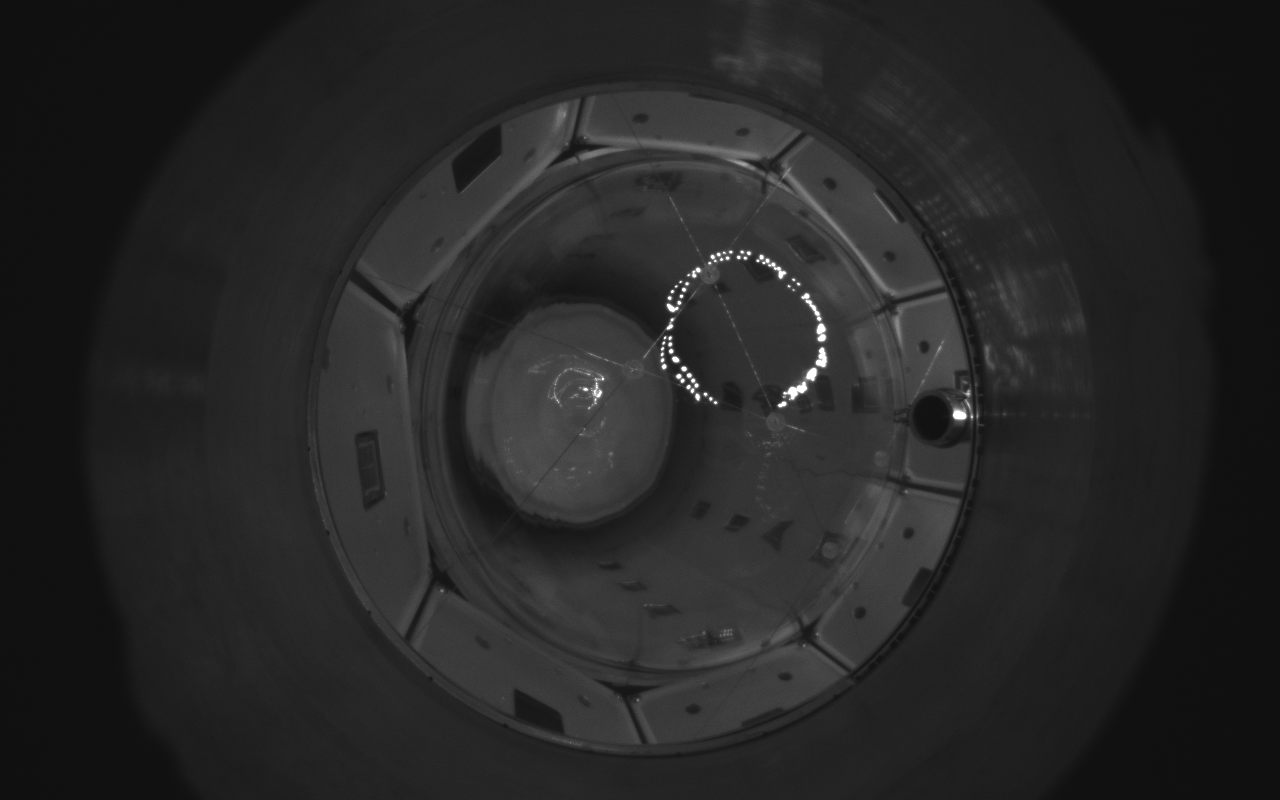
\includegraphics[width=0.33\textwidth]{led1-cam2.png}}
    \hfill
    \subfloat[]{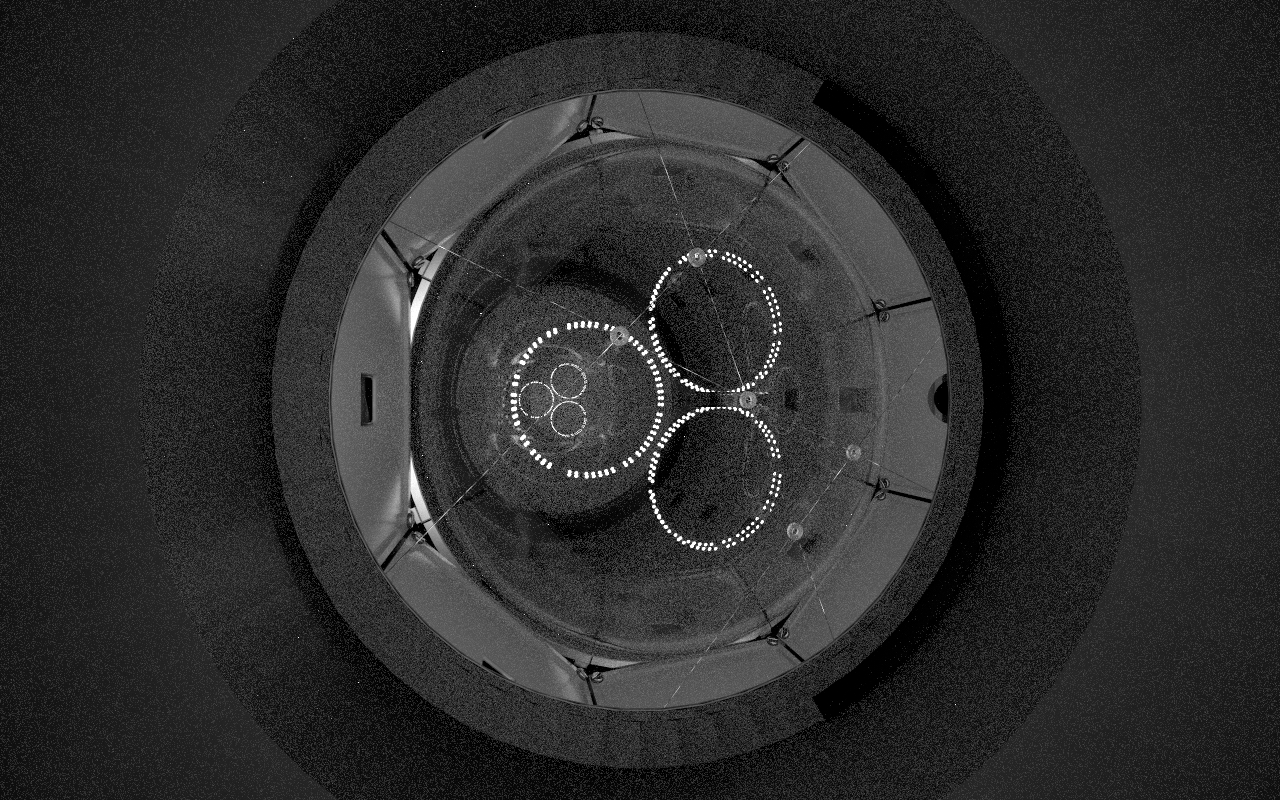
\includegraphics[width=0.33\textwidth]{render_no_fluid.png}}
    \hfill
    \subfloat[]{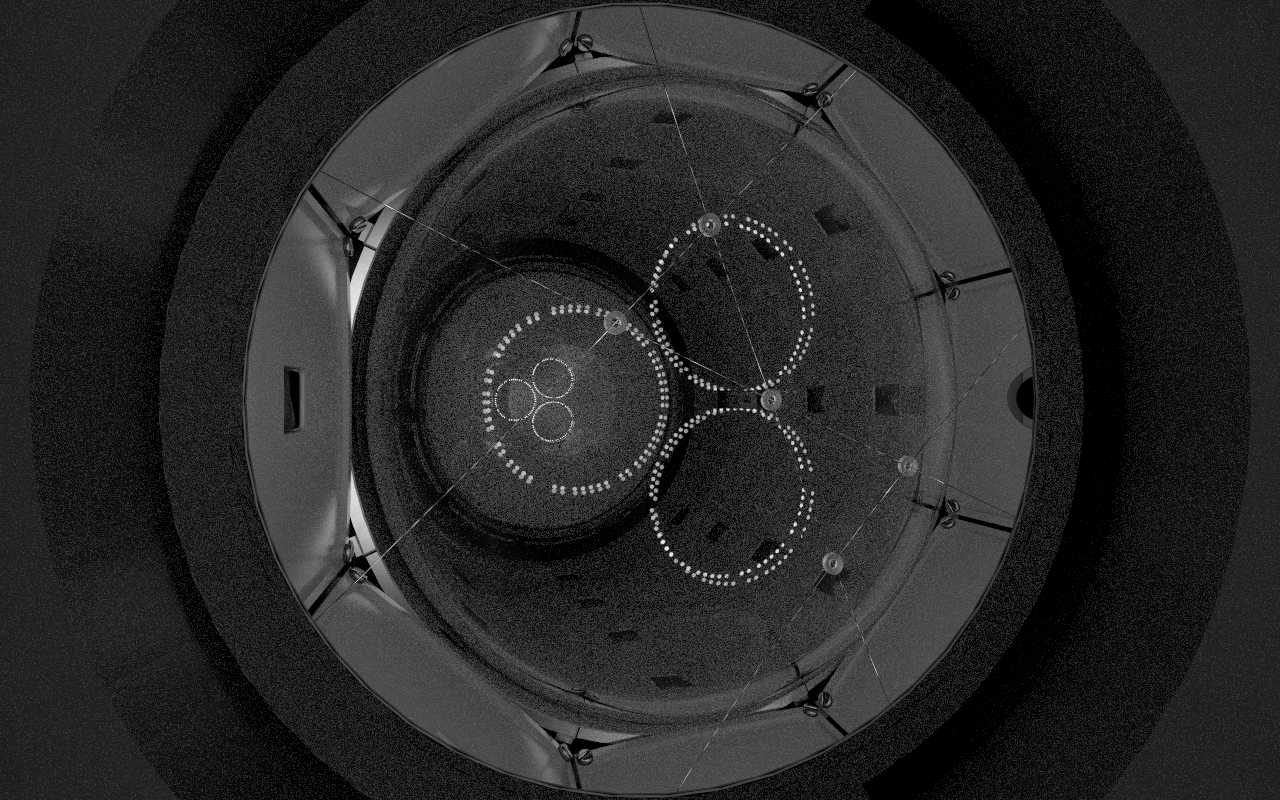
\includegraphics[width=0.33\textwidth]{render_with_fluid.png}}
    \caption{\textbf{(a)} A real image of the chamber with no fluids taken from camera 2 with a single LED ring turned on. \textbf{(b)} A rendered image of the chamber from camera 2 with ideal jar surfaces and all 3 LED rings turned on with no fluids in the chamber. \textbf{(c)} The same scene setup, now with fluids. Renders were taken with 4096 samples per pixel.}
    \label{fig:real_and_rendered_images}
\end{figure}

\subsection{Setting up the Scene to Render in Mitsuba} \label{subsec:setting_up_the_scene_to_render_in_mitsuba}
In order to render a scene in Mitsuba, we need to load in the scene either as a python dictionary or as an XML file -- in the code, we opted to use a python dictionary since we can adjust it dynamically. Each object in the scene is represented by an entry in the dictionary. For each object, we specify the file path to its triangle mesh\footnote{Mitsuba can only render triangle meshes and does not have support for $n$-gon meshes like Blender does.}, define the material either by manually entering the material properties or picking a pre-defined material within Mitsuba, and optionally set the object's transform. 

To compile the scene into a Mitsuba-readable dictionary, we first had to convert the existing CAD model into the individual components and set their materials. To do so, we began by exporting the CAD model of the inner vessel assembly of SBC-LAr10 (i.e., file X-A01-A) from SOLIDWORKS by saving the model as a polygon (`.ply') file.\footnote{When exporting the model from SOLIDWORKS, make sure to set the units for the model to centimeters!} This polygon file was then imported into Blender and the rotation of the model was adjusted so that the z-axis was parallel to the orientation of the jars. 

In Blender, the entire assembly was separated into its individual components. Then, any components that would not be visible to the cameras or indirectly visible in reflections were removed. The remaining components were grouped together primarily by material. For example, all of the metal screws became one group, the PTFE reflectors became another group, and the copper reflector supports became yet another group. Some other components were kept separated so that their positions could be individually manipulated such as the CF$_4$ feed line whose height was adjusted to match the relative position in the true images captured of the chamber. Notably, the LED rings had to be separated into their PCBs and each of the individual hemispherical emissive diodes were separated from the body of each LED in order to make sure the reflections of the LEDs on the jars remained circular. 

Parts of some components also had to be re-meshed because the exported polygon file had bad geometry for rendering. For example, the sides of the jars had to be re-created because the exported jars from the CAD models had long thin triangles which created rendering artefacts.\footnote{These rendering artefacts were caused by errors in the interpolated surface normals of the triangles. A common technique in order to create smooth meshes is to approximate the surface normals within the triangles in the mesh by interpolating between the defined normals at each triangle vertex. But if the vertices are too far apart, the approximation can cause artefacts.} In order to create smooth surfaces, large meshes such as the jars and reflectors were auto-smoothed such that for all vertices where neighboring vertex normals were within 30 degrees, the vertex normals were re-calculated to allow for smoother interpolation between individual triangle normals. In addition, parts of the viewports had holes in their model which needed to be filled in. The tops of the jar surfaces also needed to be re-meshed to create more vertices for applying distortion maps which are discussed later in this section.

Notably, all of the refractive surfaces had to be separated into their own individual components in order to properly assign the IoRs for each side of the surfaces. For example, the viewports were exported in groups of their outer surface and inner surface, and each of the jars were also separated into their outer and inner surfaces. See figure \ref{fig:chamber_materials} for more details on how these IoRs were assigned. In order to simulate a distorted jar surface, a radial ring texture map was created and applied as a displacement modifier along the vertex normals in Blender to the tops of each of the jars surfaces (see figure \ref{fig:distorted_jars_renders}). 

\begin{figure}[h]
    \centering
    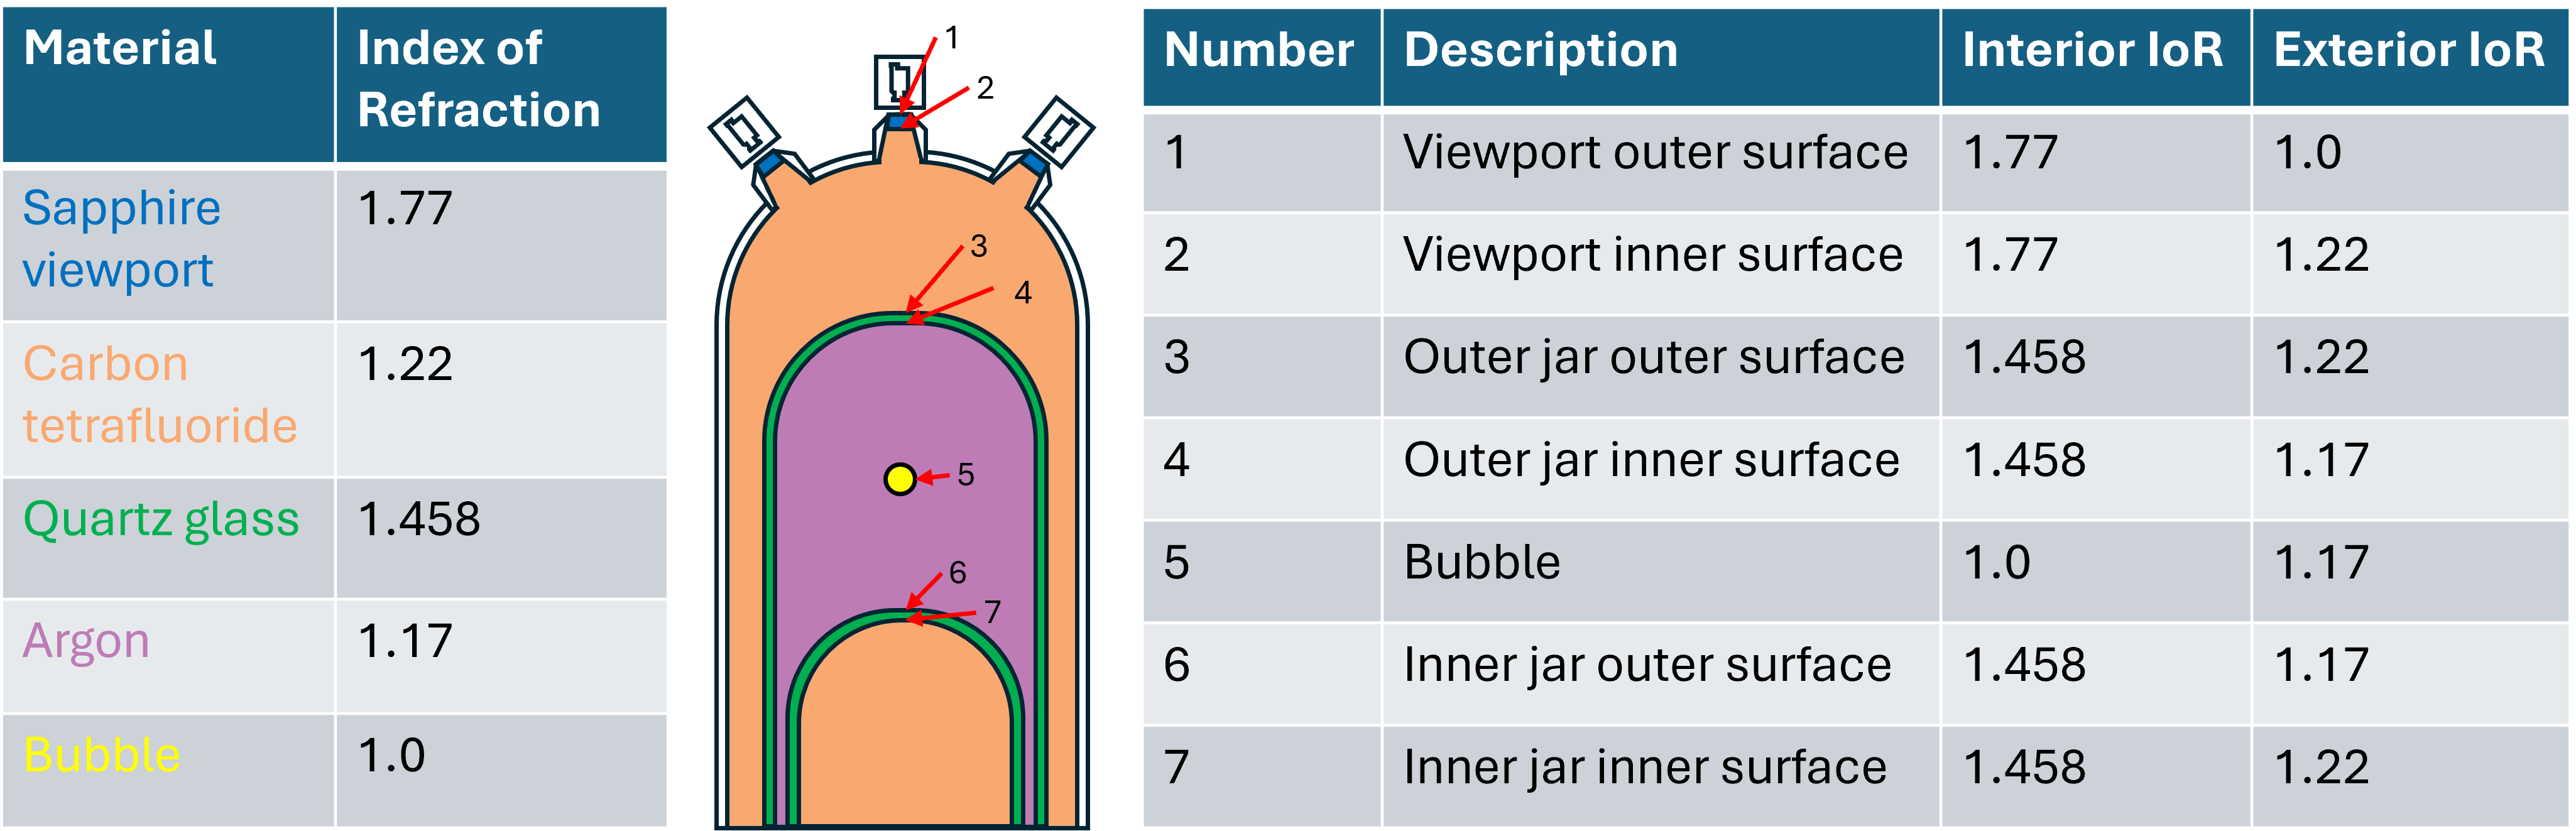
\includegraphics[width=0.9\textwidth]{chamber_materials.png}
    \caption{A diagram of refractive surfaces in the chamber. In order to accurately render the chamber, we need to individually define the interior and exterior IoRs for each surface. Note that the IoRs in the tables are estimates that were used in creating the renders but the true values may be different.}
    \label{fig:chamber_materials}
\end{figure}

\begin{figure}[h]
    \centering
    \subfloat{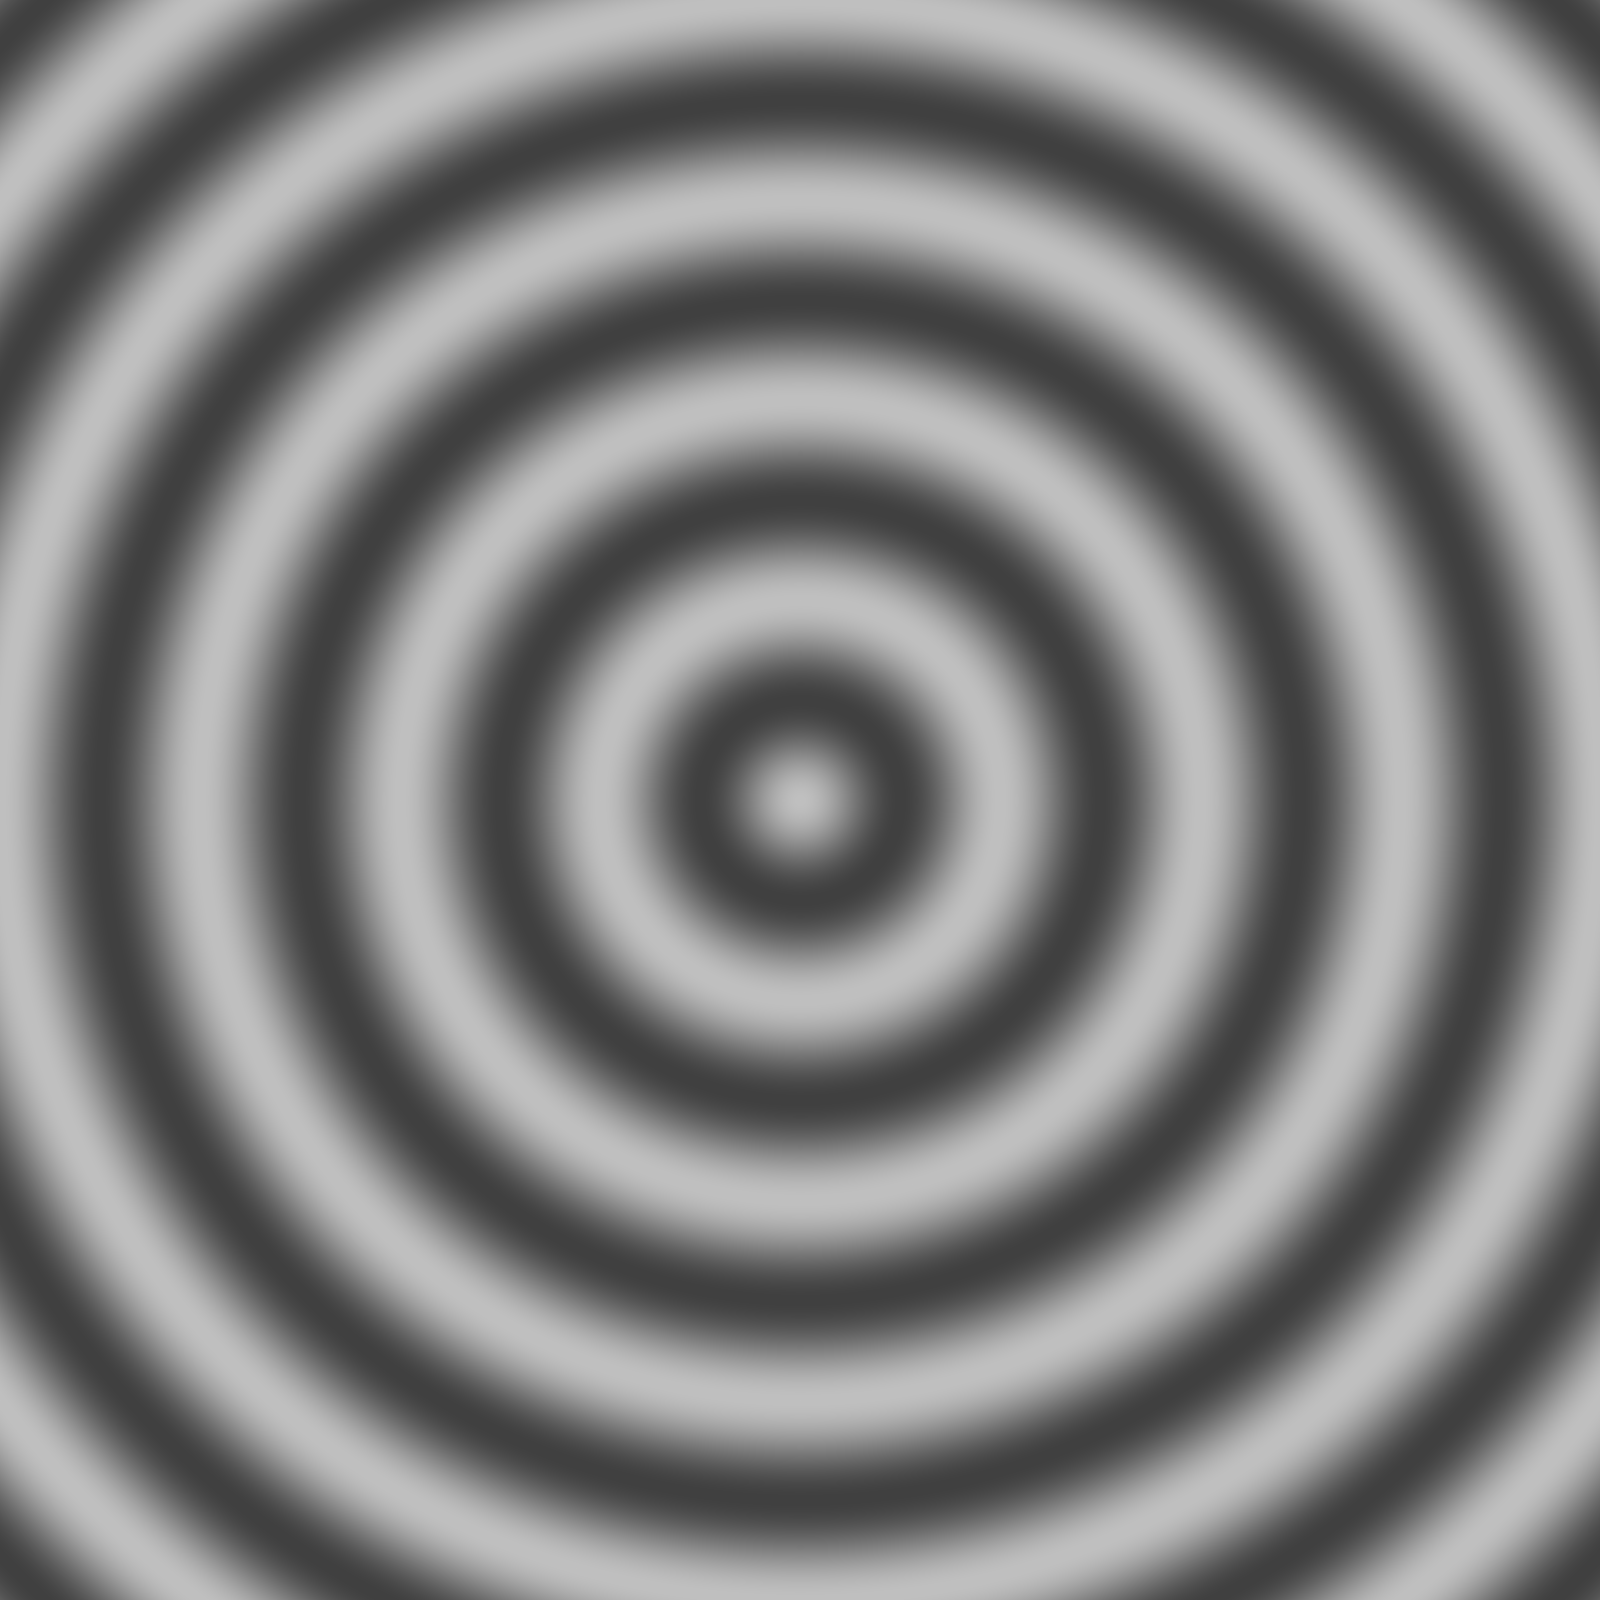
\includegraphics[height=1.5in]{rings.png}}
    \hfill
    \subfloat{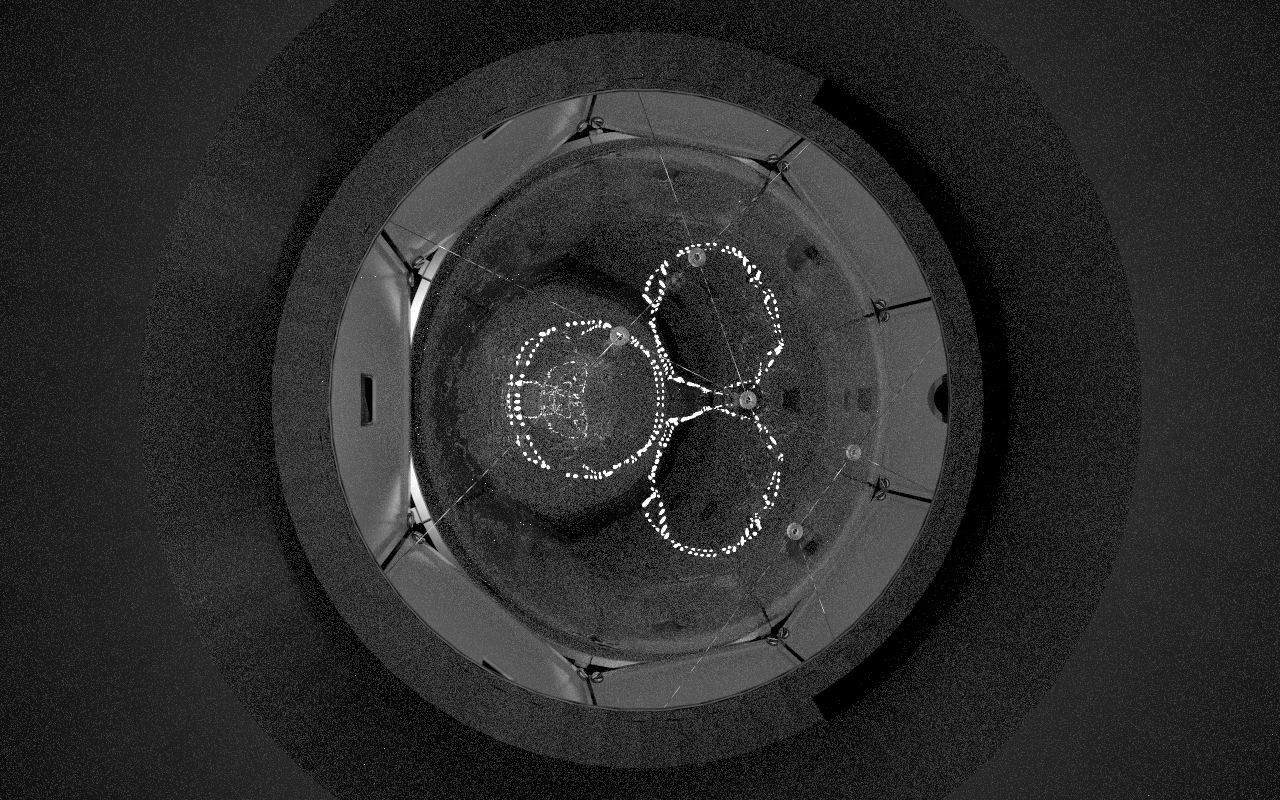
\includegraphics[height=1.5in]{distorted_jars_render_no_fluid.png}}
    \hfill
    \subfloat{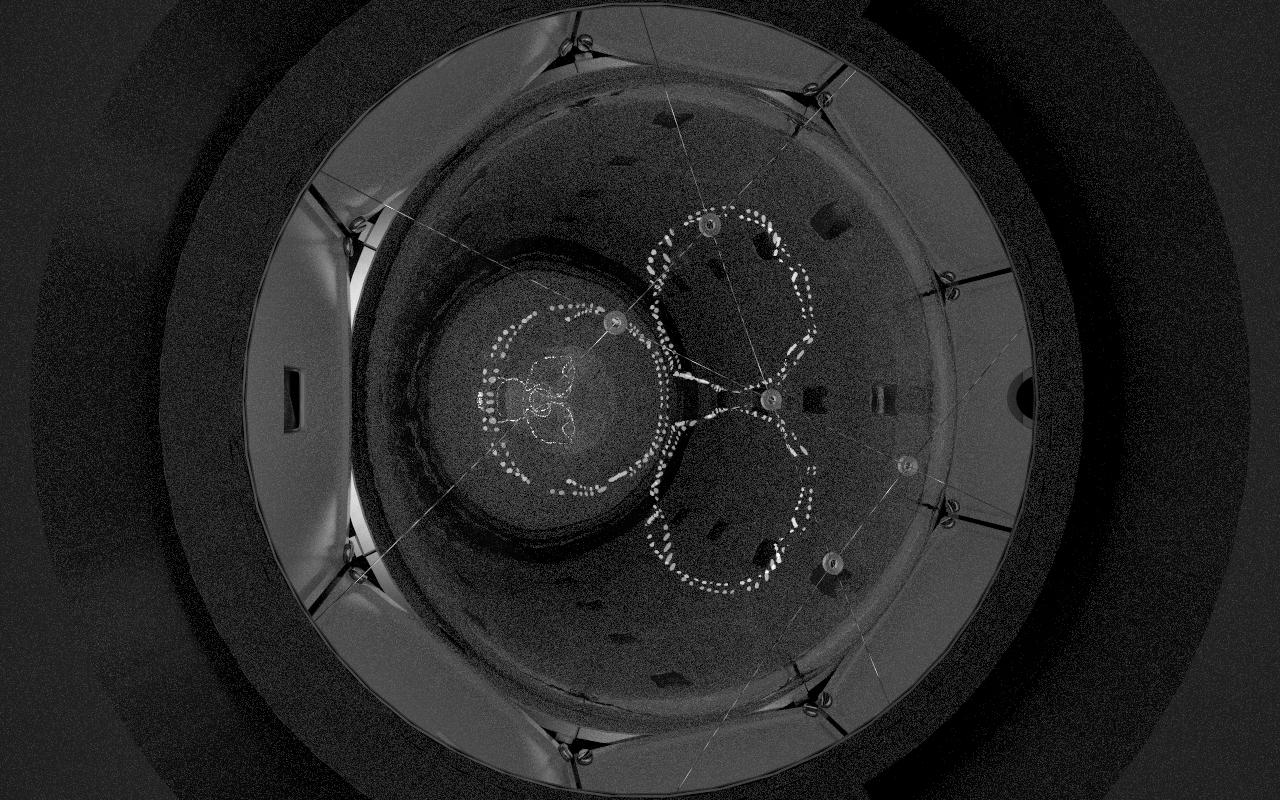
\includegraphics[height=1.5in]{distorted_jars_render_with_fluid.png}}
    \caption{\textit{(Left)} The radial ring distortion map used to displace the jar surfaces. \textit{(Center)} A rendered image of the chamber from camera 2 with the \textit{distorted} jar surfaces and all 3 LED rings turned on with no fluids in the chamber. \textit{(Right)} The same scene setup, now with fluids. Renders were again taken with 4096 samples per pixel. Compare these renders to figure \ref{fig:real_and_rendered_images}.}
    \label{fig:distorted_jars_renders}
\end{figure}

Once all components were adequately re-meshed and grouped, the whole assembly was moved so that the center fiducial marker of the chamber was located at the world origin and the jars were placed along $-z$. The model is also oriented so that the CF$_4$ feed line comes in from the $-x$ axis approximately ending at $x = 0$ cm. Once the relative position of all components was set (including any adjustments made to match the renders to existing images of the chamber), the origin for each group of components was set to be the world origin. This made it so that all vertices for the meshes within each group were now relative to the world origin so no transformations would need to be made when loading the models in to Mitsuba. Each component or group of components was then triangulated and exported as an individual mesh to be loaded into Mitsuba.

When each mesh was loaded into Mitsuba, their materials were assigned using the default Mitsuba materials wherever possible. The refractive surfaces were all modeled as dielectrics and their IoRs were set as in figure \ref{fig:chamber_materials}. The reflectivity of the PTFE and the brightness of the LEDs was manually adjusted to approximate the brightness and contrast of existing images of the chamber. Each LED ring was also loaded in as its own component so that each one could be turned `on' or `off' as desired for a given render. A `bubble' could be added to the scene by placing a dielectric sphere with a radius of a few millimeters somewhere within inter-jar volume with an exterior IoR equal to the LAr and the interior set to the IoR of a vacuum. 

The camera positions for the renders were calculated by first determining the center positions of the outer viewport surfaces and their corresponding surface normals in Blender. The cameras were then positioned at the viewport centers plus 1 cm along the outer viewport surface normals and were oriented along the negative of the surface normal. This is in contrast to the true chamber where the positioning of the cameras is not as exact and would need to be estimated using the fiducial markers (see \S\ref{subsec:the_pose_matrix}). 

\subsection{Testing Setup} \label{subsec:testing_setup}
In order to test and benchmark the algorithms in this paper, renders of a grid of points were created with and without the refractive surfaces (including the jar surfaces and viewports). This allowed for the comparison of 2D pixel and 3D world localizations with and without the refractive surfaces in the chamber, all while the corresponding true positions of those 3D points and their 2D image projections was known. 

The outer jar in the model has an inner radius of 11.5 cm and a thickness of 0.5 cm such that the outer surface of the jar has a radius of 12 cm. The top of the outer jar's curved top surface is approximately \textit{within} 1 cm below the central fiducial marker with the curved top surface extending to approximately 6 cm below it. The distance to the lower jar's top surface is approximately 23 cm from the fiducial markers in the model, though in practice this height can change to increase or decrease the pressure in the inter-jar volume. Therefore, the chosen grid for testing was a cylindrical grid with 5 evenly spaced layers extending from $z=-6$ cm down to $z=-18$ cm where each layer consisted of a central point plus 8 concentric rings of evenly spaced points with the outer-most ring extending out to a radius of 11 cm. Each layer consisted of 200 points, so in total there were 1000 points in the grid approximately evenly distributed throughout the working volume of the target fluid (see figure \ref{fig:testing_grid}).

\begin{figure}[h]
    \centering
    \subfloat[3D projection]{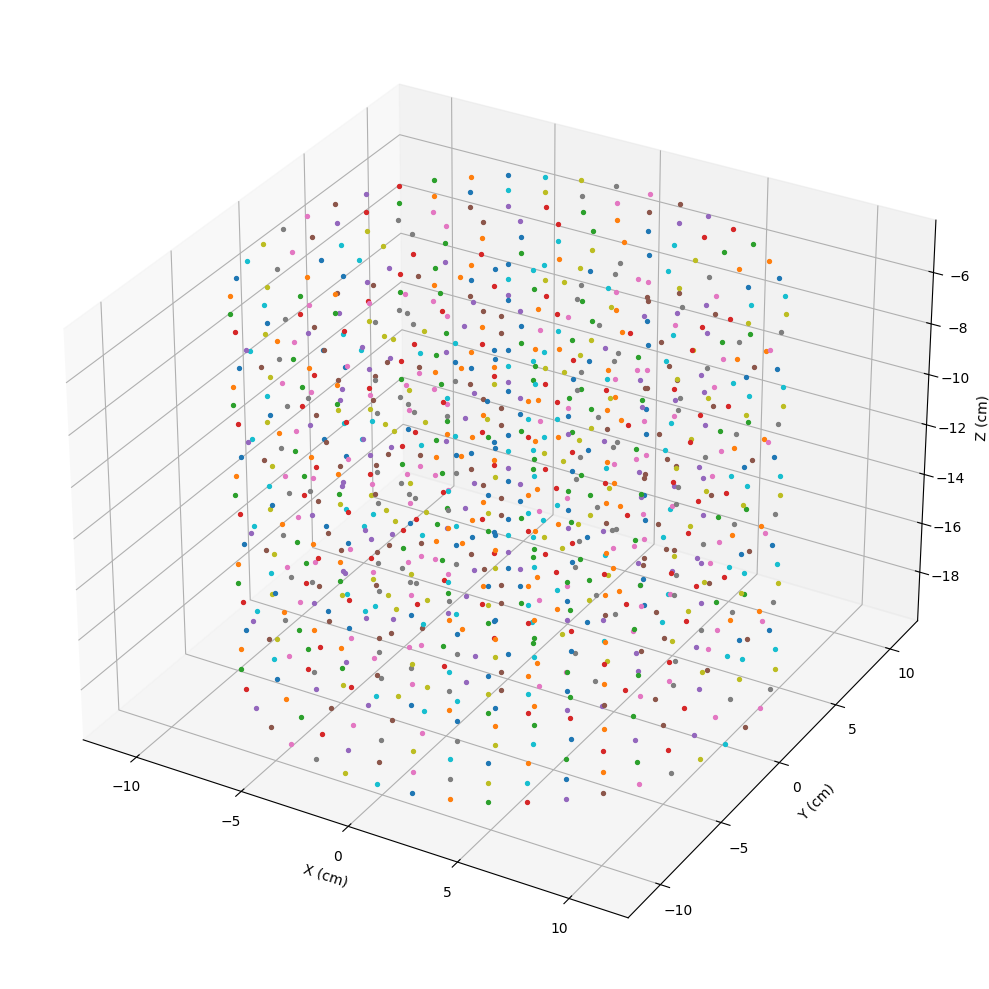
\includegraphics[height=2.8in]{testing_grid_3d.png}}
    \hfill
    \subfloat[Single-layer 2D projection]{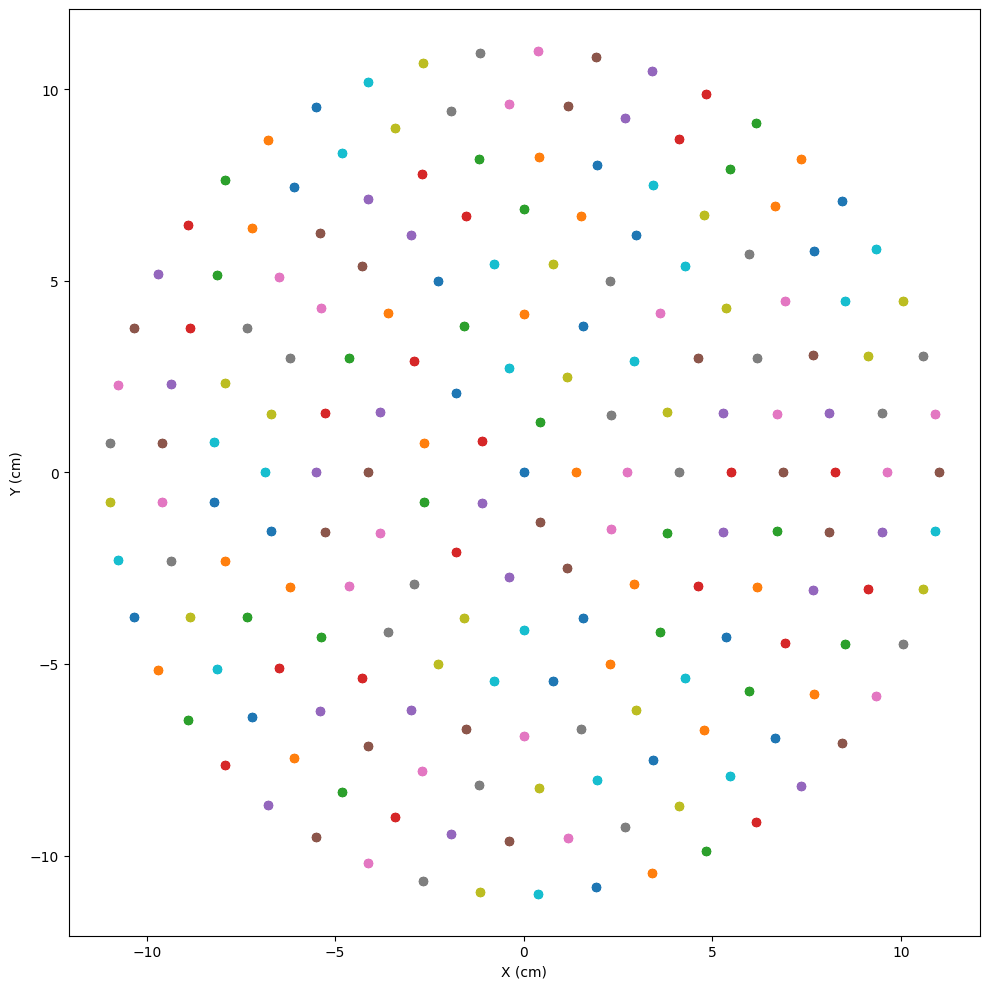
\includegraphics[height=2.8in]{testing_grid_2d.png}}
    \caption{The grid used to test and benchmark the algorithms in this paper consisted of 1000 points approximately evenly distributed throughout the inter-jar volume in a cylindrical pattern.}
    \label{fig:testing_grid}
\end{figure}

For each grid point, a render of the chamber was created with and without the refractive surfaces where the point in the image was represented by a spherical light source (see figure \ref{fig:grid_lights}). Setting the point as a light source instead of an actual `bubble' made it easier to determine the location of the point within the image using the circle Hough transform as in \S\ref{subsec:circle_hough_transform}, since the focus of these tests was on triangulation and remapping and not detection. In addition to determining the locations of the points using the Hough transform, the exact grid positions of each point were also known and their exact 2D image projections could be computed by multiplying the world position of the point with the pose and camera matrices as in equation \ref{eq:camera_intrinsic_extrinsic}. 

\begin{figure}[h]
    \centering
    \subfloat[]{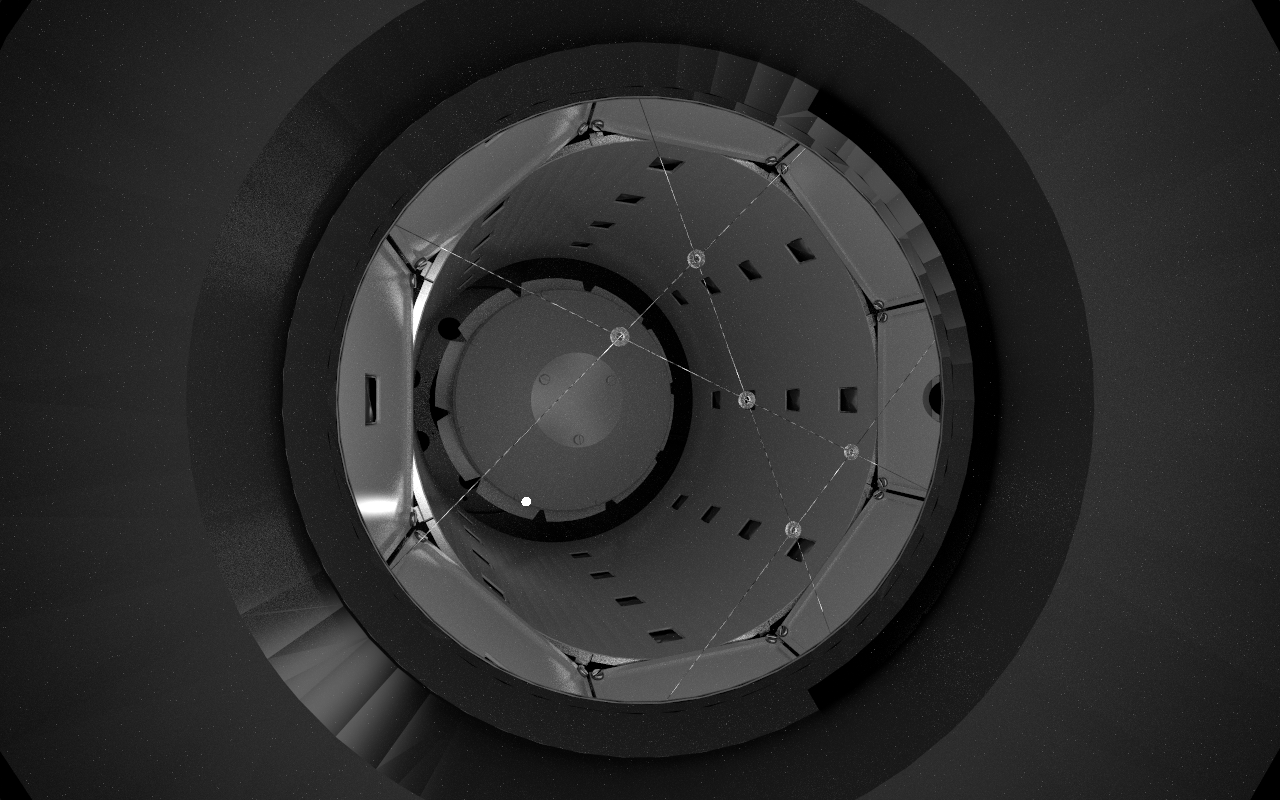
\includegraphics[width=0.33\textwidth]{light_no_refract.png}}
    \hfill
    \subfloat[]{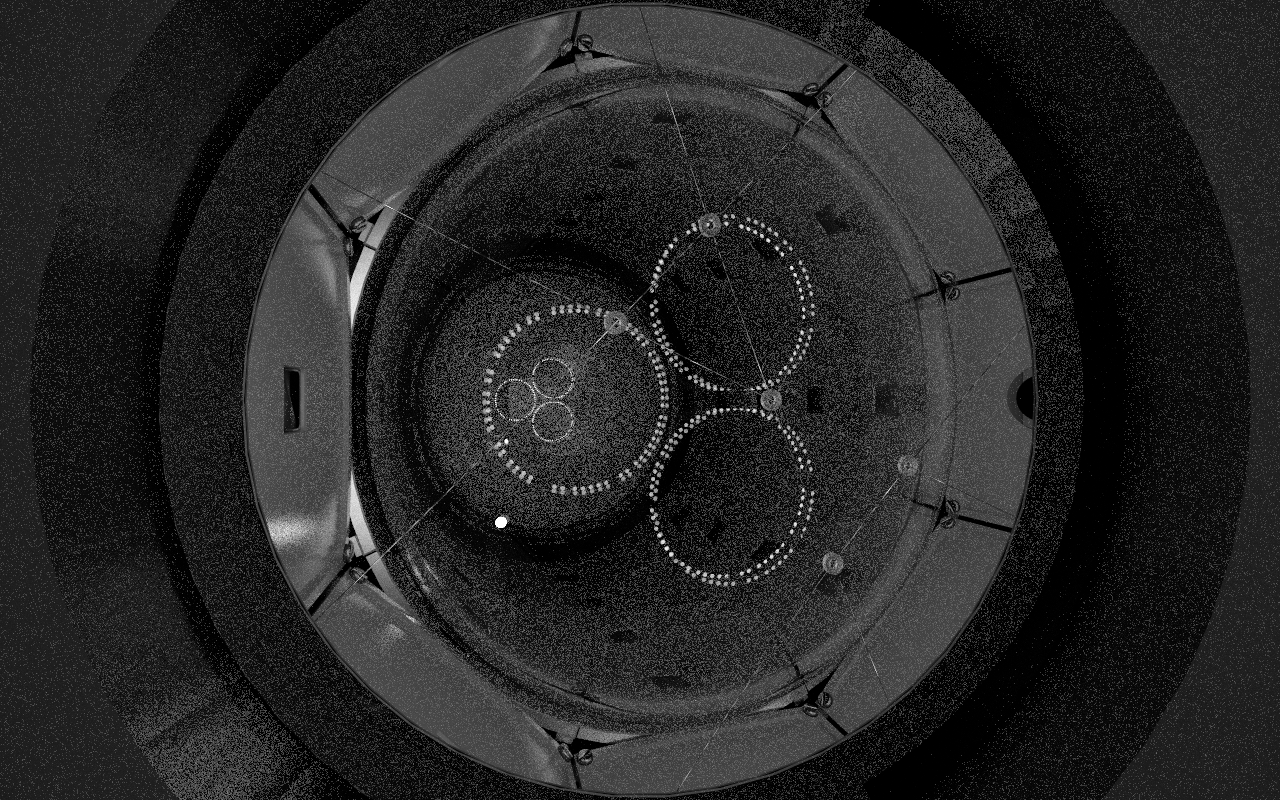
\includegraphics[width=0.33\textwidth]{light_ideal.png}}
    \hfill
    \subfloat[]{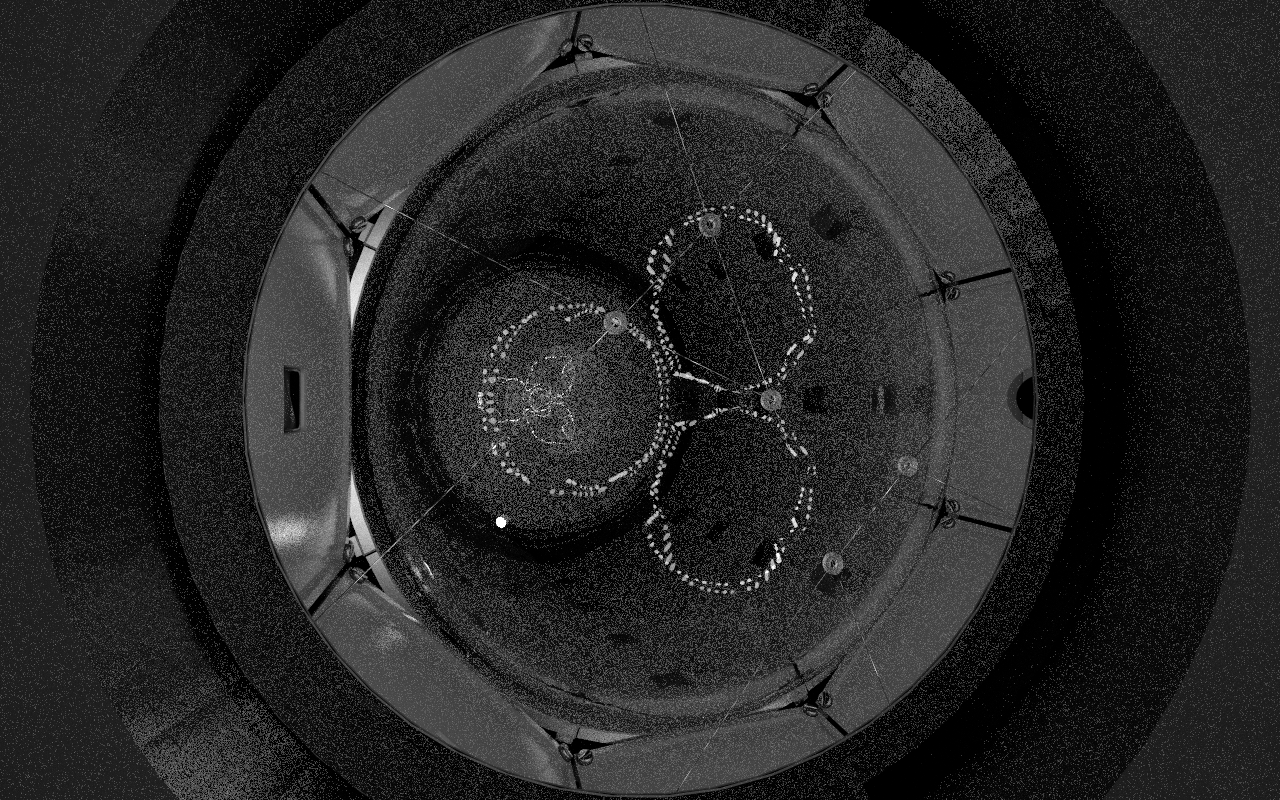
\includegraphics[width=0.33\textwidth]{light_distorted.png}}
    \caption{Testing of the algorithms was done by creating a render of each point in the grid from figure \ref{fig:testing_grid} without \textbf{(a)} and with refractive surfaces using either ideal jar surfaces \textbf{(b)} or distorted jar surfaces \textbf{(c)} as well as using the true grid positions and their image projections. The grid points were rendered as light sources to make localization in the images easier. These images were rendered with 1052 samples per pixel but the true testing images only used 16 samples per pixel since all we needed was to detect the circle of light in the image which converges much faster.}
    \label{fig:grid_lights}
\end{figure}

\subsection{Path Tracing}\label{subsec:path_tracing}
To create the renders as seen in figures \ref{fig:real_and_rendered_images} and \ref{fig:distorted_jars_renders}, the \textit{path tracer} integrator built into Mitsuba was used. Path tracing is a type of ray tracing algorithm. While many types of ray tracing algorithms exist, fundamentally they are all trying to solve the \textit{rendering equation}, also sometimes referred to as the \textit{light transport equation (LTE)} \cite{pharr2023physically}\footnote{See \S13.1 of \cite{pharr2023physically} for a deeper explanation of the LTE. Note that they use slightly different variable names than are used here. The expression of the LTE in equation \ref{eq:lte} uses more standard notation compared to \cite{pharr2023physically}.}:
\begin{align}\label{eq:lte}
    L_o(\mathbf{x}, \omega_o) = L_e(\mathbf{x}, \omega_o) + \int_\Omega f_r(\mathbf{x}, \omega_i, \omega_o) L_i(\mathbf{x}, \omega_i) (\omega_i \cdot \mathbf{n}) \mathrm{d} \omega_i
\end{align}
where
\begin{itemize}
    \item $\mathbf{x}$ is a position in space.
    \item $\omega_o$ is the direction of the outgoing ray.
    \item $\omega_i$ is the direction of the incident ray.
    \item $\mathbf{n}$ is the surface normal at $\mathbf{x}$.
    \item $\Omega$ represents that the integral is over the unit hemisphere around $\mathbf{n}$ such that $\omega_i \cdot \mathbf{n} > 0$.
    \item $L_o$ is the outgoing radiance from position $\mathbf{x}$ in the direction $\omega_o$.
    \item $L_e$ is the emitted radiance from position $\mathbf{x}$ in the direction $\omega_o$.
    \item $L_i$ is the incoming radiance at position $\mathbf{x}$ from direction $\omega_i$.
    \item $f_r$ is the bidirectional scattering distribution function.
\end{itemize}
Except for the most basic scenes, the LTE is not analytically solvable so ray tracing algorithms try to approximate it numerically using a Monte Carlo approach\footnote{A Monte Carlo integration algorithm refers to any type of algorithm which tries to approximate the integral by some form of random sampling.}. The most basic ray tracing algorithm, for example, simply shoots rays from the sensor into the scene and lets them bounce around the scene until they either hit a light source or hit their bounce limit. This method will eventually converge but it is expensive and slow, especially for scenes where the probability of a ray hitting a light source is small. 

Path tracing improves upon the basic ray tracing algorithm by trying to find a complete path along which light can travel from an emitter to the sensor for each bounce of the ray \cite{jakob2022mitsuba3} (see figure \ref{fig:path_tracer}). An important piece of this algorithm is the bidirectional scattering distribution function (BSDF) ($f_r$ in equation \ref{eq:lte}). In basic ray tracing, the BSDF is used to generate an outgoing ray direction at each surface interaction depending on the incoming ray direction at a point on a surface (see figure \ref{fig:bsdf_overview}). Different types of surfaces will have different BSDFs. For example, the BSDF for a mirror-like surface will be a delta function in the direction which is a reflection of the incoming ray direction. Meanwhile, the BSDF for a perfectly diffuse surface will be the uniform hemisphere around the surface normal. For path tracing, the BSDFs are also used for \textit{importance sampling}.

\begin{figure}[h]
    \centering
    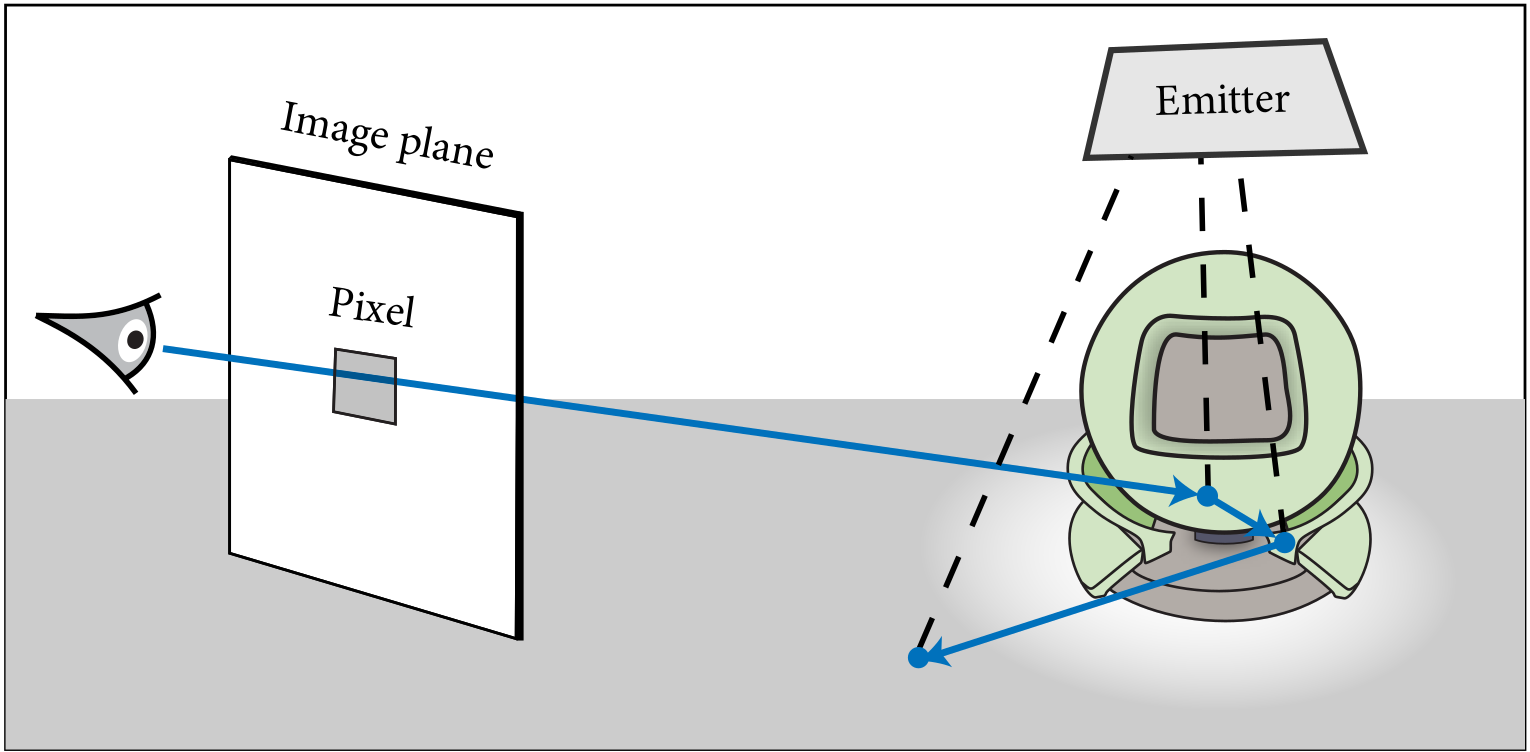
\includegraphics[width=0.75\linewidth]{figures/integrator_path_figure.png}
    \caption{The path tracer integrator in Mitsuba operates by performing random walks for the ray path just as the basic ray tracing algorithm would. However, it also utilizes importance sampling by trying to create direct connections to the emitters in the scene at each surface intersection. Figure courtesy of \cite{jakob2022mitsuba3}.}
    \label{fig:path_tracer}
\end{figure}

\begin{figure}[h]
    \centering
    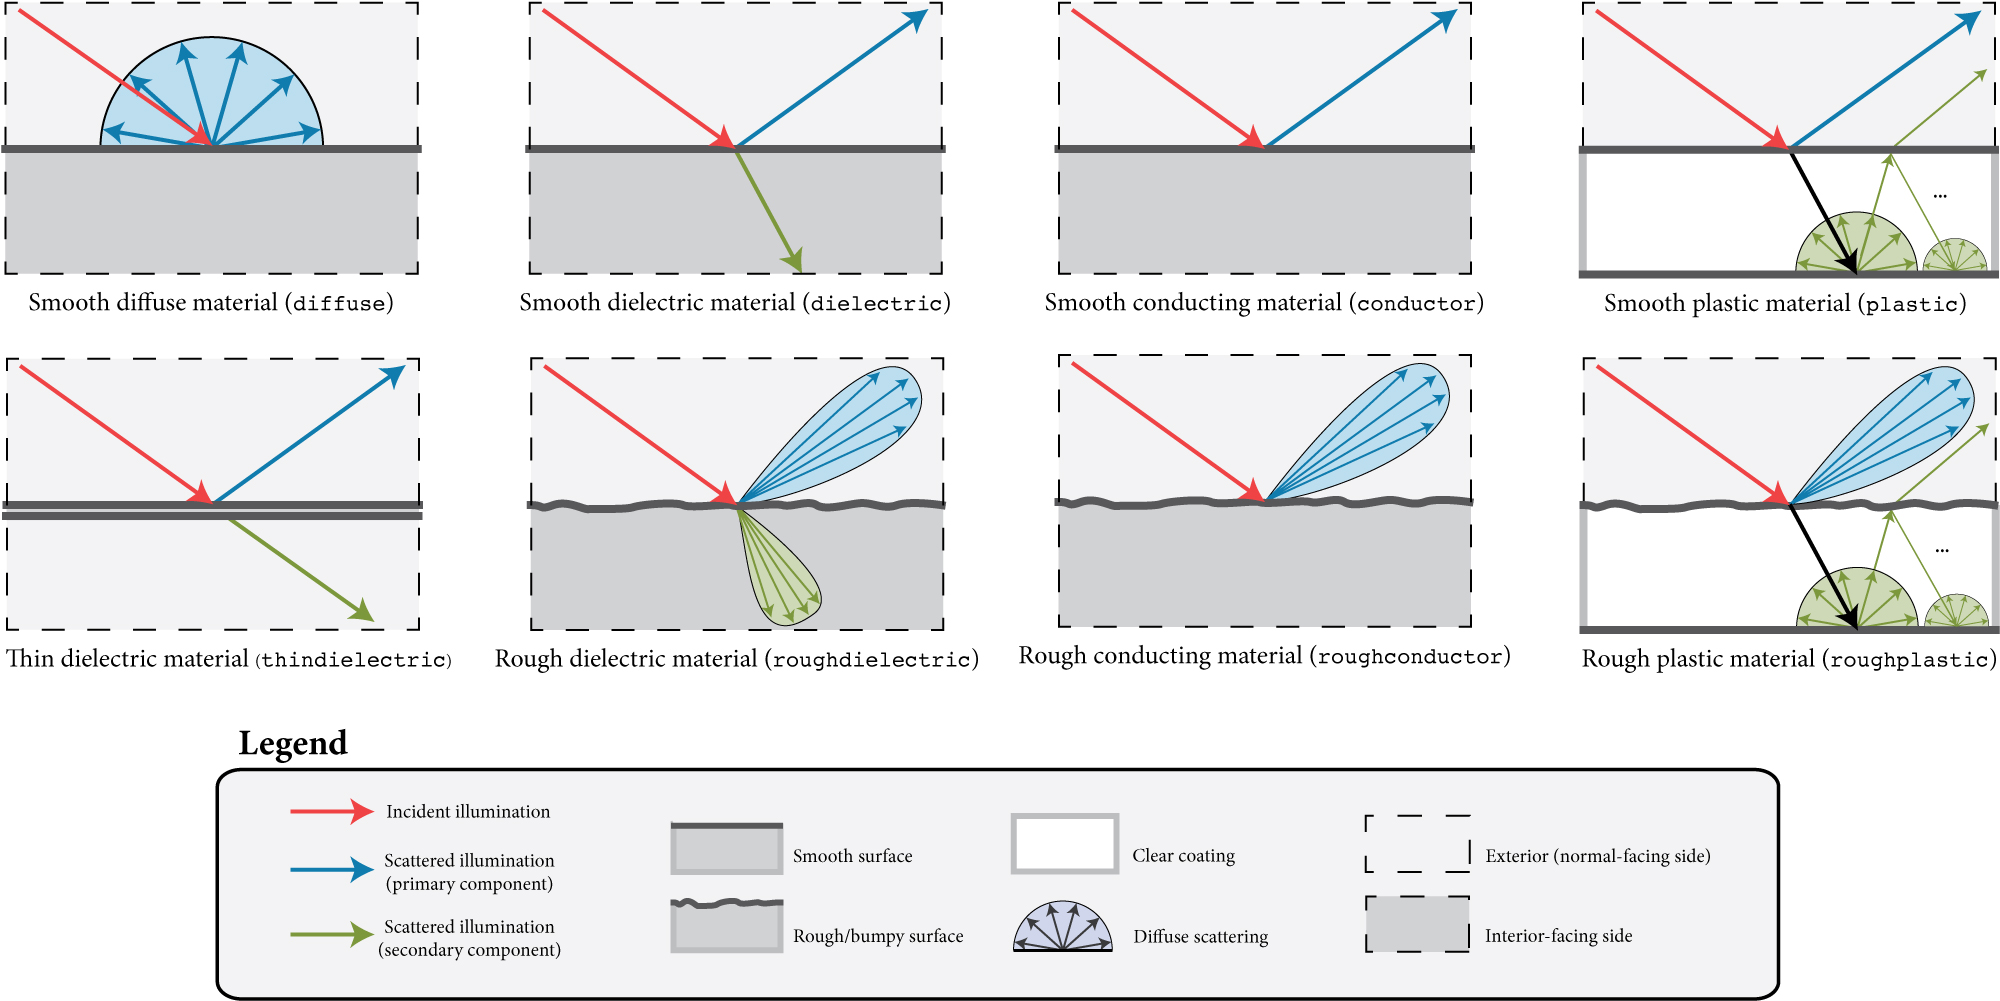
\includegraphics[width=\linewidth]{figures/bsdf_overview.jpg}
    \caption{A schematic of the different types of bidirectional scattering distribution functions available in Mitsuba 3. Figure courtesy of \cite{jakob2022mitsuba3}.}
    \label{fig:bsdf_overview}
\end{figure}

As described earlier, path tracing tries to determine a direct connection to a light source at each bounce of the ray. By doing so, they do not need to rely on a given ray randomly hitting a light source to start illuminating the surfaces in a scene. Instead, at each bounce of the ray, the contribution of a given light source that is directly visible at that surface intersection point is scaled by the BSDF for outgoing rays in the direction of that light source. The scale factor for the light contribution is determined by integrating the projection of the visible portion of the emitter from that intersection point onto the unit hemisphere around the surface normal multiplied by the BSDF for that surface interaction. Effectively, this is a more direct computation of the integral in equation \ref{eq:lte} compared to what would be done with basic ray tracing which would require many more rays for the same result.

Note that the importance sampling strategy for path tracing only works when there are no occluders between a given point of intersection and a light source. This means that path tracers work best in scenes where the emitters are ``easily accessible'' by the objects in the scene. Consider our scene of the chamber. The only objects in the scene that are directly illuminated by the LEDs are the top reflectors, the fiducial markers, and the outer-most surface of the outer jar (see figure \ref{fig:direct_illumination_components}). The rest of the scene, i.e., everything within the glass jars, does not have a direct connection to the LEDs since the jars technically act as occluders. This means that renders of our scene with the jars will be more noisy given the same sample count since they cannot make use of the importance sampling which is particularly unfortunate for our use case. Despite this, the path tracer integrator is still the best available integrator in Mitsuba for creating renders of our scene. Though, there may be alternate renderers which feature integration methods better suited to scenes with occluding transparent surfaces.

\begin{figure}[h]
    \centering
    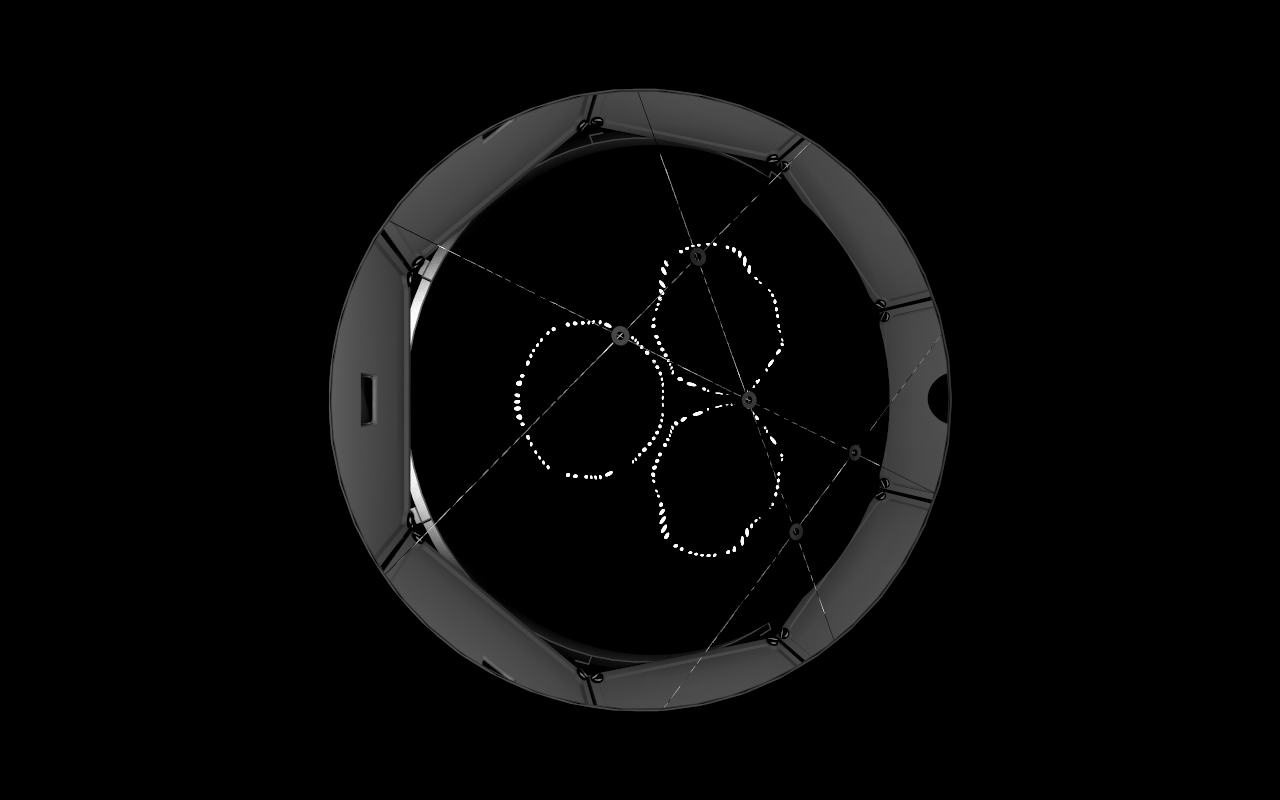
\includegraphics[width=0.5\linewidth]{direct_illumination.png}
    \caption{Portions of the chamber that are directly illuminated by the LEDs. Note how only the primary reflections off the top jar are visible. This image can be rendered by setting the bounce limit to 4 (2 bounces to get through the viewports, 1 bounce to hit the surfaces, 1 bounce to reach a light source).}
    \label{fig:direct_illumination_components}
\end{figure}


\section{Bubble Detection} \label{sec:bubble_detection}
This section discusses a potential method for determining the initial pixel location of a bubble within an image as well as its apparent radial size in pixels known as the \textit{circle Hough transform} (\S\ref{subsec:circle_hough_transform}). Later in \S\ref{subsec:corresponding_bubbles}, we also discuss how we can determine which bubbles correspond with one another between images if more than one bubble is present in each image.

\subsection{Circle Hough Transform} \label{subsec:circle_hough_transform}
The \textit{circle Hough transform} is an algorithm for detecting circles within an image with some pre-defined radius. Like other Hough transform algorithms, it relies on creating an accumulator for possible circles within the image. However, compared to other Hough transforms such as the transform for a line, the accumulator space will always have the same aspect ratio as the image, and no pixel transformations are necessary except for potentially a uniform scale factor. To start, we pass in an edge map of the original image using an algorithm such as the \textit{Canny edge detector}. Then, for each pixel in the edge map, we draw a corresponding circle of the given radius we are searching for in the accumulator space. If a circle with the matching radius exists in the image, the accumulator space will have a corresponding peak at the (potentially scaled) pixel location of the center of the bubble in the original image (see figure \ref{fig:circle_hough_transform_accumulator_a}). Then, to determine if an arbitrary size circle exists within the image, we need to repeat the process for all circle radii we want to search for. This effectively creates a 3D accumulator space where a cone is created from each position in the edge map and the 3D position where the accumulator surpasses a given threshold represents a detected circle's pixel position and radius (see figure \ref{fig:circle_hough_transform_accumulator_b}).

\begin{figure}[h]
    \centering
    \subfloat[\label{fig:circle_hough_transform_accumulator_a}]{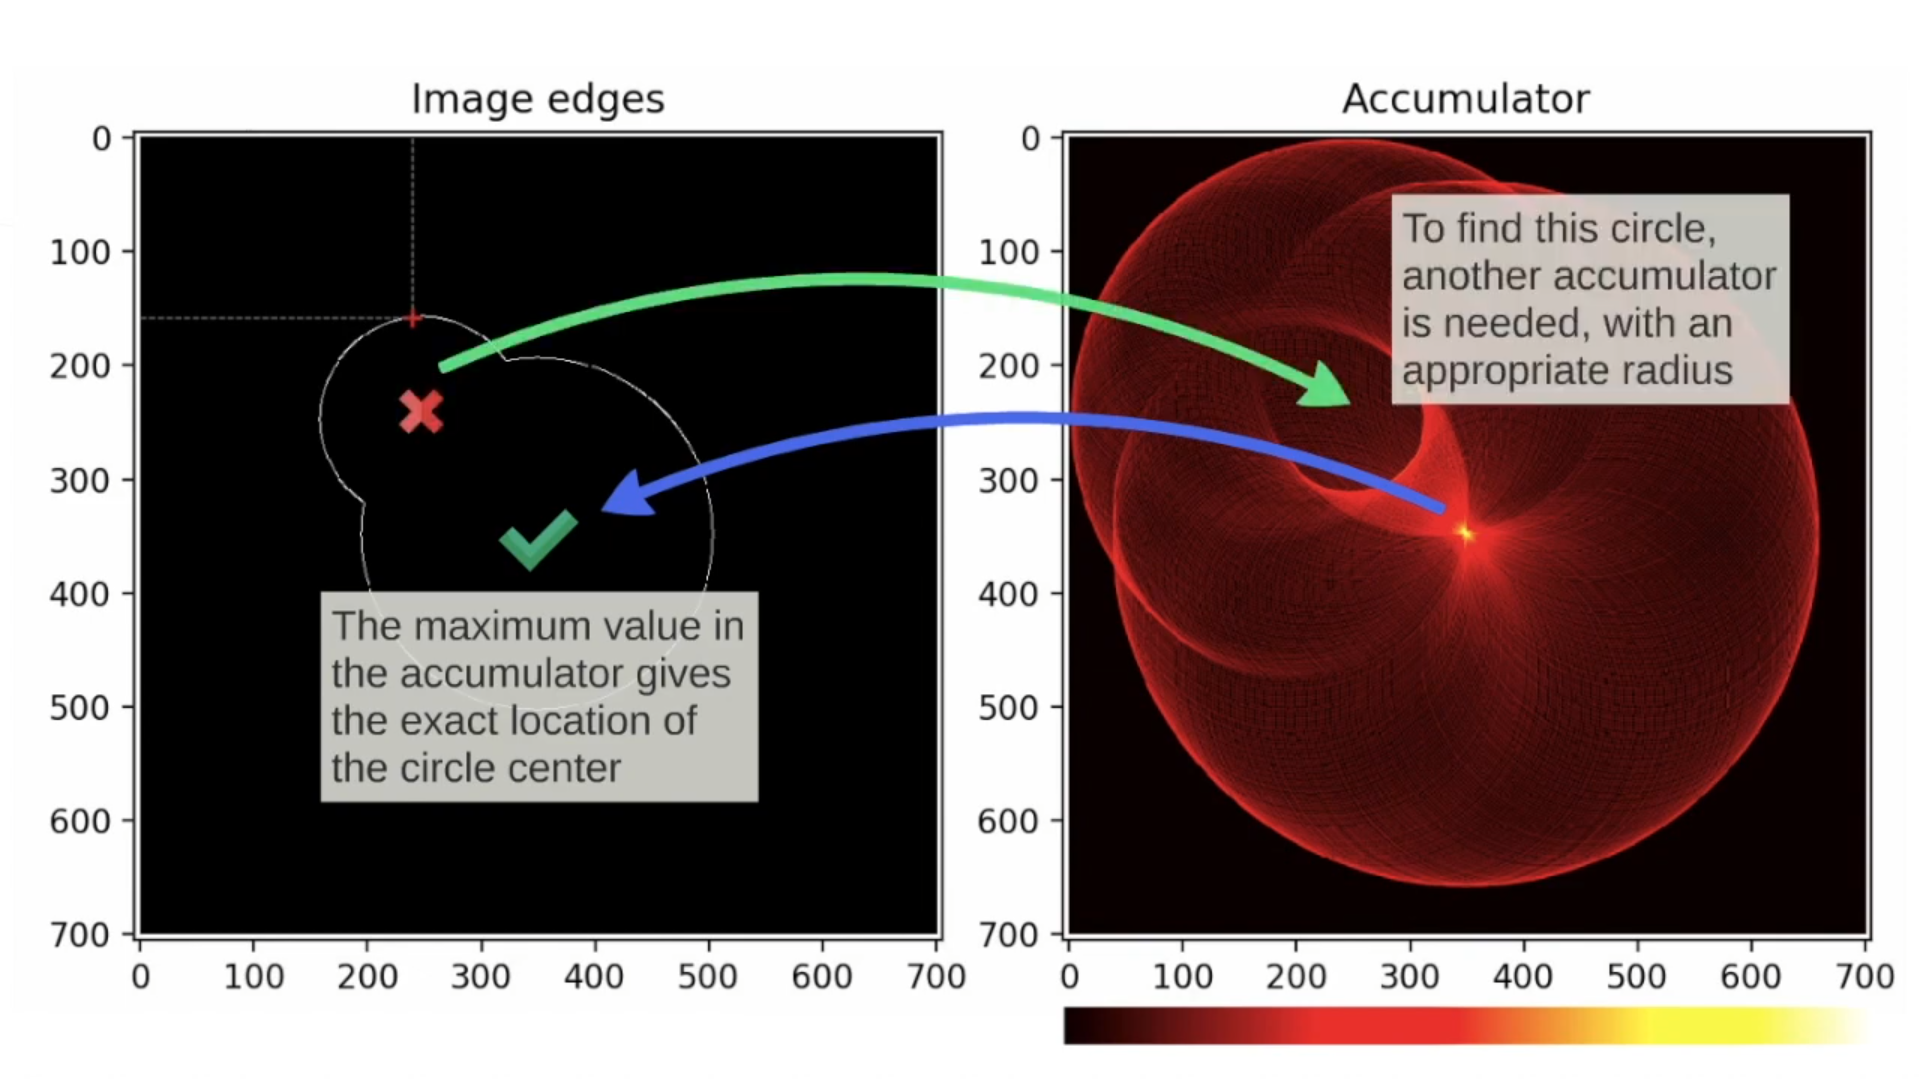
\includegraphics[height=2in]{hough_transform_accumulator.png}}
    \hfill
    \subfloat[\label{fig:circle_hough_transform_accumulator_b}]{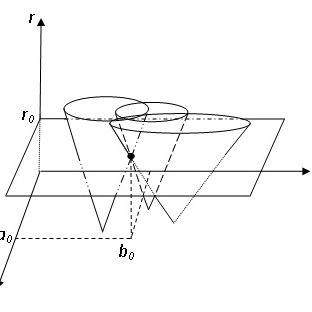
\includegraphics[height=2in]{hough_transform_accumulator_cones.jpg}}
    \caption{\textbf{(a)} On the left is an edge map of an image with two apparent circles within it. On the right, we create a 2D accumulator space for the Hough transform, drawing a circle centered at each pixel of the edge map with a radius equal to the target circle we are searching for. In the accumulator space, the maxima corresponds to the location of the circle center with that radius. Figure courtesy of Thales Sehn Körting. \textbf{(b)} A 3D accumulator space searching for circles with a range of radii. A cone emanates from each pixel position in the edge map. Points where multiple cones intersect such that the accumulator passes a certain threshold indicates potentially detected circles with a given center and radius. Figure courtesy of \cite{djekoune2017incremental}.}
\end{figure}

In practice, we can improve the detection of circles and remove extraneous circle detection (e.g., the circles formed in the images by the viewports, the jars themselves, the reflections of the LED rings, etc.) by doing \textit{background subtraction}. Since our cameras are stationary and we have access to images from before and after bubble nucleation, we can isolate the pixels in the image which have changed since a bubble was created. To do so, we simply subtract the image in which a bubble appears from the background image with no bubble. Then, if we normalize the range of the resulting image between 0 to 1 (or between 0 to 255 as integers), the brightest pixels in the difference image will be where the bubbles are located. \footnote{Note that we subtract the target image from the background image instead of vice versa because the bubbles appear in the images as dark rings, so the normalized difference image will appear as black with bright regions where the bubbles are instead of bright with dark regions for the bubbles. This does not affect the performance of the Hough transform since the image gets passed through the Canny edge detector first which is not impacted by this choice.} We can also speed up the detection of circles by reducing the size of the image input to the Hough transform by cropping the image to only the region which contains the jars. However, this hasn't been implemented since the performance boost is minor, especially for an offline application, and would require a little bit of extra book keeping to make sure pixel positions are represented correctly in the cropped images.

In the code, we are using OpenCV's built-in `HoughCircles' method to locate the bubbles for testing with the `HOUGH\_GRADIENT\_ALT' flag (see the documentation of \cite{opencv_library}). One limitation of this method is its inability to determine the \textit{sub-pixel} location of the bubble center. At best, it provides positions in half-pixel increments. Therefore, one method to potentially provide better sub-pixel accuracy is to use the background subtracted image to compute the \textit{center of mass} of the region where the circle was detected. More specifically, we can compute edge map of the background subtracted image with the canny edge detector (using OpenCV's `Canny' method), return the original values of the corresponding pixels of the edge map, crop to the region where the circle was detected, and find the center of mass of that cropped region. This should provide better sub-pixel accuracy for the bubble position in the images, though this has not been implemented or tested yet. For a discussion of the impact that sub-pixel accuracy has on localization, see \S\ref{sec:summary_of_error_contributions} and figure \ref{fig:pixel_remapping_error_on_triangulation_accuracy}.

\subsection{Corresponding Bubbles} \label{subsec:corresponding_bubbles}
One way to determine which bubbles correspond to each other between each camera view is to make use of epipolar constraints. A single pixel position from one view corresponds to a ray of real-world positions. That ray, for another camera with no distortion, corresponds to a line (called an \textit{epipolar} line) of possible positions in the other view (see figure \ref{fig:epipolar_geometry}). Therefore, one way to determine corresponding object positions between the views is to find the object in the second view that is closest to the projected epipolar line of the point in the first view. Note that in order for this method to work, we would need to use the undistorted positions of the bubbles determined using the methods described in \S\ref{subsec:magnification_from_refractive_surfaces} and \S\ref{subsec:jar_surface_distortions}.

% Unfortunately, this method works best when the images have no distortion. If lenses were the only source of distortion, then the images could be undistorted and the epipolar line would remain straight. However, because our images feature distortion within the scene itself, a single point in one image can correspond to multiple ray segments as the outgoing ray from the sensor refracts through the jars. We could get around this issue by using the undistorted points from both cameras that are remapped using the methods described in \S\ref{subsec:magnification_from_refractive_surfaces} and \S\ref{subsec:jar_surface_distortions}.

\begin{figure}[h]
    \centering
    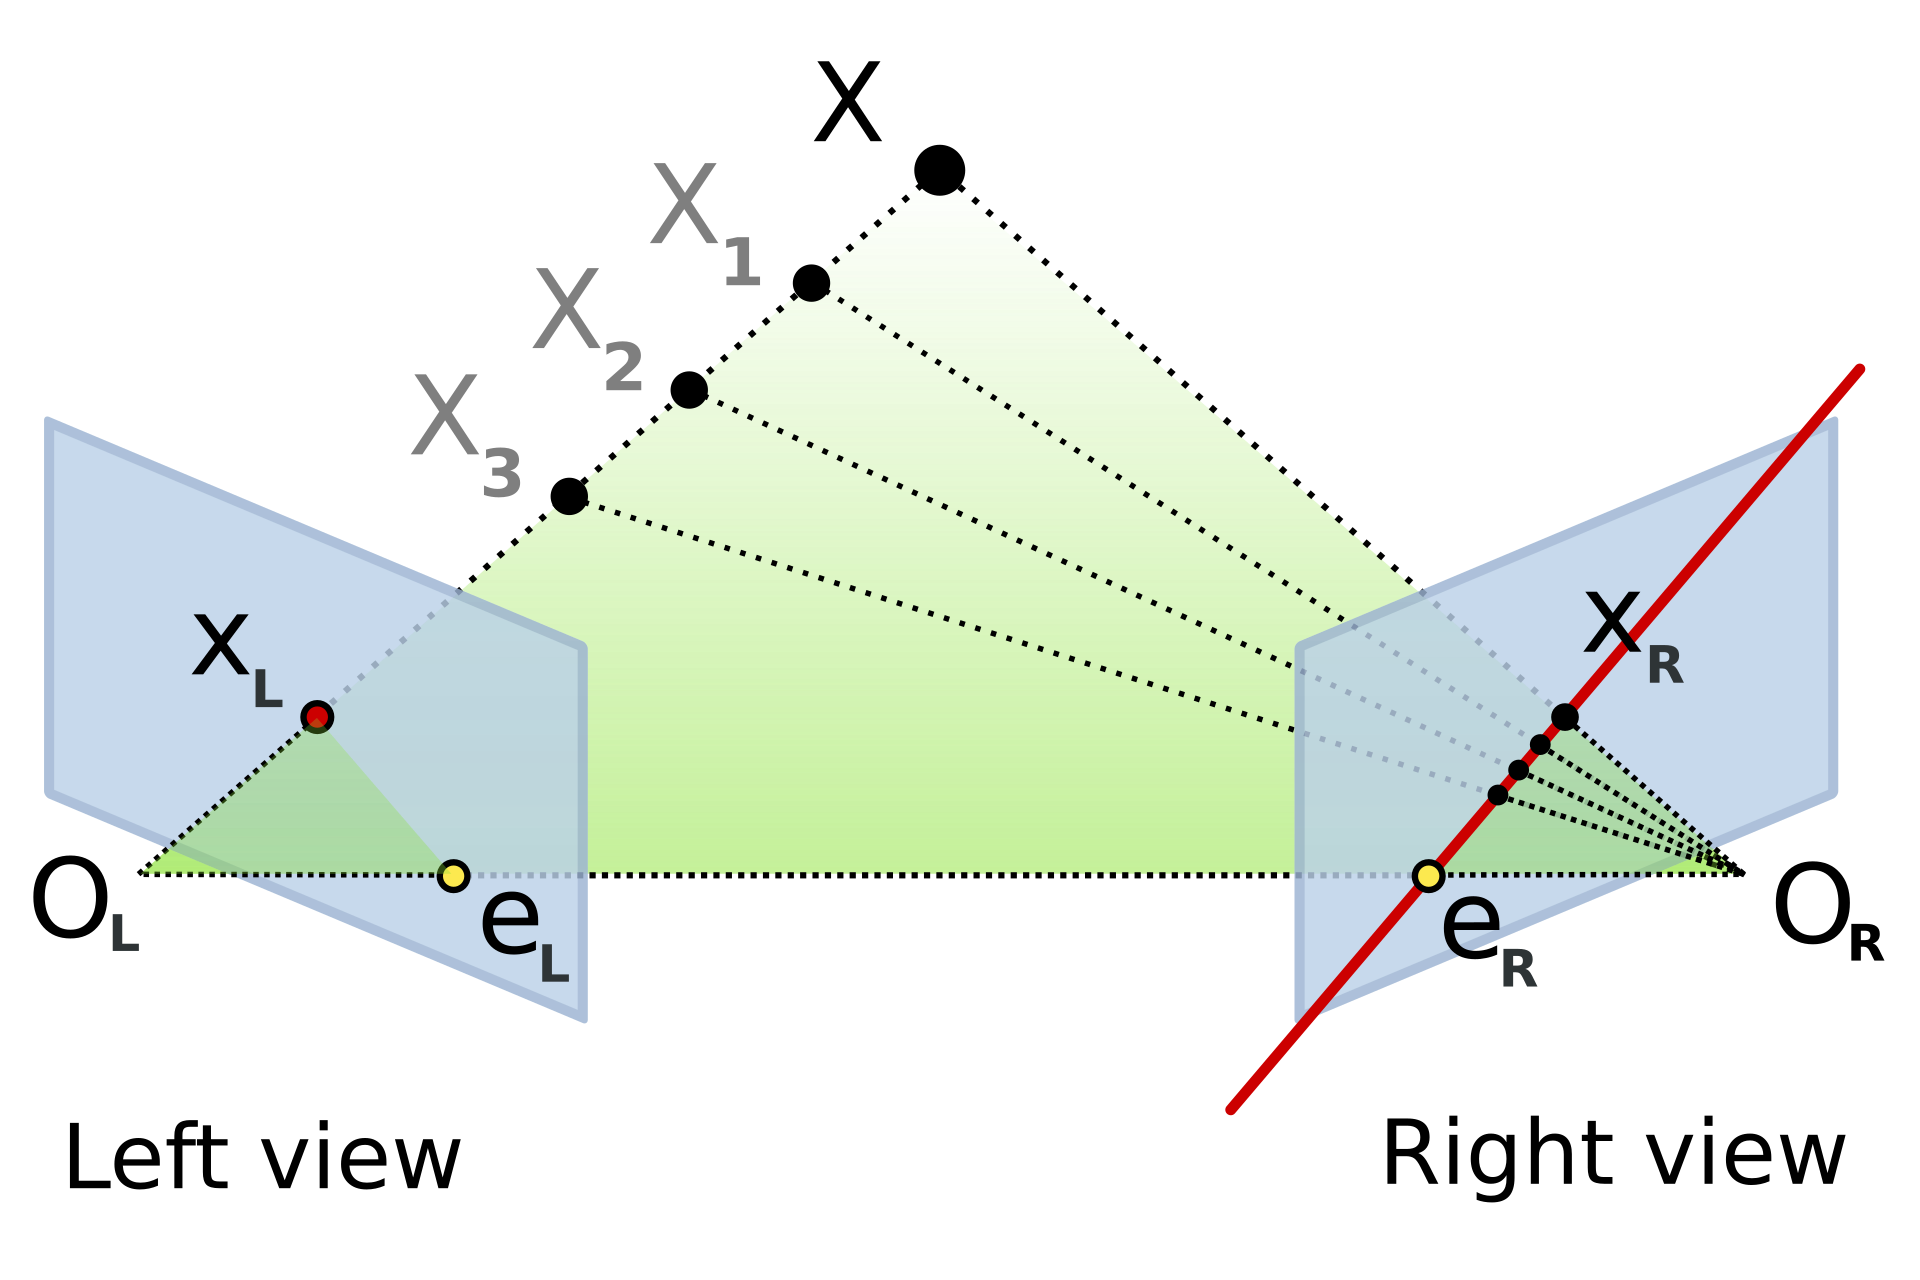
\includegraphics[width=0.5\linewidth]{epipolar_geometry.png}
    \caption{A pixel position $X_L$ from the left view corresponds to a line of possible positions $\overline{e_R X_R}$ in the right view due to epipolar geometry. Therefore, one way to determine corresponding bubbles between the cameras is to find the bubble positions from the second and third cameras that are closest to the corresponding epipolar line $\overline{e_R X_R}$. However, this method works best when there are no distortions present in the image. Figure courtesy of Arne Nordmann.}
    \label{fig:epipolar_geometry}
\end{figure}

However, a more straightforward approach is to use a slightly modified version of the mid-point two view triangulation method described later in \S\ref{subsec:mid-point_two_view_triangulation}. If we modify equation \ref{eq:midpoint_two_view_H} to instead return the \textit{distance} between the points of closest intersection of the rays, we can simply do a brute-force search for the corresponding bubble positions in each view whose undistorted outgoing rays have the closest points of intersection. I.e., equation \ref{eq:midpoint_two_view_H} can be modified to solve for the distance between $d_{ij}$ between ray $r_i$ from view one and $s_j$ from view two:
\begin{align}
    d_{ij} = || \overline{F_i G_j} || = || G_j - F_i || = || Q_j + \mu_j \bar{s_j} - P_i - \lambda_i \bar{r_i} ||.
\end{align}
This method has been tested and shown to provide accurate bubble correspondences as long as the pixel localizations of the bubbles in the images are sufficiently far apart compared to the average error in the pixel localizations.

\section{Dealing With Distortions} \label{sec:dealing_with_distortions}
In order to triangulate a bubble's position, we need to shoot rays as close as possible to the true bubble position starting from the camera origins and then determine the point of closest intersection of the corresponding rays from all of the cameras. Unfortunately, the refractive surfaces between the bubble and each of the camera sensors distort the pixel position that the bubble gets projected to. Rays fired in the direction of the distorted projections will entirely miss the true bubble position. Therefore, we need to account for the distortions in the images to remap the projected pixel position of the bubble as if there were no distortion-inducing refractive elements. In the following subsections, we will first evaluate the relationship between pixel localization error and triangulation error to determine the scale of error propagation. Then, we will cover the different sources of distortion and discuss models that can be utilized to undistort the bubble projections. 

An important note for the following subsections is that determining the coefficients used in the models relies on creating renders of the chamber. With the renders, we can simulate the bubble projections with and without the distortive elements or even directly project the bubbles onto the sensors since the their true positions and exact projection matrices of the cameras are known. Using the distorted and undistorted positions is what allows us to solve for the coefficients of a distortion function using a linear least-squares approach. However, that does not necessarily mean that these models are useless in practice where the true bubble positions are unknown. If the model of the chamber is accurate to the true chamber, the distortion remapping functions computed with the renders will be applicable to the true images as well. However, this does require that the model of the chamber is \textit{very close} to the true chamber as even minor deviation in the refractive indices of the elements can cause significant increases in the localization error. See \S\ref{subsec:impacts_of_remapping_errors_on_triangulation_accuracy} and figure \ref{fig:pixel_remapping_error_on_triangulation_accuracy} for a discussion on how remapping errors propagate to localization errors.

\subsection{Impacts of Remapping Errors on Triangulation Accuracy} \label{subsec:impacts_of_remapping_errors_on_triangulation_accuracy}
In order to determine the relationship between errors in pixel localization and errors in triangulation, the ground truth pixel positions of all 1000 grid points from figure \ref{fig:testing_grid} were first determined by projecting them onto the camera sensors using the ideal camera matrices and known pose matrices from the renders as in equation \ref{eq:camera_intrinsic_extrinsic}. Then, a random pixel offset within some pre-defined radius was applied to each of the localizations from each camera view and the distorted points were then used to triangulate the points using N-view triangulation. This was repeated for a number of maximum radii for pixel offsets, taking the average triangulation error over several runs with each maximum offset. The resulting graph (figure \ref{fig:pixel_remapping_error_on_triangulation_accuracy}) shows a strong linear relationship between the average expected triangulation error and the average pixel localization error.\footnote{The x-axis was converted from the maximum offset to the average offset by scaling the x-axis by $2/3$ since the average distance from the center for a point in the unit circle is $2/3$.} Note that this graph assumes all pixel localizations are offset by some random amount in any direction so it does not effectively account for systematic errors (e.g., say if all pixel positions are uniformly shifted in some direction), but it should provide clues regarding aggregate errors.

\begin{figure}
    \centering
    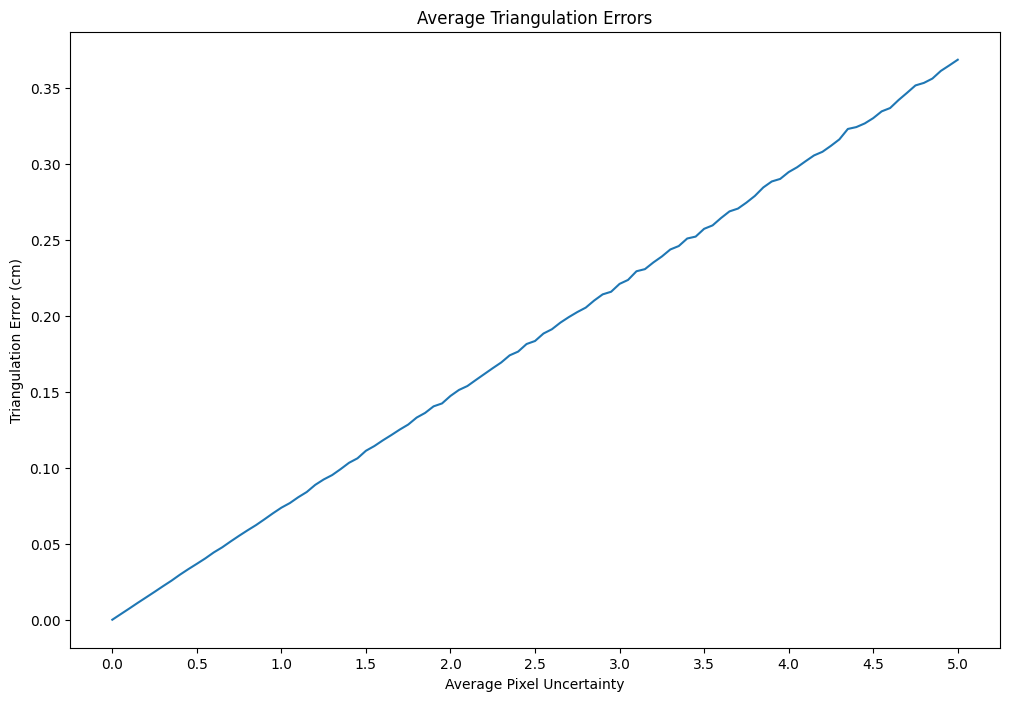
\includegraphics[height=3in]{average_triangulation_error_based_on_pixel_localization_error.png}
    \caption{A graph of average triangulation error as a function of average pixel localization error. The graph shows a linear relationship between improving pixel remapping accuracy and triangulation error. The best fit line for this graph is $y = 0.073606x - 1.43555\times 10^{-5}$. Therefore, for sub-millimeter accuracy, our average pixel localization error needs to be within 1.36 pixels assuming we have a perfect match for camera pose.}
    \label{fig:pixel_remapping_error_on_triangulation_accuracy}
\end{figure}

\subsection{Camera Calibration} \label{subsec:camera_calibration}
Camera lenses used to focus an image to the camera sensor can introduce a significant amount of distortion to the images. Often, this distortion is radial, causing parallel lines in an image to bend or warp (see figure \ref{fig:radial_distortion_examples} for different types of radial distortion). In addition, if the lens' focus plane is not parallel to the sensor, then the resulting image can also be skewed, known as \textit{tangential distortion}. 

\begin{figure}[h]
    \centering
    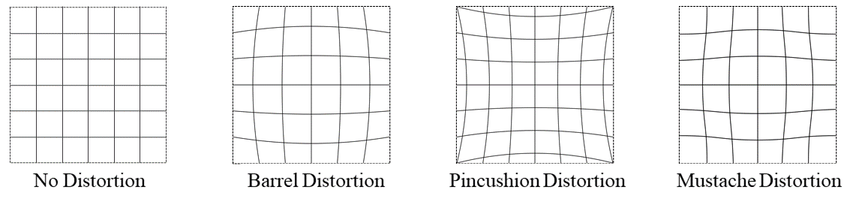
\includegraphics[width=0.9\linewidth]{radial_distortion_examples.png}
    \caption{Examples of different types of radial distortion that can be caused by camera lenses. The wide angle, fish eye lenses used in the chambers seem to produce \textit{mustache distortion}, characterised by having opposing signs for the coefficients $k_1$ and $k_2$ in equations \ref{eq:camera_radial_distortion_model_x} and \ref{eq:camera_radial_distortion_model_y}. See \S\ref{subsubsec:zhang's_method_for_camera_calibration} for previously computed distortion coefficients. Figure courtesy of \cite{fan2020computer}.}
    \label{fig:radial_distortion_examples}
\end{figure}

In this subsection, we will introduce the general model for camera distortions and briefly discuss how the distortion coefficients can be solved as a least-squares problem. Then, we will briefly discuss how these distortion coefficients are often calculated in practice using \textit{Zhang's method} as first introduced in \cite{zhang2000flexible}. Finally, we will discuss the existing work on determining the radial distortion of the camera lenses used in SBC-LAr10 performed by Ethan Rengifo.

\subsubsection{The General Camera Distortion Model} \label{subsubsec:the_general_camera_distortion_model}
Let $x = x_0 - x_c$ and $y = y_0 - y_c$ where $x_0, y_0$ are the original distorted pixel coordinates and $x_c, y_c$ are the pixel coordinates of the center of the image (i.e., we move the origin of the pixel coordinates to the centers of the images). Also, let $r^2 = x^2 + y^2$ and let $x', y'$ be the undistorted pixel coordinates. The general model for distortions caused by camera lenses can then be represented as:
\begin{align} 
    \label{eq:camera_radial_distortion_model_x} x' &= x + x(k_1 r^2 + k_2 r^4 + k_3 r^6) + p_1(r^2 + 2x^2) + 2p_2 xy \\ 
    \label{eq:camera_radial_distortion_model_y} y' &= y + y(k_1 r^2 + k_2 r^4 + k_3 r^6) + 2p_1 xy + p_2 (r^2 + 2y^2).
\end{align}
Here, $k_1, k_2, k_3$ are the radial distortion coefficients and $p_1, p_2$ are the tangential distortion coefficients. We can factor these into matrix multiplication form. For x:
\begin{align}
    \nonumber x' &= x + x(k_1 r^2 + k_2 r^4 + k_3 r^6) + p_1(r^2 + 2x^2) + 2p_2 xy \\
    \nonumber    &= x + x k_1 r^2 + x k_2 r^4 + x k_3 r^6 + x p_1 \left(\frac{r^2}{x} + 2x \right) + x p_2 (2y)\\
    \nonumber \frac{x'}{x} - 1 &= k_1 r^2 + k_2 r^4 + k_3 r^6 + p_1 \left(\frac{r^2}{x} + 2x \right) + p_2 2y\\
    \frac{x'}{x} - 1 &= 
    \begin{bmatrix}
        r^2 & r^4 & r^6 & \left(\frac{r^2}{x} + 2x \right) & 2y
    \end{bmatrix}
    \begin{bmatrix}
        k_1 \\ k_2 \\ k_3 \\ p_1 \\ p_2
    \end{bmatrix},
\end{align}
and for y:
\begin{align}
    \nonumber y' &= y + y(k_1 r^2 + k_2 r^4 + k_3 r^6) + 2 p_1 xy + p_2 (r^2 + 2y^2) \\
    \nonumber    &= y + y k_1 r^2 + y k_2 r^4 + y k_3 r^6 + y p_1 (2x) + y p_2 \left(\frac{r^2}{y} + 2y \right)\\
    \nonumber \frac{y'}{y} - 1 &= k_1 r^2 + k_2 r^4 + k_3 r^6 + p_1 2x + p_2 \left(\frac{r^2}{y} + 2y \right)\\
    \frac{y'}{y} - 1 &=
    \begin{bmatrix}
        r^2 & r^4 & r^6 & 2x & \left(\frac{r^2}{y} + 2y \right)
    \end{bmatrix}
    \begin{bmatrix}
        k_1 \\ k_2 \\ k_3 \\ p_1 \\ p_2
    \end{bmatrix}.
\end{align}
Then, we can set these up into the form $A \mathbf{x} = b$ for $n$ pairs of distorted and undistorted points and try to solve for $\mathbf{x}$:
\begin{align}
    \nonumber A \mathbf{x} &= b \\
    \begin{bmatrix}
        r_1^2 & r_1^4 & r_1^6 & \left( \frac{r_1^2}{x_1} + 2x_1 \right) & 2y_1 \\
        r_1^2 & r_1^4 & r_1^6 & 2x_1 & \left( \frac{r_1^2}{y_1} + 2y_1 \right) \\
        r_2^2 & r_2^4 & r_2^6 & \left( \frac{r_2^2}{x_2} + 2x_2 \right) & 2y_2 \\
        r_2^2 & r_2^4 & r_2^6 & 2x_2 & \left( \frac{r_2^2}{y_2} + 2y_2 \right) \\
        \vdots & \vdots & \vdots & \vdots & \vdots \\
        r_n^2 & r_n^4 & r_n^6 & \left( \frac{r_n^2}{x_n} + 2x_n \right) & 2y_n \\
        r_n^2 & r_n^4 & r_n^6 & 2x_n & \left( \frac{r_n^2}{y_n} + 2y_n \right)
    \end{bmatrix}
    \begin{bmatrix}
        k_1 \\ k_2 \\ k_3 \\ p_1 \\ p_2
    \end{bmatrix}
    &=
    \begin{bmatrix}
        \frac{x'_1}{x_1} - 1 \\
        \frac{y'_1}{y_1} - 1 \\
        \frac{x'_1}{x_1} - 1 \\
        \frac{y'_1}{y_1} - 1 \\
        \vdots \\
        \frac{x'_n}{x_n} - 1 \\
        \frac{y'_n}{y_n} - 1 \\
    \end{bmatrix}
\end{align}
where $A \in \mathbb{R}^{2n \times 5}$, $\mathbf{x} \in \mathbb{R}^{5 \times 1}$, and $b \in \mathbb{R}^{2n \times 1}$. Once we have $A$ and $b$ set up, we can solve for $\mathbf{x}$ either using the \textit{pseudo inverse}:
\begin{align} \label{eq:psuedo_inverse}
    \mathbf{x} = (A^T A)^{-1} A^T b
\end{align}
or using \textit{QR decomposition}:
\begin{align} \label{eq:QR_decomposition_inverse}
    \mathbf{x} = R^{-1} Q^T b
\end{align}
where $QR = A$ such that $Q \in \mathbb{R}^{2 \times n}$  with orthogonal columns (i.e., $Q^T Q = I$) and $R$ is an upper triangular $2 \times 2$ matrix. Note that NumPy's linear algebra package contains a function to perform QR decomposition. 

We can determine the pixel positions of the \textit{undistorted} points by projecting the real-world coordinates onto the image plane using the known camera pose and the ideal camera matrix whose calculation is described in \S\ref{subsec:the_camera_matrix}. Once the distortion coefficients are acquired, any pixel position in the distorted image can be undistorted by passing in the distorted position and the distortion coefficients into equations \ref{eq:camera_radial_distortion_model_x} and \ref{eq:camera_radial_distortion_model_y}.

\subsubsection{Zhang's Method for Camera Calibration} \label{subsubsec:zhang's_method_for_camera_calibration}
The most common approach used to undistort cameras in practice is to use the method originally published in \cite{zhang2000flexible}. This method known as \textit{Zhang's method} after its author, uses several pictures a flat 2D calibration pattern (often in the form of a chessboard) to determine the camera matrix $K$ and the distortion coefficients $k_1, k_2, k_3, p_1, p_2$ as in equations \ref{eq:camera_radial_distortion_model_x} and \ref{eq:camera_radial_distortion_model_y}. This method takes advantage of the fact that all real-world points used in the calibration lie on a plane to remove the $z$ axis from the real-world coordinates (i.e., the world coordinates for a given image are set such that all points in the calibration pattern have $z = 0$). Then, equation \ref{eq:camera_intrinsic_extrinsic_expanded} simplifies to 
\begin{align}
    \begin{bmatrix} 
        u \\ v \\ 1 
    \end{bmatrix}     
    &= 
    \begin{bmatrix}
        f_x & 0 & c_x \\
        0 & f_y & c_y \\
        0 & 0 & 1
    \end{bmatrix}
    \left[ 
    \begin{array}{@{}cc|c@{}}
        r_{11} & r_{12} & t_1 \\
        r_{21} & r_{22} & t_2 \\
        r_{31} & r_{32} & t_3
    \end{array}
    \right]
    \begin{bmatrix} 
        x \\ y \\ 1
    \end{bmatrix}\\
    \begin{bmatrix} 
        u \\ v \\ 1 
    \end{bmatrix}     
    &=
    KV'
    \begin{bmatrix} 
        x \\ y \\ 1
    \end{bmatrix} 
    =
    P
    \begin{bmatrix} 
        x \\ y \\ 1
    \end{bmatrix}.
\end{align}
The elements of the $3 \times 3$ matrix $P$ can be solved for using a least squares approach and $P$ can be decomposed into the camera matrix $K$ and reduced pose matrix $V'$ (see \cite{zhang2000flexible} for details). Once the camera matrix is determined, the distortion coefficients can likewise be determined as in \S\ref{subsubsec:the_general_camera_distortion_model} and the final results can be optimized by using a Maximum-Likelihood (MLE) approach over the projection errors, similar to the methods described in \S\ref{sec:optimization_techniques}.

OpenCV has an existing implementation for computing the camera matrix and distortion coefficients using the function \verb|calibrateCamera| which takes in a set of real-world (object) points, their corresponding distorted pixel positions (image points), and the image dimensions. The object points can be determined by setting one corner of the chessboard pattern as the origin and having all remaining corners be spaced apart by the dimensions of each square in the chessboard with $z=0$ as above (i.e., for a side length of 30 mm, the object points would be something like $(0, 0, 0), (30, 0, 0), (60, 0, 0), \ldots$). The image points can be determined using the OpenCV function \verb|findChessboardCorners|. 
% An example implementation of using the OpenCV functions to calibrate a camera in simulation can be found in the file ... TODO

Prior work by the author of this paper calculated the camera matrix to be 
\begin{align}
    K = 
    \begin{bmatrix}
        682.59768 & 0.00000 & 644.12039 \\
        0.00000 & 682.87589 & 402.26979 \\
        0.00000 & 0.00000 & 1.00000
    \end{bmatrix}
\end{align}
(where all elements of the matrix are in pixel units) and the distortion coefficients to be
\begin{align}
    \begin{bmatrix}
        k_1 & k_2 & p_1 & p_2 & k_3
    \end{bmatrix}
    =
    \begin{bmatrix}
        -0.34914 & 0.14577 & 0.00081699 & -0.00027115 & -0.031291
    \end{bmatrix}
\end{align}
for one of the lenses used with a OV9281 sensor. Note that each lens and sensor pair will have a different camera matrix and distortion coefficients due to minor differences in the construction of the lens and the assembly of the lens and sensor. Therefore, these values should be taken only for reference and each camera should be individually calibrated. Ideally, the calibration should also be performed under the true imaging conditions (at the correct temperature and pressure) to account for any changes in the lens caused by changes in its surrounding environment.

\subsubsection{An Alternative Camera Distortion Model}\label{subsubsec:an_alternative_distortion_model}
Ethan Rengifo, a student researcher who is part of the Dahl group which works with the SBC, developed an alternative distortion model by taking images of a radial grid at different distances and fit the following model by minimizing the $\chi^2$ error. See figure \ref{fig:er_distortion_apparatus} for the imaging setup used. 

\begin{figure}[h]
    \centering
    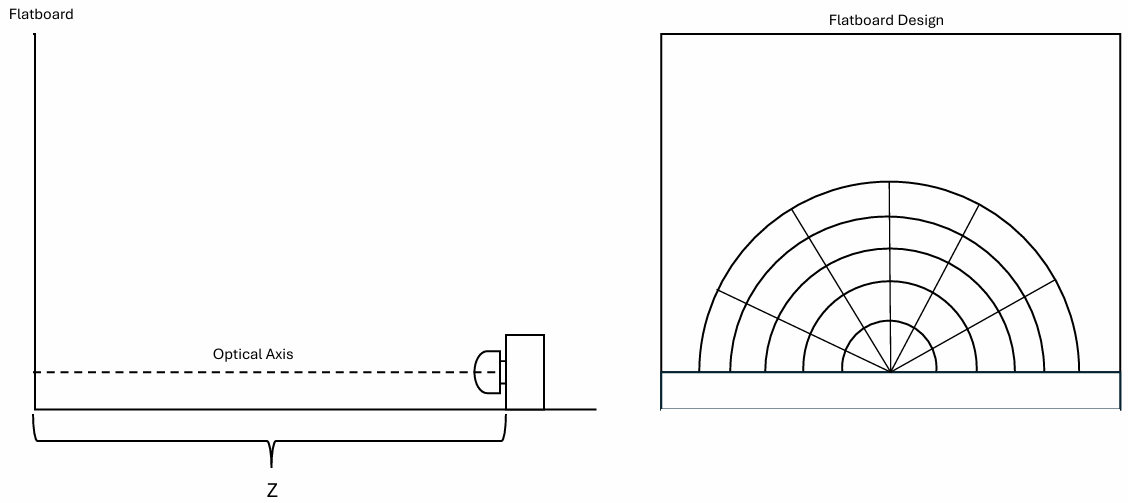
\includegraphics[width=0.75\linewidth]{er_distortion_apparatus.png}
    \caption{Diagram of imaging apparatus used to fit the model described in equations \ref{eq:er_x} to \ref{eq:er_rp}. Diagram courtesy of Ethan Rengifo.}
    \label{fig:er_distortion_apparatus}
\end{figure}

Let $R$ be the radial distance in pixels of a point on the grid projected onto the image plane relative to the projected position of the grid origin (which should be at the center of the image). Let $X$ and $Y$ be the corresponding Cartesian pixel coordinates of the point relative to the projected origin. Let $\phi$ be a coefficient used to determine the offset along $X$ and $Y$.
\begin{align}
    \label{eq:er_x} X &= R \cos(\phi)\\
    \label{eq:er_y} Y &= R \cos(\phi)
\end{align}
Let $\theta$ be the polar angle in radians of the point with respect to the optical axis (i.e., the projected origin of the grid):
\begin{align}
    \label{eq:er_theta} \theta = \arccos\left( \frac{Z}{X^2 + Y^2} \right).
\end{align}
Finally, let $R_p(\theta)$ be the predicted radius of the point in terms of $\theta$:
\begin{align}
    \label{eq:er_rp} R_p (\theta) = f_0 \theta + f_1 \theta^2 + f_2 \theta^4.
\end{align}
Here, $f_0$ should represent the focal length of the lens pixels. The model was fit by comparing the calculated radial distances from the camera images to the true radial distances and minimizing the corresponding $\chi^2$ error, defined as:
\begin{align}
    \chi^2 = \sum_i \frac{(O_i - E_i)^2}{E_i}
\end{align}
where $O_i$ is the observed value and $E_i$ is the expected value.

The fitted parameters were found to be as follows:
\begin{align*}
    x_c &= 639.426 \text{ pixels} \\
    y_c &= 404.388 \text{ pixels} \\
    \phi &= -0.007 \text{ rad} \\ 
    f_0 &= 547.367 \text{ pixels} = 1.642 \text{ mm} \\
    f_1 &= -4.376 \text{ pixels} = -0.013 \text{ mm} \\
    f_2 &= -0.607 \text{ pixels} = -0.002 \text{ mm}
\end{align*}
where $x_c$ and $y_c$ are the pixel coordinates of the optical axis.

\subsection{Magnification from Refractive Surfaces} \label{subsec:magnification_from_refractive_surfaces}
The next source of distortion after a ray exits the camera lenses is the magnification of the image that occurs as the ray travels through the sapphire viewports into the CF$_4$ fluid that has a higher index of refraction than the vacuum the camera sensors are located in. An additional slight magnification occurs as the rays travel through the jars into the LAr fluid. Under the assumption that the cameras have already been calibrated, the additional magnifying distortion caused by these refractive elements can be modeled as a simple linear transformation. Retaining the same variables for $x, y$ and $x', y'$ as in equations \ref{eq:camera_radial_distortion_model_x} and \ref{eq:camera_radial_distortion_model_y}, the linear model is simply:
\begin{align} \label{eq:linear_distortion_mapping}
    x' &= k_0 + k_1 x \\
    y' &= k_2 + k_3 y.
\end{align}
This can be then be set up as the following least squares problem and solved using a pseudo inverse or using QR decomposition, just as in equations \ref{eq:psuedo_inverse} and \ref{eq:QR_decomposition_inverse}:
\begin{align}\label{eq:linear_distortion_model_matrix}
    \begin{bmatrix}
        1 & x_0 & 0 & 0 \\
        0 & 0 & 1 & y_0 \\
        1 & x_1 & 0 & 0 \\
        0 & 0 & 1 & y_1 \\
        \vdots & \vdots & \vdots & \vdots\\
        1 & x_n & 0 & 0 \\
        0 & 0 & 1 & y_n
    \end{bmatrix}
    \begin{bmatrix}
        k_0 \\ k_1 \\ k_2 \\ k_3
    \end{bmatrix}
    =
    \begin{bmatrix}
        x_0' \\ y_0' \\ x_1' \\ y_1' \\ \vdots \\ x_n' \\ y_n'
    \end{bmatrix}.
\end{align}

If we have more data to fit our model to, we can also expand the model by adding polynomial terms:
\begin{align}
    x' &= k_0 + k_1 x + k_2 x^2 + k_3 x^4 \\
    y' &= k_4 + k_5 y + k_6 y^2 + k_7 y^4
\end{align}
which, similar to the linear model, can be expressed and solved as:
\begin{align} \label{eq:polynomial_distortion_model_matrix}
    \begin{bmatrix}
        1 & x_0 & x_0^2 & x_0^4 & 0 & 0 & 0 & 0\\
        0 & 0 & 0 & 0 & 1 & y_0 & y_0^2 & y_0^4\\
        1 & x_1 & x_1^2 & x_1^4 & 0 & 0 & 0 & 0\\
        0 & 0 & 0 & 0 & 1 & y_1 & y_1^2 & y_1^4\\
        \vdots & \vdots & \vdots & \vdots & \vdots & \vdots & \vdots & \vdots\\
        1 & x_n & x_n^2 & x_n^4 & 0 & 0 & 0 & 0\\
        0 & 0 & 0 & 0 & 1 & y_n & y_n^2 & y_n^4
    \end{bmatrix}
    \begin{bmatrix}
        k_0 \\ k_1 \\ k_2 \\ k_3 \\ k_4 \\ k_5 \\ k_6 \\ k_7
    \end{bmatrix}
    =
    \begin{bmatrix}
        x_0' \\ y_0' \\ x_1' \\ y_1' \\ \vdots \\ x_n' \\ y_n'
    \end{bmatrix}.
\end{align}
The \textit{extended} polynomial model takes this even further by adding in coefficients for $x^6, x^8$ and $y^6, y^8$ as well, and can be set up and solved similarly to equations \ref{eq:linear_distortion_model_matrix} and \ref{eq:polynomial_distortion_model_matrix}.

\subsection{Jar Surface Distortions} \label{subsec:jar_surface_distortions}
If the jars were perfectly smooth, we could get decent results with the polynomial model as described above in \S\ref{subsec:magnification_from_refractive_surfaces}. Unfortunately, a large source of distortion, and the one which is hardest to compensate for, is the distortion caused by the `waviness' present in the jar surfaces caused by their manufacturing process. Compared to an ideal jar surface, fitting the extended polynomial model when rendering the simulated distorted jar surface increases the pixel localization error of points from 1.47 pixels up to 1.83 pixels, with the added caveat that the errors are directionally more random (see figure \ref{fig:extended_polynomial_fit_to_ideal_distorted_jar}). Additionally, detecting bubble locations also becomes more difficult as some of the bubbles get distorted to the point where they are no longer detectable with the Hough transform method described in \S\ref{subsec:circle_hough_transform}. The impact of this can also be seen in figure \ref{fig:extended_polynomial_fit_to_ideal_distorted_jar}, as the number of missing remapped points increases when using the ideal jar surface. Note that even when using an ideal jar surface, bubble locations near the edges of the jars also get warped to the point where they are no longer detected by the Hough transform! Determining a better model for remapping points to account for the extra distortions by the jar surfaces unfortunately remains as future work and is discussed more in \S\ref{subsec:future_work}.

\begin{figure}[h]
    \centering
    \subfloat[]{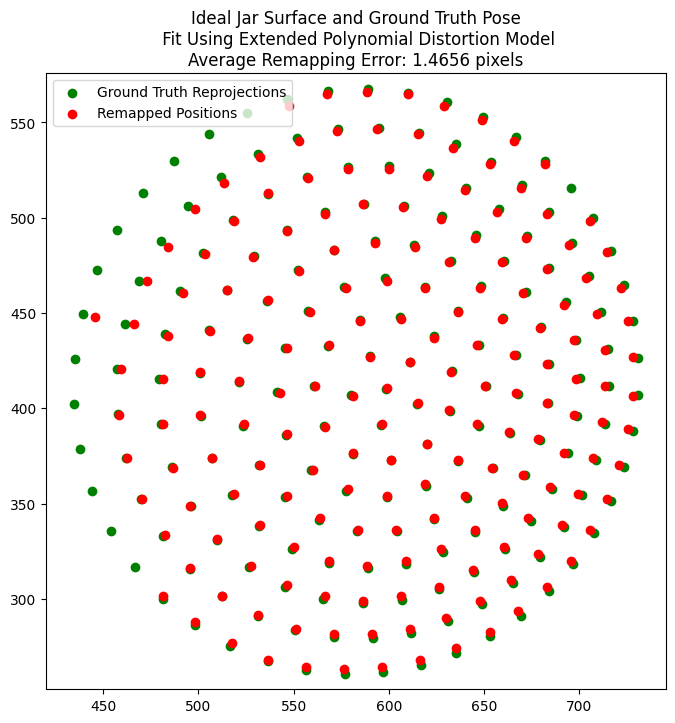
\includegraphics[width=0.45\textwidth]{ideal_jar_surface_fit_using_extended_polynomial_distortion_model.png}}
    \hfill
    \subfloat[]{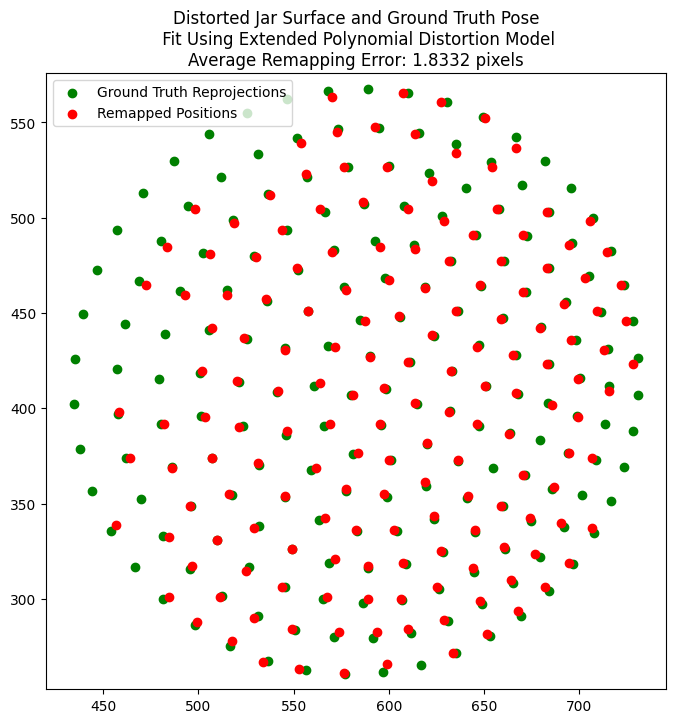
\includegraphics[width=0.45\textwidth]{distorted_jar_surface_fit_using_extended_polynomial_distortion_model.png}}
    \caption{\textbf{(a)} The extended polynomial distortion model fit to renders of the chamber with an ideal jar surface. The distortion coefficients were determined by comparing the calculated positions of bubbles in the renders using OpenCV to the ground truth projections using the known ideal camera matrices and pose matrices. \textbf{(b)} The same model now fit with renders of the distorted jar surface. This shows an increase in pixel remapping error of $25\%$. Green points show the ground truth reprojections of one layer of the testing grid (see figure \ref{fig:testing_grid}) with red points show the corresponding positions of the remapped points. Missing points indicate that OpenCV was unable to determine the location for the grid point.}
    \label{fig:extended_polynomial_fit_to_ideal_distorted_jar}
\end{figure}

\subsection{Impacts of Index of Refraction Errors on Triangulation Accuracy}\label{subsec:impacts_of_index_of_refraction_errors_on_triangulation}
Unaccounted for in the sections above is the uncertainty in the IoRs for the different refractive elements, e.g., errors in the left and right tables of figure \ref{fig:chamber_materials}. Errors in the IoRs would manifest as errors in our remapping functions. Say we determine the coefficients for the extended polynomial model assuming that the IoRs are as stated in figure \ref{fig:chamber_materials} but the true IoRs are off by a few percent. The difference in IoRs would cause rays exiting the camera lenses to curve by different angles due to Snell's law than we would expect with the IoRs used to fit our remapping function, making the remapping function produce erroneous results. 

The following experiment was conducted to determine the relationship between errors in the IoRs and the resulting triangulation errors. For each camera, renders of the chamber were created with the IoRs of the different refractive elements individually changed by a small percentage (in 1\% increments between 95\% of the true value and 105\% of the true value). For each IoR setup, each point of a small grid (as seen in figure \ref{fig:small_testing_grid}) was rendered.\footnote{A smaller grid was used for this test due to the increased number of scenes that needed to be rendered -- one for each change in IoR for each refractive material.} The detected positions of the grid points were then used to fit the extended polynomial model. The resulting distortion coefficients were then used to undistort the ground truth pixel positions with the refractive elements (e.g., the pixel positions with the true IoRs). The average pixel position error compared to the true projected pixel positions (without any refractive surfaces) was calculated for each setup. The resulting charts for pixel localization error and triangulation error as a function of the error in the IoR of each refractive material can be found in figure \ref{fig:effect_of_wrong_iors_on_remapping_and_localization}. The results show a linear relationship between IoR error and triangulation error for the CF4 and LAr, and a negligible relationship for errors in the IoRs of the viewports and jars.

\begin{figure}[h]
    \centering
    \subfloat[]{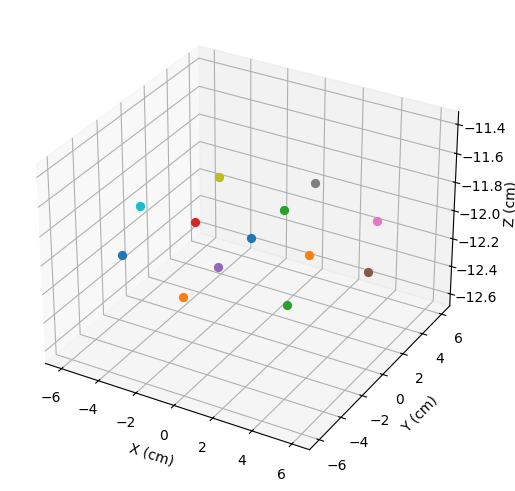
\includegraphics[width=0.4\textwidth]{small_testing_grid_3d.png}}
    \hfill
    \subfloat[]{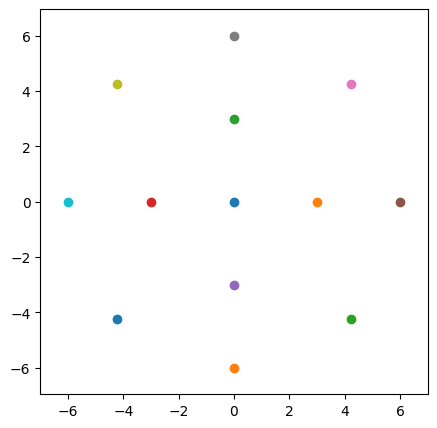
\includegraphics[width=0.4\textwidth]{small_testing_grid_2d.png}}
    \caption{The grid used to test the impact of errors in the IoRs of materials. The size of the grid was significantly reduced to compensate for the increased number of scenes with different IoRs.}
    \label{fig:small_testing_grid}
\end{figure}

\begin{figure}[h]
    \centering
    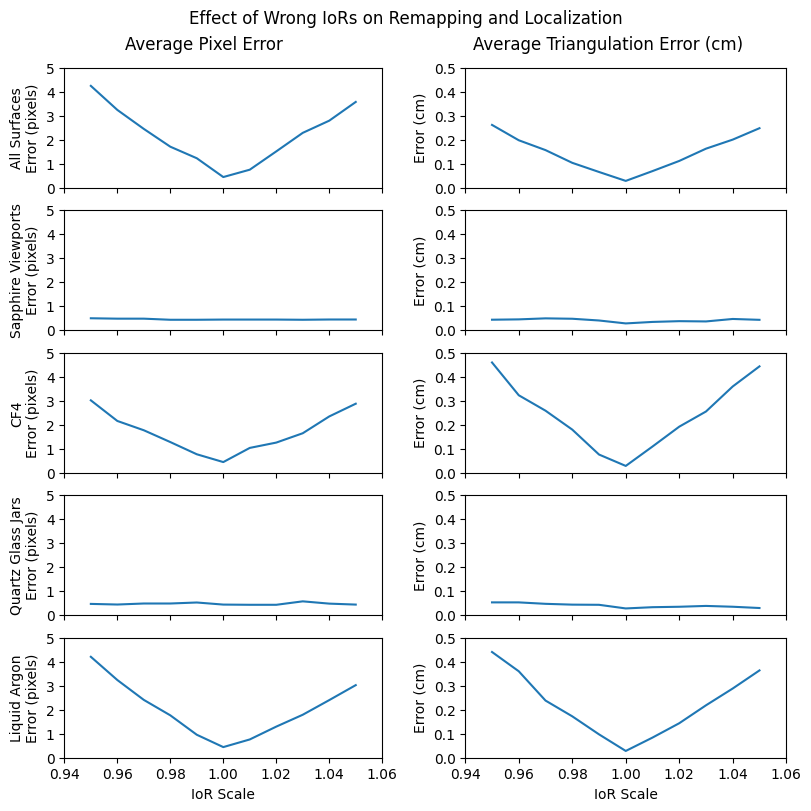
\includegraphics[width=\textwidth]{effect_of_wrong_iors_on_remapping_and_localization.png}
    \caption{Plots showing the average pixel error and the corresponding average triangulation error as a function of the error in the IoR of different refractive elements. The top row is represents the result of changing all IoRs by the same scale factor. The results indicate that changes in the IoRs of the fluids in the chamber (CF4 and LAr) have the largest effect on the triangulation accuracy. While errors in the CF4 IoR produce a smaller pixel error than for errors in LAr, the resulting triangulation error is about the same.}
    \label{fig:effect_of_wrong_iors_on_remapping_and_localization}
\end{figure}

\section{Estimating Camera Parameters} \label{sec:estimating_camera_parameters}
Getting good measurements for the camera parameters is essential for getting high accuracy localizations of the bubbles. In the following subsections, we will cover how these parameters can be calculated for rendered and real images.

\subsection{The Camera Matrix} \label{subsec:the_camera_matrix}
In the ideal case, the camera matrix can be manually calculated given the field of view \footnote{The field of view for these equations is represented in radians to make the equations more concise. In practice, Mitsuba takes in degrees so the functions in our code also convert degrees to radians before performing calculations.} ($\text{fov}$), the axis along which the field of view is defined (i.e., the `$x$' or `$y$' axis), the image dimensions in pixels ($p_x, p_y$), and the physical sensor dimensions ($s_x, s_y$). The general relationship between the field of view along a given axis, the size of the sensor along that axis, and the focal length along that axis ($f$) is given by:
\begin{align}\label{eq:fov_wrt_s&f}
    \text{fov} = 2 \arctan \left( \frac{s}{2f} \right).
\end{align}
We can also solve the above equation for the focal length in terms of the field of view and the sensor size:
\begin{align}\label{eq:f_wrt_s&fov}
    f = \frac{s}{2 \tan \left( \frac{\text{fov}}{2} \right)}.
\end{align}
Using equation \ref{eq:f_wrt_s&fov}, we can calculate the ideal camera matrix as:
\begin{align}
    K =
    \begin{bmatrix}
        \frac{s_j}{2 \tan \left( \frac{\text{fov}_j}{2} \right)} \frac{p_j}{s_j} & 0 & \frac{p_x}{2} \\
        0 & \frac{s_j}{2 \tan \left( \frac{\text{fov}_j}{2} \right)} \frac{p_j}{s_j} & \frac{p_y}{2} \\
        0 & 0 & 1
    \end{bmatrix}
    =
    \begin{bmatrix}
        \frac{p_j}{2 \tan \left( \frac{\text{fov}_j}{2} \right)} & 0 & \frac{p_x}{2} \\
        0 & \frac{p_j}{2 \tan \left( \frac{\text{fov}_j}{2} \right)} & \frac{p_y}{2} \\
        0 & 0 & 1
    \end{bmatrix}
\end{align}
where $j$ is a stand in for either $x$ or $y$. We scale the focal lengths to be in pixel units by dividing by the physical size of each pixel (i.e., multiply by $p_j/s_j$) which allows the camera matrix to be independent of the physical sensor size. Also, note how in the ideal case, the focal lengths $f_x$ and $f_y$ are identical which is not necessarily true in reality.

For actual cameras, the camera matrix can be calculated as part of the camera calibration process as described in \S\ref{subsec:camera_calibration}.
% (When running camera calibration on rendered images, we can get near-exact results for the focal lengths and centers of the simulated cameras...)

\subsection{The Pose Matrix} \label{subsec:the_pose_matrix}
Computing the pose matrix $V$ for a particular camera requires that we know already know the camera matrix $K$, and the real-world coordinates $\mathbf{w}$ and corresponding projected pixel positions $\mathbf{p}$ of a set of scene points. The 12 unknowns that compose the pose matrix $V$ can then be solved using a set of techniques known as Perspective-n-Point (PnP) algorithms. At the least, PnP requires 3 coplanar, or 4 non-coplanar point correspondences to be present in an image to compute the pose of the camera. Luckily, for the SBC chambers, each of the three cameras has in its field of view, a set of \textit{5} coplanar fiducial markers whose 3D positions are known within $\pm 0.1$ cm. 

In the code, the camera matrices and distortion coefficients along with the 5 fiducial marker positions and their corresponding image projections in pixel coordinates are passed into OpenCV's \verb|solvePnP| function. By default, this function uses a LM-based iterative optimization approach by minimizing the reprojection errors of the scene points, just like is described in \S\ref{subsec:levenberg-marquardt}. To initialize the optimization for planar points like in our case, the function performs a homography decomposition. For more details on the PnP algorithm provided by OpenCV and used in the code, readers are directed to the OpenCV documentation \cite{opencv_library}. 

The function returns a 3-element translation vector and a 3-element rotation vector. The rotation vector is an axis-angle representation of the rotation with the direction of the vector representing an axis of rotation and the magnitude of the vector representing the amount of rotation about that axis in radians. The rotation vector can be converted to the desired rotation matrix $R \in \mathbb{R}^{3 \times 3}$ using the \textit{Rodrigues} formula, which is also a built-in function in OpenCV. 

Note that the returned translation vector and rotation vector converted to a rotation matrix represent the \textit{object pose}, not the camera pose. I.e., they assume the camera is the origin of the coordinate system and the pose matrix moves the object relative to the camera. If we instead want to get the \textit{camera pose}, we can concatenate the translation vector to the rotation matrix (just as in equation \ref{eq:camera_intrinsic_extrinsic}), then convert that $3 \times 4$ matrix into a $4 \times 4$ matrix by adding a row with values $[0, 0, 0, 1]$ and invert it. The first three rows of that inverted matrix are then the \textit{camera's} pose matrix.

Additionally, if we want the produced pose matrix to match the pose matrices that we can derive from Mitsuba (i.e., the camera's `to\_world' matrix), we need to pre-multiply the rotation matrix and translation vector by a $3 \times 3$ rotation matrix $z_{\text{flip}}$ (see equation \ref{eq:z_flip}) that performs a 180 degree rotation along the z-axis. This is necessary because Mitsuba uses a left-handed coordinate system while the returned rotation and translation vectors assume a right-handed coordinate system for the camera. See the function \verb|switch_handedness| in the code for implementation details.
\begin{align}\label{eq:z_flip}
    z_{\text{flip}} =
    \begin{bmatrix}
        -1 &  0 &  0 \\
         0 & -1 &  0 \\
         0 &  0 &  1
    \end{bmatrix}
\end{align}

To test the impact of errors in pose estimation on localization, the pose matrix for each camera in the renders was estimated using the PnP method described above. First, a render was made for each camera and the pixel positions of the fiducial markers in the renders was estimated by hand.\footnote{At most, the estimated fiducial marker positions used to estimate the pose for figure \ref{fig:PnP_error_estimated_poses} were off by no more than 2 pixels.} Then, those pixel positions and the real world coordinates of the fiducial markers (taken from the corresponding Blender model) were plugged into OpenCVs \verb|solvePnP| function whose outputs were used to compute the pose matrices (see the function \verb|estimate_pose_matrix| for more details). 

The resulting pose matrices had camera position errors of $0.564, 0.816$ and $0.440$ cm when compared to the true pose matrices determined by extracting the \verb|to_world| matrix of the rendered cameras. The errors in rotation were calculated by determining the cosine angle between the rotation matrices. For rotation matrices $P$ and $Q$, the \textit{difference rotation matrix} can be defined as $R = P Q^T$ and the trace of the difference rotation matrix can be used to determine the cosine angle \cite{trefethen2022numerical}:
\begin{align}
    \mathrm{trace}(R) &= 1 + 2 \cos(\theta) \\
    \theta &= \arccos \left(\frac{\mathrm{trace}(R)-1}{2} \right).
\end{align}
Using this metric, the error in rotation for the camera poses was found to be $1.574, 1.898,$ and $1.201$ degrees.

To compute the error in triangulation, the grid points as in figure \ref{fig:testing_grid} were directly projected onto the camera plane using the \textit{actual} pose matrices. Then, those projected grid points were passed into the \verb|n_view_triangulate| function with the \textit{estimated} pose matrices to simulate the error in triangulation when there is a disparity between the true and estimated poses. Since these points were directly projected onto the image planes, the only sources of error in the resulting triangulations must be due to the error in the pose. The resulting average error for the grid points came out to be $0.208$ cm (see figure \ref{fig:PnP_error_estimated_poses}).

\begin{figure}[h]
    \centering
    \subfloat{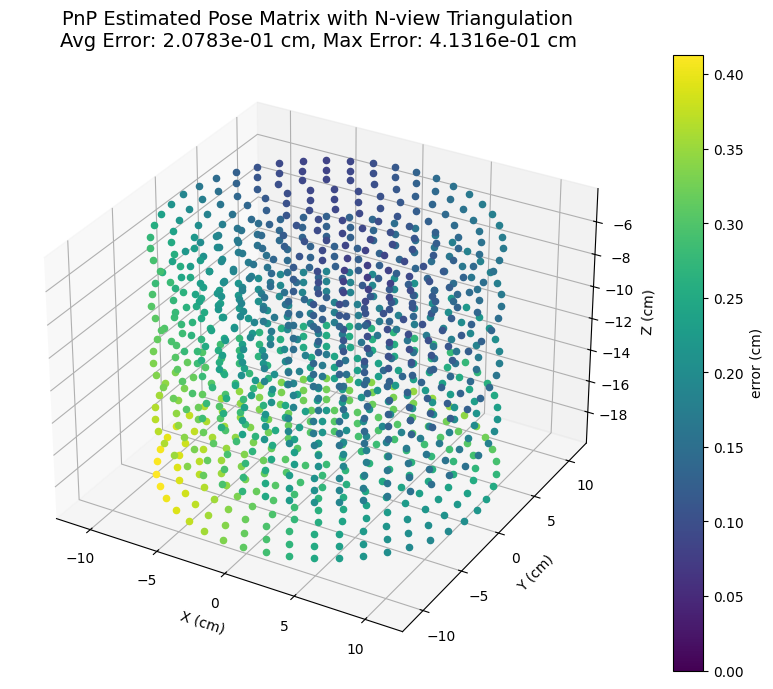
\includegraphics[height=1.75in]{PnP_pose_estimate_triangulation_error_grid.png}}
    \hfill
    \subfloat{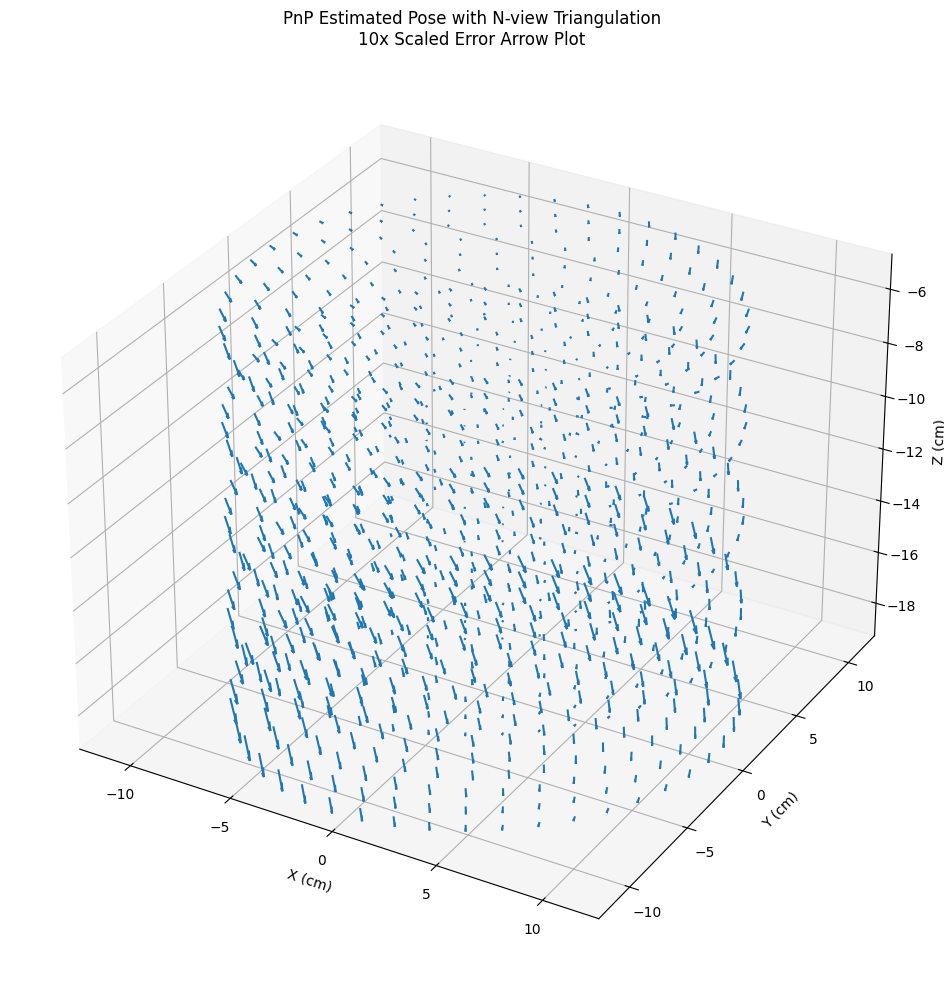
\includegraphics[height=1.75in]{PnP_pose_estimate_triangulation_arrow_plot.png}}
    \hfill
    \subfloat{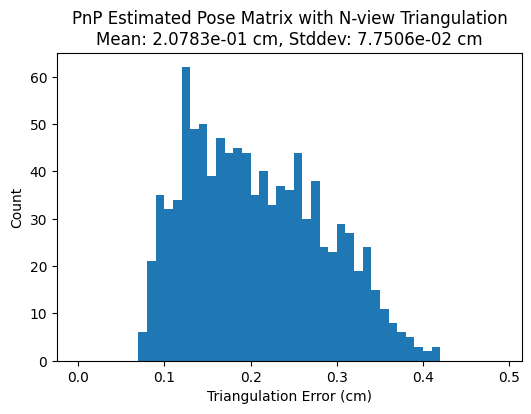
\includegraphics[height=1.75in]{PnP_pose_estimate_triangulation_histogram.png}}
    \caption{\textit{(Left)} Color plot of triangulation error using PnP-estimated pose matrices. \textit{(Center)} Corresponding arrow plot of triangulation errors. Arrow tails are true positions of the grid points, heads are the triangulated positions. Note, the lengths of the arrows have been scaled up by a factor of 10 to better show error direction. \textit{(Right)} Histogram of triangulation error in centimeters.}
    \label{fig:PnP_error_estimated_poses}
\end{figure}

Additional testing was done to determine the impact of fiducial marker pixel localization error on pose estimation and consequently, on triangulation. This time, the exact fiducial marker positions were projected onto the camera sensors using their actual pose matrices. Then, the pose matrices for each camera were estimated after offsetting the fiducial markers pixel positions within some random circle of a given pixel radius. The grid of points was then triangulated using those estimated pose matrices and the average errors were recorded. This was done for several sizes of random pixel offsets. See figure \ref{fig:PnP_error_pixel_offset} for the results of these tests which indicate linear relationships between the pixel error of the fiducial markers and the corresponding error in pose estimation and triangulation.

\begin{figure}[h]
    \centering
    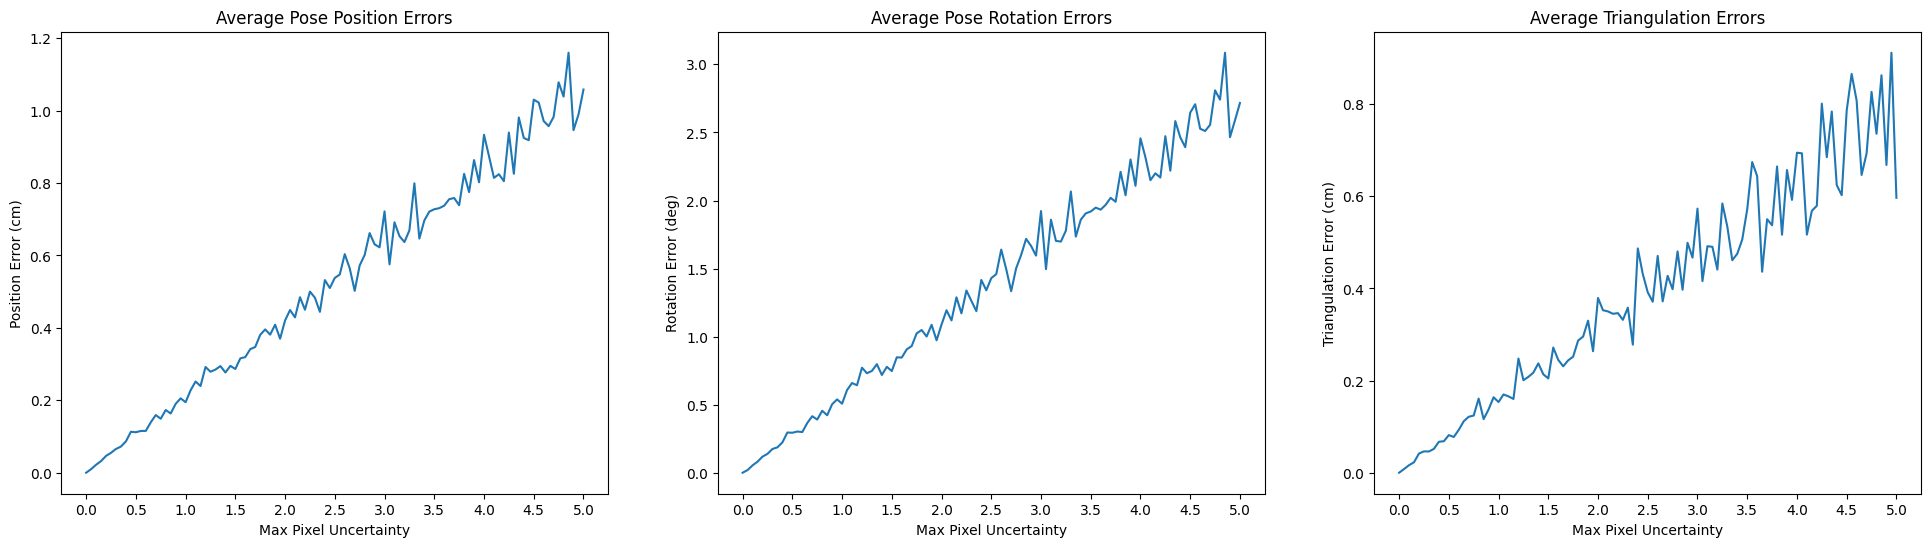
\includegraphics[width=\textwidth]{PnP_pixel_offset_errors.png}
    \caption{These plots show the effect that pixel localization errors of the fiducial markers have on the errors in the estimated pose matrices and the corresponding triangulation errors. These plots were calculated by estimating the pose matrices with varying amounts of uncertainty in the pixel positions of each fiducial marker (represented by the x-axis) and using those estimated pose matrices to triangulate the grid of points as shown in figure \ref{fig:testing_grid}. At each amount of uncertainty in pixel position, the average error in the position of the camera in cm (left), the average error in the rotation of the camera in degrees (middle), and the average triangulation error of grid points in cm (right) was taken over several randomized runs. The results show a roughly linear relationship between pixel error and the corresponding pose error and triangulation errors.}
    \label{fig:PnP_error_pixel_offset}
\end{figure}


\section{Bubble Triangulation} \label{sec:bubble_triangulation}
Once we know the undistorted pixel positions of corresponding bubbles across images, each of the cameras' pose matrices, and intrinsic camera matrices, we can determine the ray origins and directions of the corresponding rays from each camera in the direction of a given bubble as described in equations \ref{eq:ray_origin} and \ref{eq:ray_direction}. From these rays, we can determine the point of closest intersection using one of two methods presented below to provide an initial estimate of the position of the bubble. This result can be further optimized using the strategies presented in \S\ref{sec:optimization_techniques}. A discussion of the performance of the two triangulation methods can be found in \S\ref{subsec:comparison_of_triangulation_methods}.

\subsection{Mid-Point Two View Triangulation} \label{subsec:mid-point_two_view_triangulation}
The first method triangulates the position of the bubble using each pair of cameras and then takes the average of the triangulated position to provide our initial estimate. For each pair of rays, the point of closest intersection $H$ can be determined by finding the location of the bisecting point of the vector $\overrightarrow{FG} = G - F$ (where $G = Q + \mu \bar{s}$ and $F = P + \lambda \bar{r}$) which is orthogonal to both direction vectors $\bar{r}$ and $\bar{s}$ (see figure \ref{fig:mid-point_two_view_triangulation}).

\begin{figure}[h!]
    \centering
    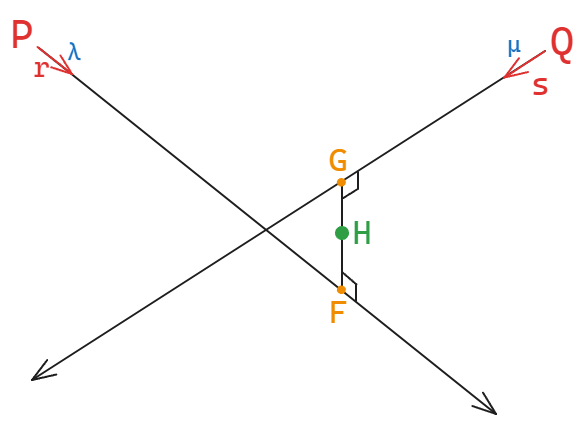
\includegraphics[width=0.6\linewidth]{midpoint_two_view_triangulate.png}
    \caption{The point of closest intersection $H$ between two rays can be determined by finding the bisecting point of the vector $\overrightarrow{FG}$ which is orthogonal to both direction vectors $\bar{r}$ and $\bar{s}$.}
    \label{fig:mid-point_two_view_triangulation}
\end{figure}

This constraint can be expressed as:
\begin{align*}
    (G - F) \cdot \bar{r} &= 0 \\
    (G - F) \cdot \bar{s} &= 0.
\end{align*}
Expanding this, we get:
\begin{align*}
    (Q + \mu \bar{s} - P - \lambda \bar{r}) \cdot \bar{r} &= 0 \\
    (Q + \mu \bar{s} - P - \lambda \bar{r}) \cdot \bar{s} &= 0,
\end{align*}
which can be factored into:
\begin{align*}
    (Q - P)^T \bar{r} + \mu \bar{s}^T \bar{r} - \lambda \bar{r}^T \bar{r} &= 0 \\
    (Q - P)^T \bar{s} + \mu \bar{s}^T \bar{s} - \lambda \bar{r}^T \bar{s} &= 0,
\end{align*}
and rearranged as:
\begin{align*}
    (Q - P)^T \bar{r} &= \lambda \bar{r}^T \bar{r} - \mu \bar{s}^T \bar{r} \\
    (Q - P)^T \bar{s} &= \lambda \bar{r}^T \bar{s} - \mu \bar{s}^T \bar{s}.
\end{align*}
Expressing this in matrix form, we get:
\begin{align*}
    \begin{bmatrix}
    (Q - P)^T \bar{r}\\
    (Q - P)^T \bar{s}
    \end{bmatrix}
    &=
    \begin{bmatrix}
    \bar{r}^T \bar{r} & -\bar{s}^T \bar{r} \\
    \bar{r}^T \bar{s} & -\bar{s}^T \bar{s}
    \end{bmatrix}.
\end{align*}
We can solve for the coefficients $\lambda$ and $\mu$ which represent the distance along along each ray required to reach points $G$ and $F$:
\begin{align}
    \begin{bmatrix}
    \lambda \\ 
    \mu
    \end{bmatrix}
    =
    \begin{bmatrix}
    \bar{r}^T \bar{r} & -\bar{s}^T \bar{r} \\
    \bar{r}^T \bar{s} & -\bar{s}^T \bar{s}
    \end{bmatrix}^{-1}
    \begin{bmatrix}
    (Q - P)^T \bar{r} \\
    (Q - P)^T \bar{s}
    \end{bmatrix}.
\end{align}
Once we have these coefficients, we can finally solve for our desired bisecting point $H$:
\begin{align} \label{eq:midpoint_two_view_H}
    H = F + (G - F)/2 = \frac{F + G}{2} = \frac{P + \lambda \bar{r} + Q + \mu \bar{s}}{2}.
\end{align}
Doing this calculation with the corresponding rays from each pair of cameras, we can determine the average of the calculated midpoints to get our initial estimate.

\subsection{N-view Triangulation with Least Squares} \label{subsec:n-view_triangulation_with_least_squares}
The other triangulation method uses least squares to determine a point $\mathbf{p}$ which minimizes the projected distances onto all three camera rays simultaneously (see figure \ref{fig:n-view_triangulate}). One additional benefit of this method, which is not taken advantage of here, is that it generalizes to any number of cameras, as long as we have the relevant camera and pose matrices for each and the undistorted pixel location of the feature to triangulate. 

\begin{figure}[h!]
    \centering
    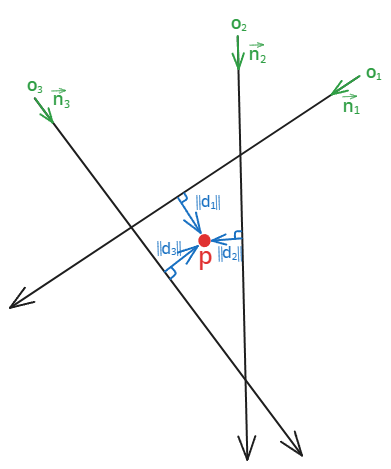
\includegraphics[width=0.4\linewidth]{n-view_triangulate.png}
    \caption{N-view triangulation determines a position $\mathbf{p}$ which minimizes the sum of projected distances to the camera rays $\sum_i d_i$.}
    \label{fig:n-view_triangulate}
\end{figure}

Let $\mathbf{o}_i$ be the origin of ray $i$. Let $\mathbf{n}_i$ be the \textit{unit} direction vector for ray $i$. Let $\mathbf{p}$ be the closest point of intersection for all rays. The closest distance $d_i$ of ray $i$ to point $\mathbf{p}$ is: 
\[
    d_i = ||(\mathbf{p}-\mathbf{o}_i) \times \mathbf{n}_i||.
\]
Using the identity
\[
(\mathbf{a} \times \mathbf{b})\cdot(\mathbf{a} \times \mathbf{b}) = ||\mathbf{a}||^2 ||\mathbf{b}||^2 - (\mathbf{a} \cdot \mathbf{b})^2,
\]
we can re-express $d_i$ as:
\begin{align*}
    d_i^2 &= ||\mathbf{p}-\mathbf{o}_i||^2 ||\mathbf{n}_i||^2 - \left((\mathbf{p}-\mathbf{o}_i) \cdot \mathbf{n}_i\right)^2 \\
          &= ||\mathbf{p}-\mathbf{o}_i||^2 - \left((\mathbf{p}-\mathbf{o}_i) \cdot \mathbf{n}_i\right)^2.
\end{align*}
Now, our objective is to find $\mathbf{p}$ such that the sum $\sum_i d_i^2$ for all rays is minimized. We know the point where that sum is minimized should have a derivative of $0$ with respect to the position of the point $\mathbf{p}$, so we can evaluate the derivative of $d_i^2$ with respect to the position of point $\mathbf{p}$:
\[
\frac{\partial (d_i^2)}{\partial \mathbf{p}} = 2 ||\mathbf{p} - \mathbf{o}_i|| - 2||\mathbf{n}_i \left( (\mathbf{p} - \mathbf{o}_i) \cdot \mathbf{n}_i \right)||.
\]
Setting the derivative to 0, we get:
\begin{align*}
    0 &= ||\mathbf{p} - \mathbf{o}_i|| - ||\mathbf{n}_i \left( (\mathbf{p} - \mathbf{o}_i) \cdot \mathbf{n}_i \right)|| \\
    \mathbf{p} - \mathbf{o}_i &= \mathbf{n}_i \left( (\mathbf{p} - \mathbf{o}_i) \cdot \mathbf{n}_i \right) \\
    (\mathbf{p} - \mathbf{o}_i) &= (\mathbf{n}_i \mathbf{n}_i^T)(\mathbf{p} - \mathbf{o}_i).
\end{align*}
Let $a = \mathbf{p}$, let $b = \mathbf{o}_i$, and let $\mathbf{c}  = \mathbf{n}_i \mathbf{n_i}^T$. Then we can refactor the above as:
\begin{align*}
    (a-b) &= \mathbf{c}(a-b) \\
    0 &= \mathbf{c}(a-b) - (a-b) \\
    0 &= \mathbf{c}a - \mathbf{c}b - a + b \\
    0 &= (\mathbf{c} - \mathbf{I}) (a - b) \\
    (\mathbf{c} - \mathbf{I})a &= (\mathbf{c} - \mathbf{I})b.
\end{align*}
Plugging in the original values for $a, b, \mathbf{c}$ and making it a sum over all views, we can express this as the following least squares problem that we can solve using a pseudo-inverse:
\begin{align}
    \left[ \sum_i \left(\mathbf{n}_i \mathbf{n}_i^T - \mathbf{I}\right) \right] \mathbf{p} &= \left[ \sum_i \left(\mathbf{n}_i \mathbf{n}_i^T - \mathbf{I}\right) \mathbf{o}_i \right] \\
    A \mathbf{p} &= \mathbf{b} \\
    \mathbf{p} &= (A^T A)^{-1}A^T \mathbf{b}.
\end{align}

\subsection{Comparison of Triangulation Methods}\label{subsec:comparison_of_triangulation_methods}
Testing has shown the N-view triangulation method shown in \S\ref{subsec:n-view_triangulation_with_least_squares} to outperform the average of mid-point two view method as shown in \S\ref{subsec:mid-point_two_view_triangulation}, likely because it optimizes the result over all three views simultaneously. For example, if we use the exact reprojections of the grid points in figure \ref{fig:testing_grid} onto the camera sensors, the resulting average error when computing the triangulation with the average of mid-point two view triangulations is $5.6634 \times 10^{-8}$ cm. Using the n-view triangulation method however, results in an average error of just $2.839 \times 10^{-14}$ cm, which is low enough to be influenced by floating point precision errors in the arithmetic.

In practice however, the accuracy boost in triangulation error can be fairly minor. For example, when testing the localization error for rendered images using the true pose matrices and ideal jar surfaces with a linear remapping coefficients, using mid-point two view resulted in an average error of $0.1273$ cm, but using n-view only improved the average error down to $0.1258$ cm, an improvement of just $1.1\%$.


\section{Optimization Techniques} \label{sec:optimization_techniques}
Once we have an initial estimate for the bubble position, we can improve the result by performing an optimization which minimizes the cumulative reprojection error for all three cameras. Testing has shown that these optimizations have a relatively minor impact on triangulation accuracy for this application and can even slightly worsen triangulation results if pixel localizations are bad (see \S\ref{subsec:comparison_of_optimizations}), but the following section is kept for completeness. As in \cite{hedborg2014robust}, we formulate the cumulative reprojection errors as the following loss function. Let $P_1, P_2, P_3 \in \mathbb{R}^{3 \times 4}$ be the projection matrices for each of the cameras (where each projection matrix is the product of the corresponding camera matrix $K$ and pose matrix $V$ as seen in equation \ref{eq:camera_intrinsic_extrinsic}), and let $\mathbf{x}_1, \mathbf{x}_2, \mathbf{x_3} \in \mathbb{R}^{2}$ be the corresponding image projections of a scene point $\mathbf{w} \in \mathbb{R}^3$ and with $\mathbf{w}^h \in \mathbb{R}^4$ being the homogeneous representation of $\mathbf{w}$. The image residual for one reprojection $i$ can then be defined as
\begin{align}
    \mathbf{r}_i = \mathbf{x}_i - \mathrm{proj}(P_i \mathbf{w}^h)
\end{align}
where the projection mapping $\mathrm{proj}() \in \mathbb{R}^3 \rightarrow \mathbb{R}^2$ is defined as 
\begin{align}
    \mathrm{proj}(\mathbf{y}) = \begin{bmatrix} \frac{y_1}{y_3} & \frac{y_2}{y_3} \end{bmatrix}^T.
\end{align}
We want to find the position of the 3D point $\mathbf{w}$ such that 
\begin{align}
    f = ||\mathbf{r}||^2_2, \; \mathbf{r} = \begin{bmatrix} r_{1x} & r_{1y} & \cdots & r_{3x} & r_{3y} \end{bmatrix}^T
\end{align}
is minimized. This can be achieved using a variety of non-linear optimization methods. The simplest method is gradient descent which is described in \S\ref{subsec:gradient_descent}. However, a more common approach in computer vision is to use Levenberg-Marquardt as described in \S\ref{subsec:levenberg-marquardt}. In the following sections, we will cover the basic theoretical bases of these algorithms. We will also discuss how these algorithms are implemented numerically. Since there is no explicit representation of the loss function $f(\mathbf{w})$ for which we can compute the first and second order derivatives, those need to be computed numerically at each optimization step. Finally, we also showcase the convergence performance of the different techniques. For a more thorough discussion of optimization techniques, the reader is directed to \cite{madsen2004methods}. 

\subsection{Gradient Descent}\label{subsec:gradient_descent}
\textit{Gradient descent} (GD), also known as \textit{steepest descent} is among the simplest optimization techniques available as it simply moves the predicted point in the direction that minimizes the loss function at each optimization step. The usual formulation for GD is as follows. Given a current prediction $\mathbf{x}_i$, the gradient of the loss function at that prediction $\nabla f(\mathbf{x}_i)$, and a step size scaling factor $\lambda_i$, the updated prediction $\mathbf{x}_{i+1}$ is given by:
\begin{align} \label{eq:gradient_descent}
    \mathbf{x}_{i+1} = \mathbf{x}_i - \lambda_i \nabla f(\mathbf{x}_i)
\end{align}

However, GD has a number of drawbacks. If we follow the formulation in equation \ref{eq:gradient_descent}, if $f(\mathbf{x})$ is relatively flat, the step size will be very small. If the gradient is instead large, we are likely to overshoot the minimum. Another common limitation of this method is its tendency to get stuck in \textit{local} minima as the basic versions of this method have no utility to take a large enough step to exit a local minima. Its convergence can also be slow for loss landscapes that feature a valley-like structure, causing the optimization to zig-zag between the walls of the valley. A common improvement to gradient descent is to add some way of scaling $\lambda_i$ so that larger steps are taken at the start of optimization and progressively smaller steps are taken later in optimization as we approach the minimum. This could be as simple as reducing the step size as a function of the current optimization step which is the approach used in our code. More advanced versions of gradient descent exist in the literature including stochastic gradient descent and gradient descent with momentum which aim to improve its convergence properties but those are not covered in this paper.

The most basic GD algorithm implemented in the code uses a fixed $\delta$ set by the user and does not compute the true gradient. Instead, at each iteration step, the loss function is evaluated at the current predicted location plus the $\delta$ along each of the 6 cardinal directions $[\pm \delta \hat{x}, \pm \delta \hat{y}, \pm \delta \hat{z}]$.\footnote{In the figure below, this GD method is identified as `Basic Gradient Descent' as opposed to `Gradient Descent' which actually computes the interpolated gradient along all dimensions simultaneously.} Then, the predicted location is updated with the direction that has the minimum in the loss. Optionally, the user can choose to scale the size of the $\delta$ by the remaining number of iterations. So on iteration $i$ of $n$ total iterations, the step size $\delta_i$ is determined by
\begin{align}
    \delta_i = \delta \left(\frac{n-i}{n} \right).    
\end{align}
The major drawback of this method is that the accuracy is limited by the chosen size of the $\delta$. If the $\delta$ scaling is disabled, the result will zig-zag around the loss minimum without converging. It scaling is enabled, the result will still zig-zag but should get closer to the optimal result, though it will still be limited by the minimum scale factor used.

The usual GD algorithm as it is represented in equation \ref{eq:gradient_descent} is also implemented in the code. At each step, the gradient $\nabla f (\mathbf{x})$ is computed numerically using a step size $h$:\footnote{Methods for evaluating derivatives using small step sizes like this are known in the literature as \textit{finite difference methods} and there are a variety of methods used in practice. The methods proposed in this paper are \textit{central difference methods}.}
\begin{align}
    \nabla f(\mathbf{x}) = 
    \begin{bmatrix}
    \frac{f (\mathbf{x} + h \hat{x}) - f(\mathbf{x} - h \hat{x})}{2 h} \\
    \frac{f (\mathbf{x} + h \hat{y}) - f(\mathbf{x} - h \hat{y})}{2 h} \\
    \frac{f (\mathbf{x} + h \hat{z}) - f(\mathbf{x} - h \hat{z})}{2 h}
    \end{bmatrix}
\end{align}
and updates are performed as expressed in equation \ref{eq:gradient_descent}. As stated earlier, the major draw back of this method is that convergence slows as we approach the minimum, requiring an increase in the number of iterations.

\subsection{Newton-Raphson}\label{subsec:newton-raphson}
The \textit{Newton-Raphson} (NR) method takes into account the curvature of the function as well, expressed by the function's \textit{Hessian matrix} which is the matrix of second order partial derivatives: $\nabla^2 f(\mathbf{x}_n)$. See \S\ref{subsubsec:hessian_matrix} for its formulation and numerical computation. An iteration with NR can be expressed as:
\begin{align} \label{eq:newton-raphson}
    \mathbf{x}_{i+1} = \mathbf{x}_i - \left( \nabla^2 f(\mathbf{x}_i) \right)^{-1} \; \nabla f(\mathbf{x}_i).
\end{align}
Generally, the NR method is faster to converge than GD because it can travel farther in areas that have low curvature (are relatively flat) and travel slower in areas of large curvature, making it less likely to overshoot. However, it has its own drawbacks. First, computing the Hessian can be expensive when we do not have a defined $f(\mathbf{x})$ and it is made worse since we need to compute its inverse which can be expensive if the Hessian matrix is large (i.e., $\mathbf{x}$ is high dimensional). Also, it might not be possible to invert the Hessian, especially if the Hessian is singular (its determinant is 0). This is where floating point precision errors come in to play, especially if the determinant is very small -- thus requiring high floating point precision for stability. Additionally, if the Hessian is not positive definite, then NR will not lead to the minimum, instead causing it to `wander around', get stuck in a cycle, or even diverge. Finally, it is very likely to get stuck in local minima and therefore requires good initialization.

\subsubsection{Hessian Matrix}\label{subsubsec:hessian_matrix}
The Hessian matrix for a function $f(\mathbf{x}) \in \mathbb{R}^d$ can be expressed as:
    \begin{align}
    \mathbf{H} = \nabla^2 f(\mathbf{x}) = 
    \begin{bmatrix}
    \frac{\partial^2 f}{\partial x_1^2} & \frac{\partial^2 f}{\partial x_1 \partial x_2} & \cdots & \frac{\partial^2 f}{\partial x_1 \partial x_d} \\
    \frac{\partial^2 f}{\partial x_2 \partial x_1} & \frac{\partial^2 f}{\partial x_2^2} & \cdots & \frac{\partial^2 f}{\partial x_2 \partial x_d} \\
    \vdots & \vdots & \ddots & \vdots \\
    \frac{\partial^2 f}{\partial x_d \partial x_1} & \frac{\partial^2 f}{\partial x_d \partial x_2} & \cdots & \frac{\partial^2 f}{\partial x_d^2} \\
    \end{bmatrix}
    =
    \begin{bmatrix}
    \frac{\partial \overrightarrow{\nabla}f}{\partial x_1} \\
    \frac{\partial \overrightarrow{\nabla}f}{\partial x_2} \\
    \vdots \\
    \frac{\partial \overrightarrow{\nabla}f}{\partial x_d}
    \end{bmatrix}
\end{align}
where
\begin{align}
    \overrightarrow{\nabla} f = \begin{bmatrix} \frac{\partial f}{\partial x_1} & \frac{\partial f}{\partial x_2} & \cdots & \frac{\partial f}{\partial x_d} \end{bmatrix}.
\end{align}
Note that this matrix is symmetric about the diagonal. E.g, $\frac{\partial^2 f}{\partial x_1 \partial x_2} = \frac{\partial^2 f}{\partial x_2 \partial x_1}$. Therefore, we only need to compute $\frac{n^2 - n}{2}$ elements (instead of the full $n^2$ elements). Also, we can solve for $\overrightarrow{\nabla}f$ once and compute the partial derivatives after to further speed things up.

In our code, the Hessian matrix is computed numerically such that element $H_{ij}$ of the Hessian is equal to:
\begin{align}\label{eq:hessian_element}
    H_{ij} = \frac{f(\mathbf{x} + h \hat{e}_i + h \hat{e}_j) - f(\mathbf{x} - h \hat{e}_i + h \hat{e}_j) - f(\mathbf{x} + h \hat{e}_i - h \hat{e}_j) + f(\mathbf{x} - h \hat{e}_i - h \hat{e}_j)}{4h^2}
\end{align}
so that for 3 dimensions,
\begin{align}
    \nabla^2 f(\mathbf{x}) = \mathbf{H} = 
    \begin{bmatrix}
    H_{xx} & H_{xy} & H_{xz} \\
    H_{yx} & H_{yy} & H_{yz} \\
    H_{zx} & H_{zy} & H_{zz} 
    \end{bmatrix}.
\end{align}
Note that in this implementation, we are not taking advantage of the ability to just compute $\overrightarrow{\nabla}f$ once but we do set $H_{yx} = H_{xy}, H_{zx} = H_{xz}$, and $H_{zy} = H_{yz}$. For our application, since we are doing offline analysis, the extra optimization was skipped for now. Though, it should be a relatively simple adjustment to equation \ref{eq:hessian_element}.

\subsection{Levenberg-Marquardt}\label{subsec:levenberg-marquardt}
The Levenberg-Marquardt algorithm combines GD and NR. An update using LM can be expressed as:
\begin{align}
    \mathbf{x}_{i+1} = \mathbf{x}_i - \left( \nabla^2 f(\mathbf{x}_i) + \lambda \mathbf{I} \right)^{-1} \; \nabla f(\mathbf{x}_i).
\end{align}

When $\lambda \rightarrow 0$, the LM method approaches NR, and when $\lambda \rightarrow \infty$, it approaches GD with small steps. If $\lambda$ is sufficiently large, even if the Hessian matrix is not positive definite, the matrix $\mathbf{H} + \lambda \mathbf{I}$ can be positive definite and thus guarantees a reduction in the function's value.

To improve the LM algorithm, if in each step of the update, the cost function goes down (which implies that the curvature is helping), we accept the step and reduce $\lambda$ (by a factor of 2 in the code) to reduce the influence of gradient descent. On the other hand, if the cost function goes up, we retract the step and increase $\lambda$ (by a corresponding factor of 2).\footnote{The usual scaling factor used in LM for $\lambda$ is 10. In our testing, using a scaling factor of 2 led to better triangulation results at the cost of slightly longer convergence times.} When allowing $\lambda$ to be scaled like this, LM can converge in fewer iterations than pure GD and be more stable than using NR alone. 

\subsection{Comparison of Optimizations} \label{subsec:comparison_of_optimizations}
Figures \ref{fig:optimization_charts_and_histograms_for_ideal_jar_surface_and_ground_truth_pose} and \ref{fig:optimization_charts_and_histograms_for_distorted_jar_surface_and_estimated_pose} were created to test the convergence properties and triangulation improvements of different GD and LM methods. For figure \ref{fig:optimization_charts_and_histograms_for_ideal_jar_surface_and_ground_truth_pose}, renders of the chamber for each point in the grid from figure \ref{fig:testing_grid} were created with an ideal jar surface and with the ground truth pose matrix of the cameras. The pixel positions of those grid points were then determined using OpenCV's circle Hough transform (as in \S\ref{subsec:circle_hough_transform}). Those grid pixel positions were then remapped by fitting the extended polynomial model using the ground truth re-projected pixel positions. The resulting remapping results and their average pixel remapping error can be seen in the top left sub-plot in the figure. The remapped pixel positions were then used for the triangulation and optimization steps. Each optimization was initialized using N-view triangulation. The plots in the top two rows show the \textit{normalized sum of reprojection errors} at each iteration of optimization where each line represents the optimization for a single grid point (only 20 of the grid points are shown). Here, \textit{normalized} indicates that the reprojection errors have been divided by their lowest sum of reprojection errors. This was done to make it easier to see the convergence of the optimizations and because the decrease in the losses for each point was much smaller than the differences between the losses of each point, and without it, the plots would all appear as horizontal lines.

From the plots, it is apparent that basic GD with delta scaling (as described in \S\ref{subsec:gradient_descent}) has the best improvement in reprojection error for this application and the second best convergence rate. Basic GD without delta scaling is a close second but is limited by the pre-defined step size for $\delta$. LM consistently converges the fastest and has comparable but slightly worse results to the GD methods. Meanwhile, the normal GD methods fail to sufficiently converge within 100 iterations. The bottom two rows are histograms of triangulation errors compared to the ground truth where each left-aligned bin covers $0.01$ cm. The mean errors and their standard deviations are noted above each histogram. From these histograms, we can see the improvements in localizations are minor, with even the best localizations only improving the results by $0.68\%$.

A major concern with applying optimizations is that their performance is limited by the accuracy of the pixel localizations. Further, since we are optimizing over the reprojection errors of the pixels and not the triangulation accuracy itself, it is possible that optimizing actually \textit{worsens} the triangulation error. For example, the results seen in figure \ref{fig:optimization_charts_and_histograms_for_distorted_jar_surface_and_estimated_pose} show that the mean triangulation errors \textit{increase} (albeit, very slightly) for \textit{all} the optimizations because the errors in the pixel localizations are so large. This suggests that applying optimization should be avoided unless we have highly accurate pixel localizations. 

\begin{figure}[h]
    \centering
    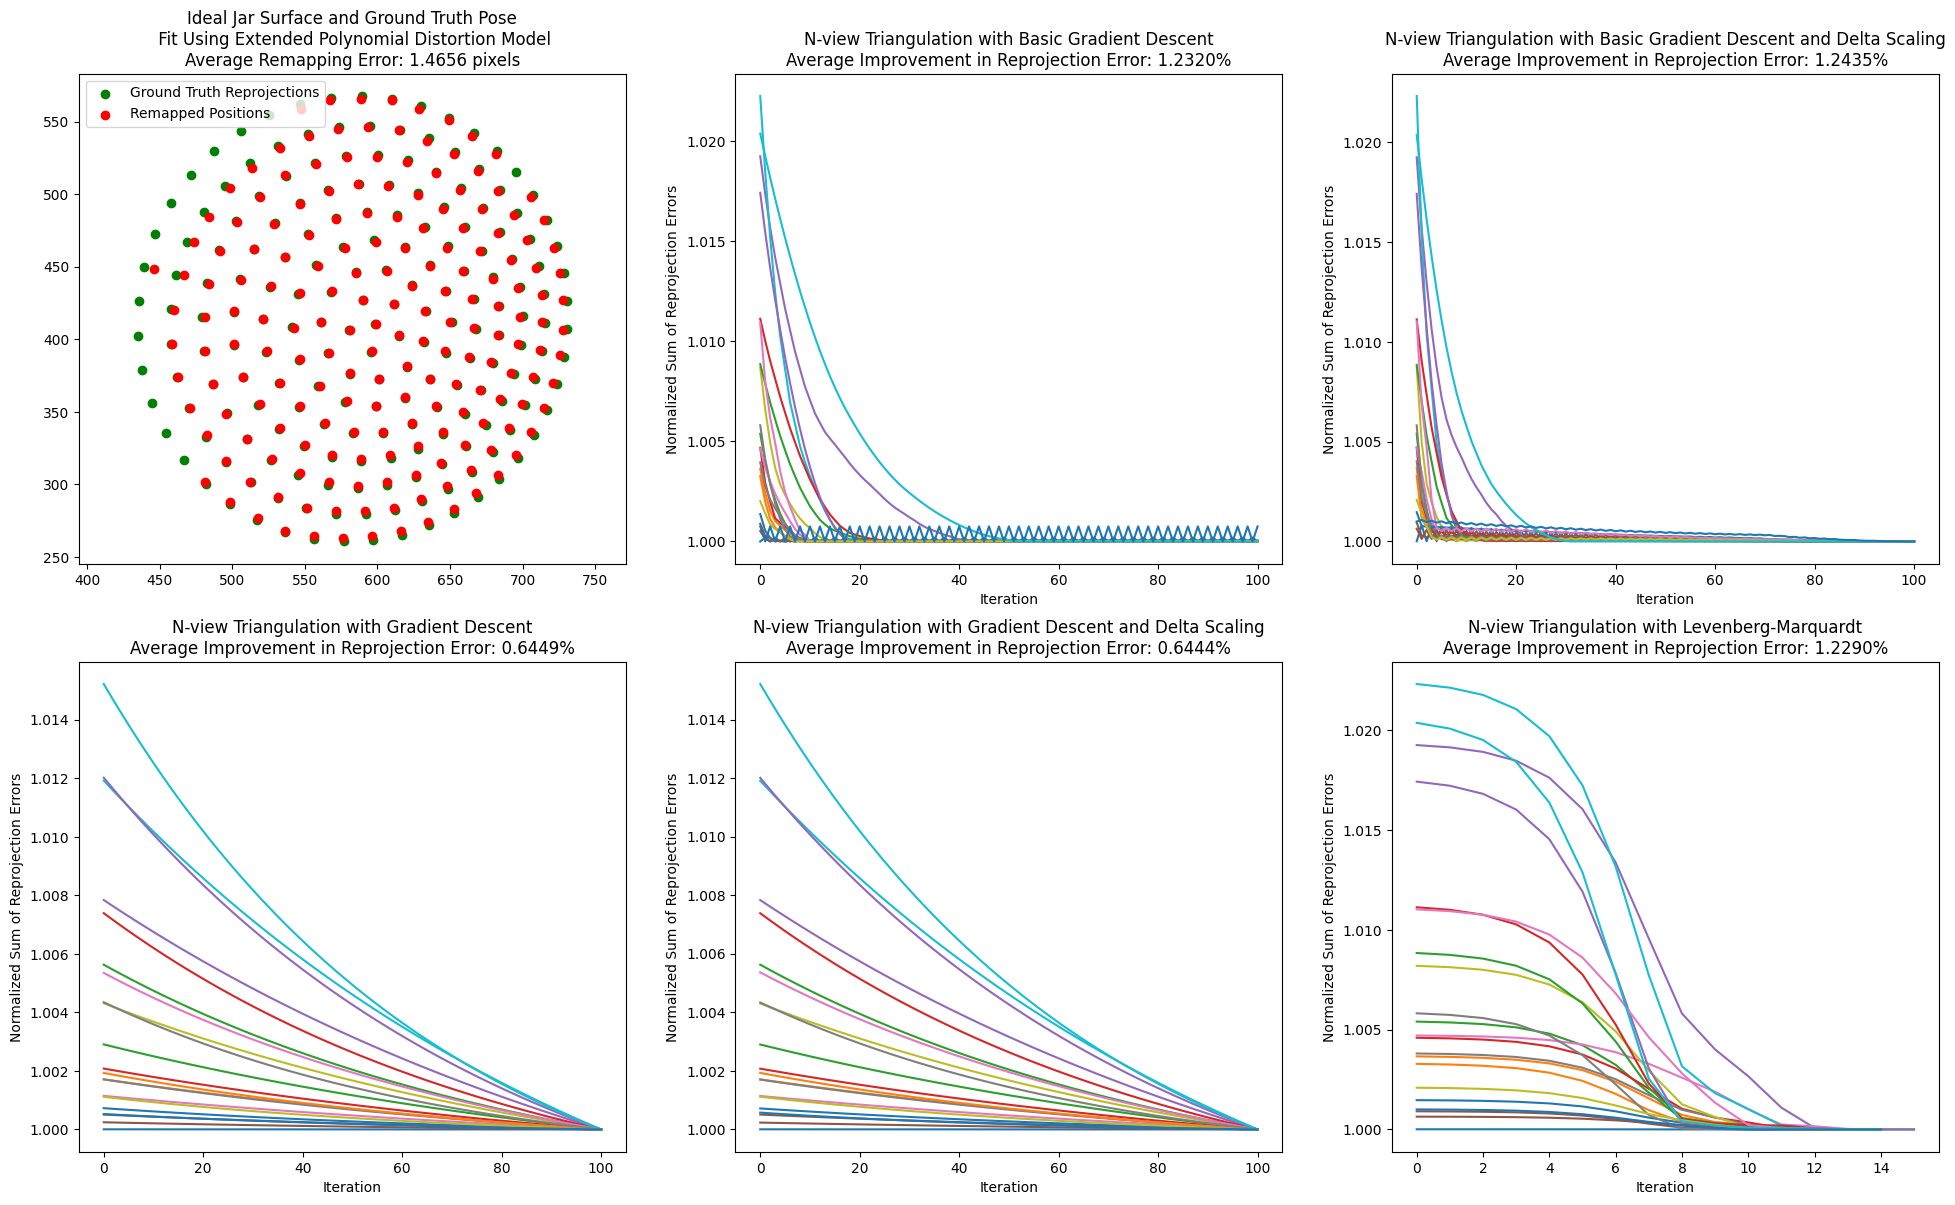
\includegraphics[width=\textwidth]{optimization_charts_for_ideal_jar_surface_and_ground_truth_pose.png}
    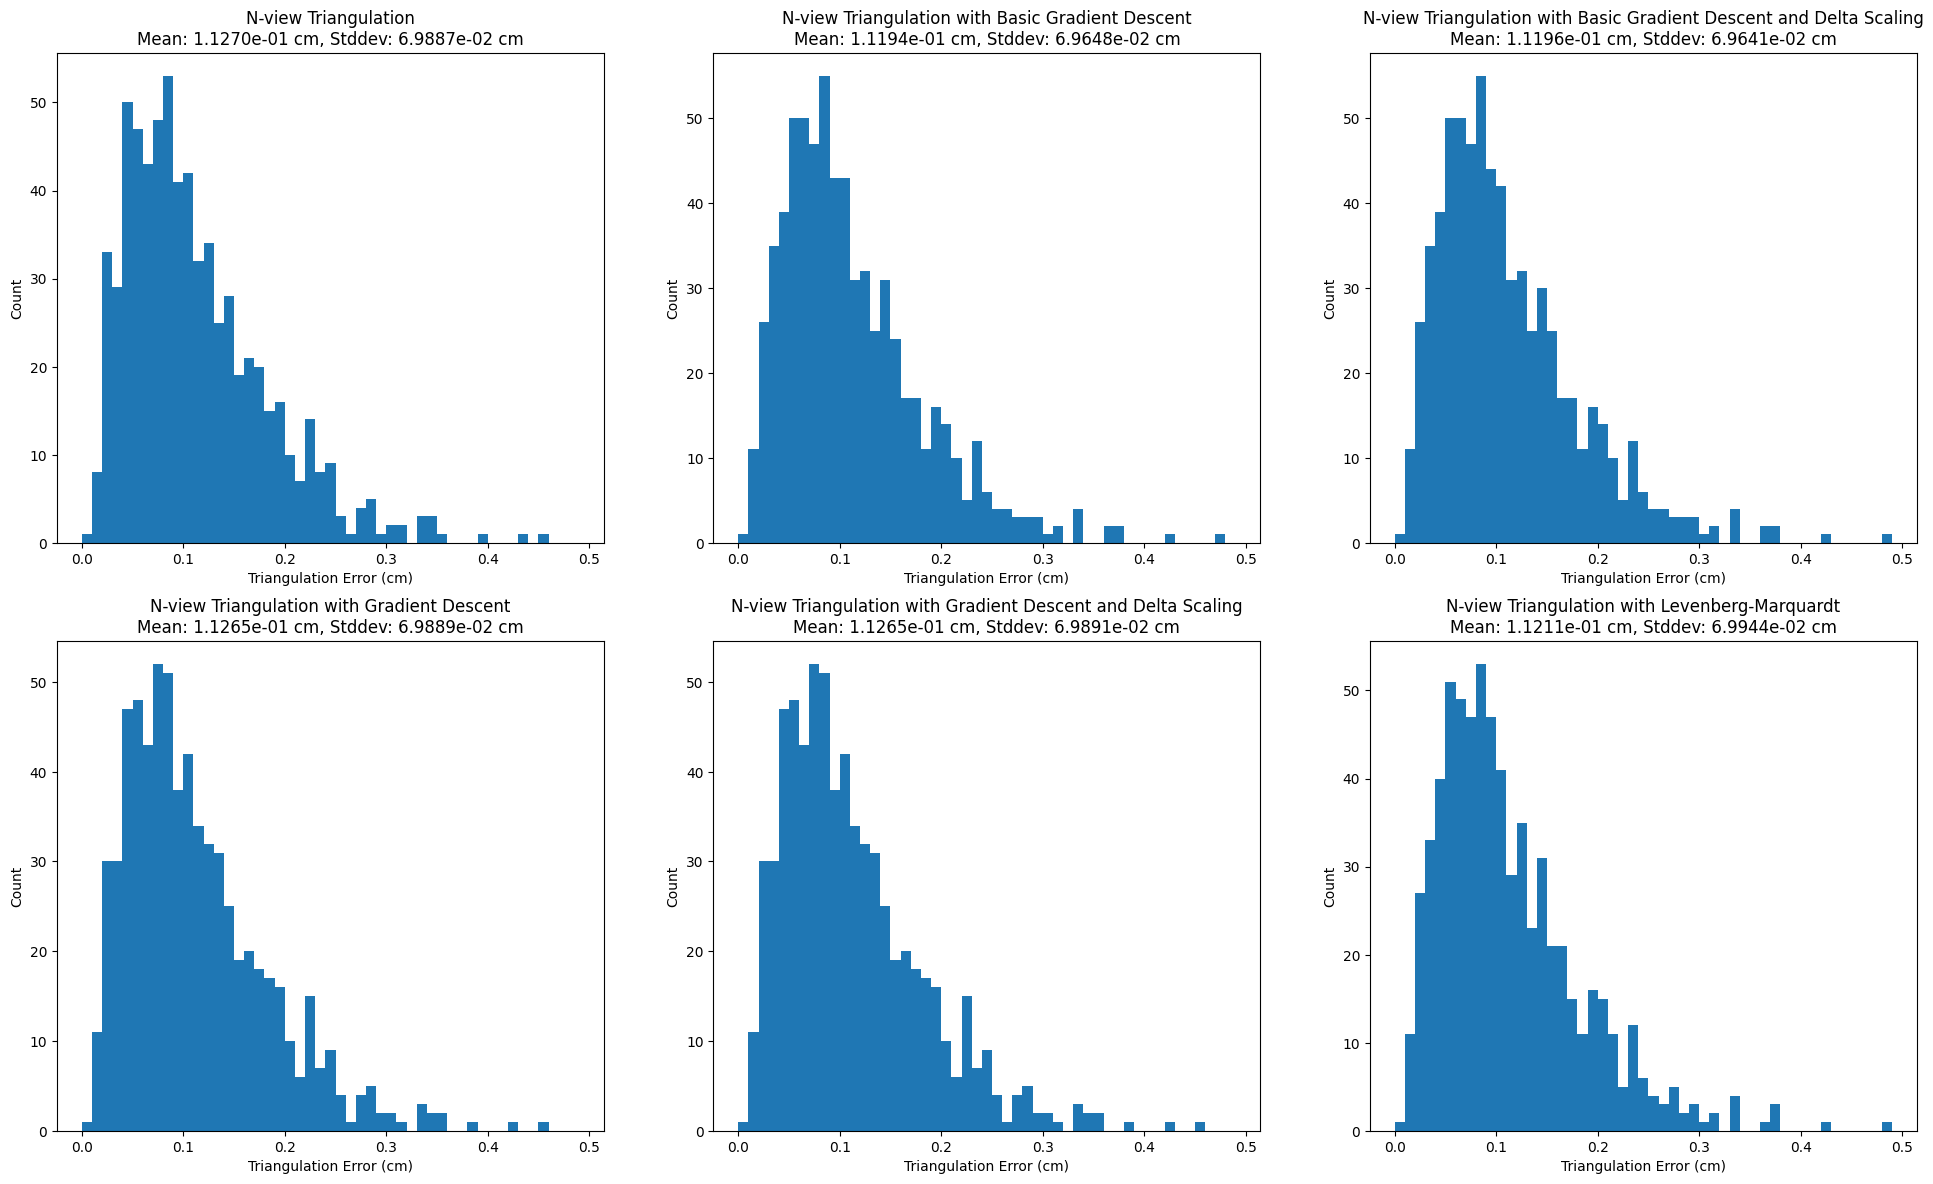
\includegraphics[width=\textwidth]{ideal_jar_surface_ground_truth_pose_triangulation_error_histograms.png}
    \caption{\textit{(Top left)} Pixel remapping for a simulated grid of points with an ideal jar surface and ground truth pose matrices. \textit{(Remaining plots in top two rows)} Normalized reprojection error plots for 20 grid points over 100 optimization iterations (except for LM), showing their convergence properties. \textit{(Bottom two rows)} Histograms showing distribution of triangulation errors after applying each optimization. Results show Basic GD with Delta Scaling has the best combination of convergence and accuracy improvement, although the improvements are minor.}
    \label{fig:optimization_charts_and_histograms_for_ideal_jar_surface_and_ground_truth_pose}
\end{figure}

\begin{figure}[h]
    \centering
    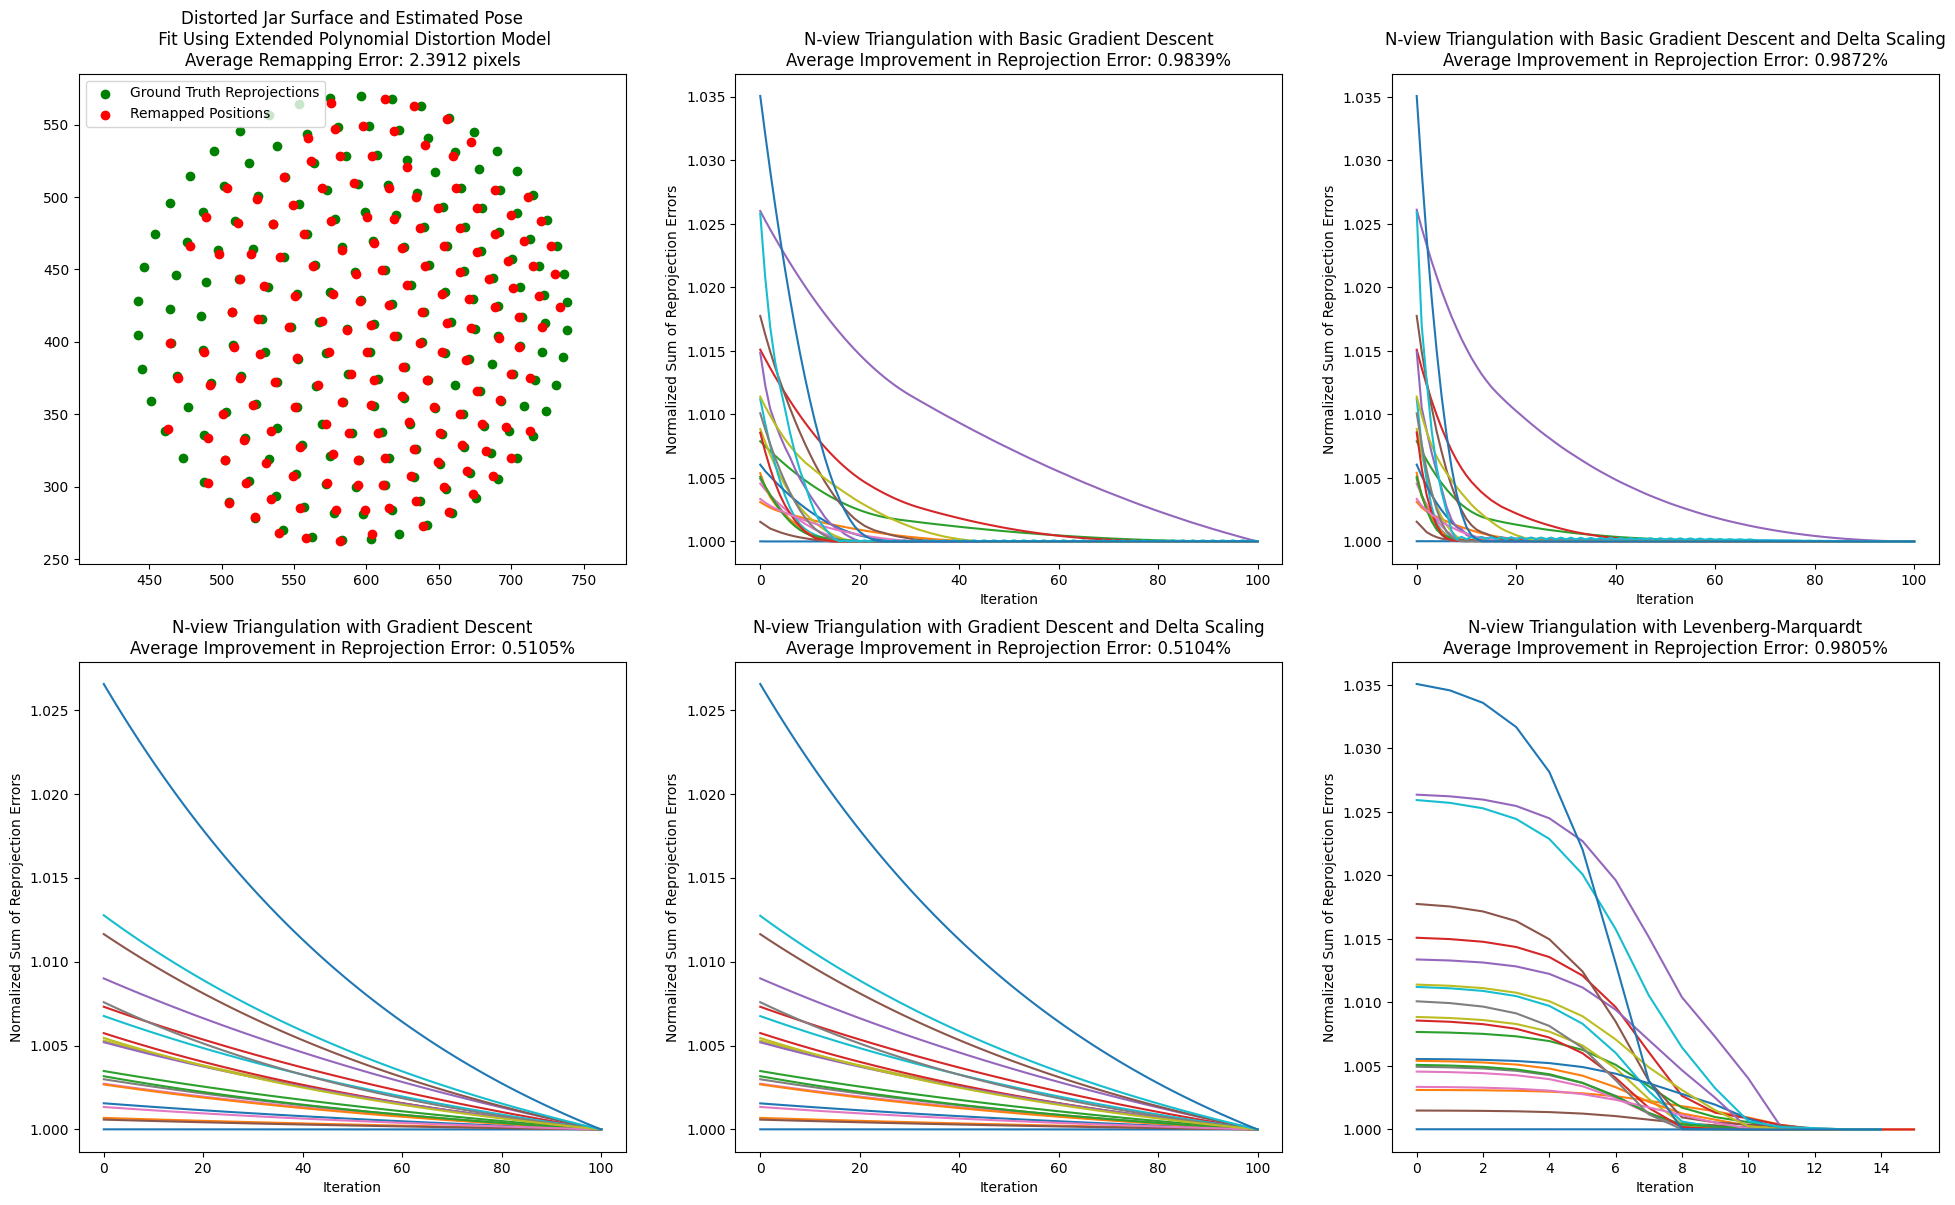
\includegraphics[width=\textwidth]{optimization_charts_for_distorted_jar_surface_and_estimated_pose.png}
    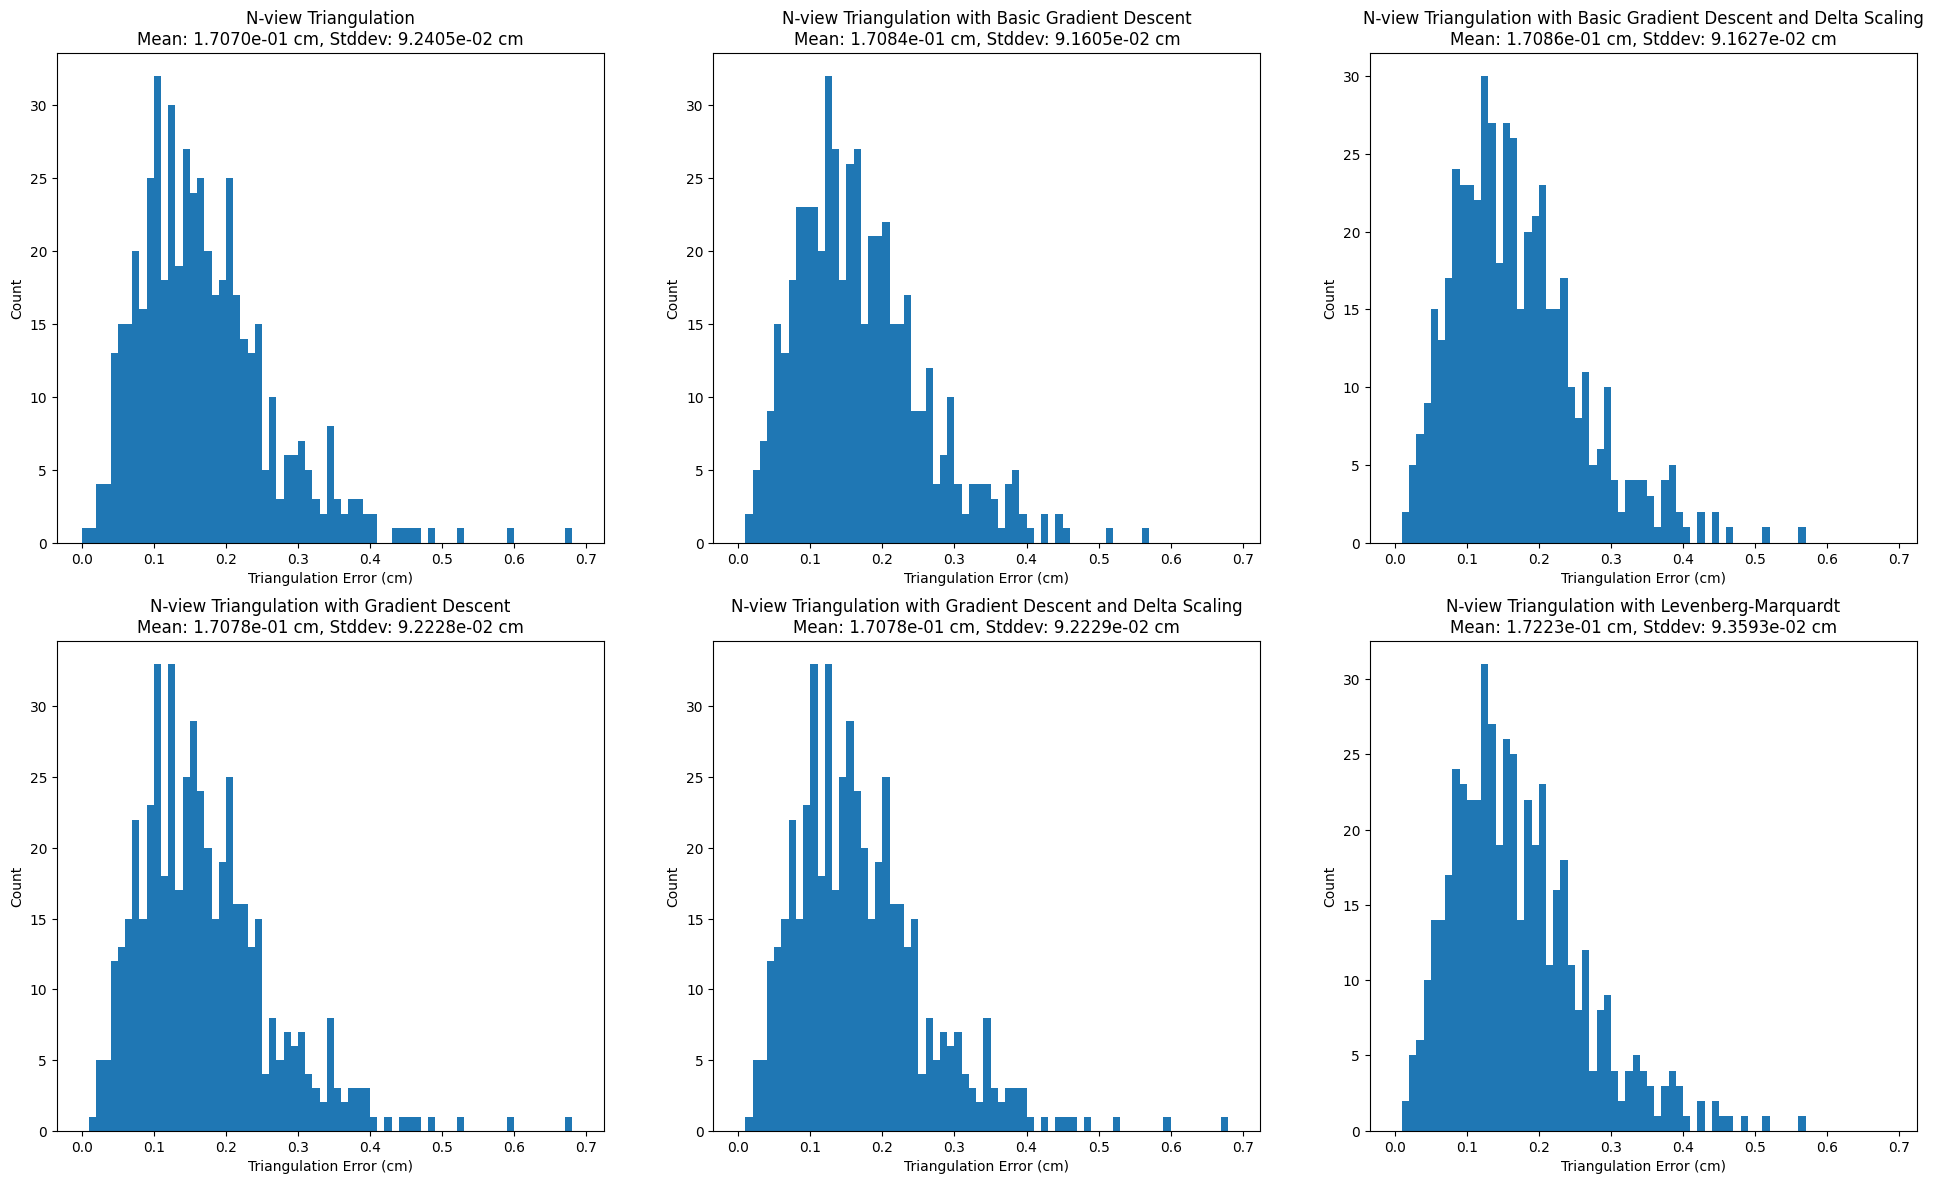
\includegraphics[width=\textwidth]{distorted_jar_surface_and_estimated_pose_triangulation_error_histograms.png}
    \caption{Same sub-plot layout as in figure \ref{fig:optimization_charts_and_histograms_for_ideal_jar_surface_and_ground_truth_pose} but now for a simulated grid of points with a distorted jar surface and estimated pose. Results show that optimizations applied to poorly localized pixel positions can \textit{reduce} triangulation accuracy.}
    \label{fig:optimization_charts_and_histograms_for_distorted_jar_surface_and_estimated_pose}
\end{figure}


\section{Summary of Error Contributions and Triangulation Priorities} \label{sec:summary_of_error_contributions}
From the tests presented in the previous sections, it is apparent that the accuracy of bubble localization is primarily determined by how close the ray origins and directions used for triangulation are to the ground truth for camera origins and the directions towards the bubble locations. Therefore, the factors that influence the ray origins and directions are the ones that have the largest impact on 3D localization error. 

Starting with ray directions, figure \ref{fig:pixel_remapping_error_on_triangulation_accuracy} showed that the relationship between pixel uncertainty and localization error can be modeled as a the following linear function: $y = 0.073606x - 1.43555\times 10^{-5}$ where $x$ is the error in pixels, and $y$ is the corresponding 3D localization error in centimeters. With this model, attaining sub-millimeter precision requires a maximum error of 1.36 pixels, and 2.72 pixels for sub 2-millimeter precision (assuming the camera poses are perfectly estimated). 

The error in pixel localization is influenced by the accuracy of the models used to fit the distortions caused by refractive surfaces in view of the camera sensors. This includes the distortion caused by the camera lenses. Therefore, having a good calibration for the camera distortion coefficients and camera matrix for each camera is critical, as camera distortions can easily add pixel errors in the range of 2 to 5 pixels in the center of the image (e.g. if the focal center is not aligned) up to 20+ pixels at the edges of the image. Coming up with better models for pixel remapping will also help, especially as the models presented in this paper do not handle the remapping of points close to the edges of the jars very well (see for instance, figure \ref{fig:extended_polynomial_fit_to_ideal_distorted_jar}). Errors in the IoRs of the fluids in the chamber (CF4 and LAr) also have the largest impact on pixel localization. As seen in figure $\ref{fig:effect_of_wrong_iors_on_remapping_and_localization}$, errors in the IoR used to determine the remapping functions of even just 1\% in either the IoR of CF4 or LAr can add up to 0.2 centimeter to the triangulation error (assuming no other sources of error). Finally, sub-pixel localization of bubbles \textit{can} help improve triangulation, however, the effects are insignificant if other sources of pixel error are larger.

Accurate pose estimation is also important as errors in the estimated camera positions and rotations have an approximately linear relationship with the triangulation error. As one might expect, the average error in camera location has a one-to-one correspondence with the average error in 3D point localizations (e.g., compare the y-axes of the left and right-most plots of figure \ref{fig:PnP_error_pixel_offset}). When estimating the pose using the PnP algorithm and the fiducial markers, having sub-pixel accuracy on the localization of the fiducial markers is extremely important, as even a maximum of a single pixel of error corresponds to an added triangulation error of about 1.8 pixels on average (see figure \ref{fig:PnP_error_pixel_offset}).

Finally, the triangulation algorithm used and the optimizations performed have a marginal impact on the overall localization. It is recommended to stick with N-view triangulation and use basic GD with $\delta$ scaling only if you have good pixel localization (e.g., within sub-pixel accuracy compared to the ground truth reprojections without refractive surfaces).

\subsection{Recommended Order for Computations}
This paper covered the computation for several values, often with the computation of a one value relying on other values. Therefore, in this section, we seek to clarify the order in which these values might be calculated. A corresponding flow chart of the steps can be found in figure \ref{fig:localization_flow_chart}.

First, the camera calibration of each camera which provides the camera matrix and distortion coefficients as in \S\ref{subsec:camera_calibration} should be completed using a calibration pattern as in \S\ref{subsubsec:zhang's_method_for_camera_calibration}.\footnote{Being able to perform camera calibration with a calibration pattern assumes that we have the cameras outside of the chamber. If it is not possible to remove these cameras from the chambers to perform calibration, using pre-existing estimates or alternative models such as in \S\ref{subsubsec:an_alternative_distortion_model} may be sufficient.} Additionally, the precise indices of refraction for the fluids at the operating temperatures and LED wavelengths (850 nm) should be determined.

Once the cameras are in the chambers, their poses can be estimated using the pixel positions of the fiducial markers from the calibrated camera images with no fluids in the chamber (so as to minimize the extra distortion caused by the magnification from the viewports when the chambers are filled with CF4). Then, using the estimated camera poses and pre-determined indices of refraction, the coefficients of the remapping functions for images taken when the chambers are filled with fluids can be determined using renders of the testing grid as in figure \ref{fig:testing_grid}.

Finally, when it is time to detect and triangulate bubbles, for each event where a bubble may have appeared, we can first background subtract the images of the bubbles, then search for bubbles in each difference image using the circle Hough transform as in \S\ref{subsec:circle_hough_transform}. Once all potential bubble locations are found, if more than one bubble exists in each image, we can first determine the corresponding bubble locations in each image using the undistorted bubble locations (as in \S\ref{subsec:corresponding_bubbles}). Then we run n-view triangulation using those undistorted pixel locations and the corresponding camera and pose matrices. Optionally, we can optimize the result by running basic gradient descent with delta scaling on the estimated bubble location and using the calculated bubble positions determined using the Hough transform. 


\begin{sidewaysfigure}
    \centering
    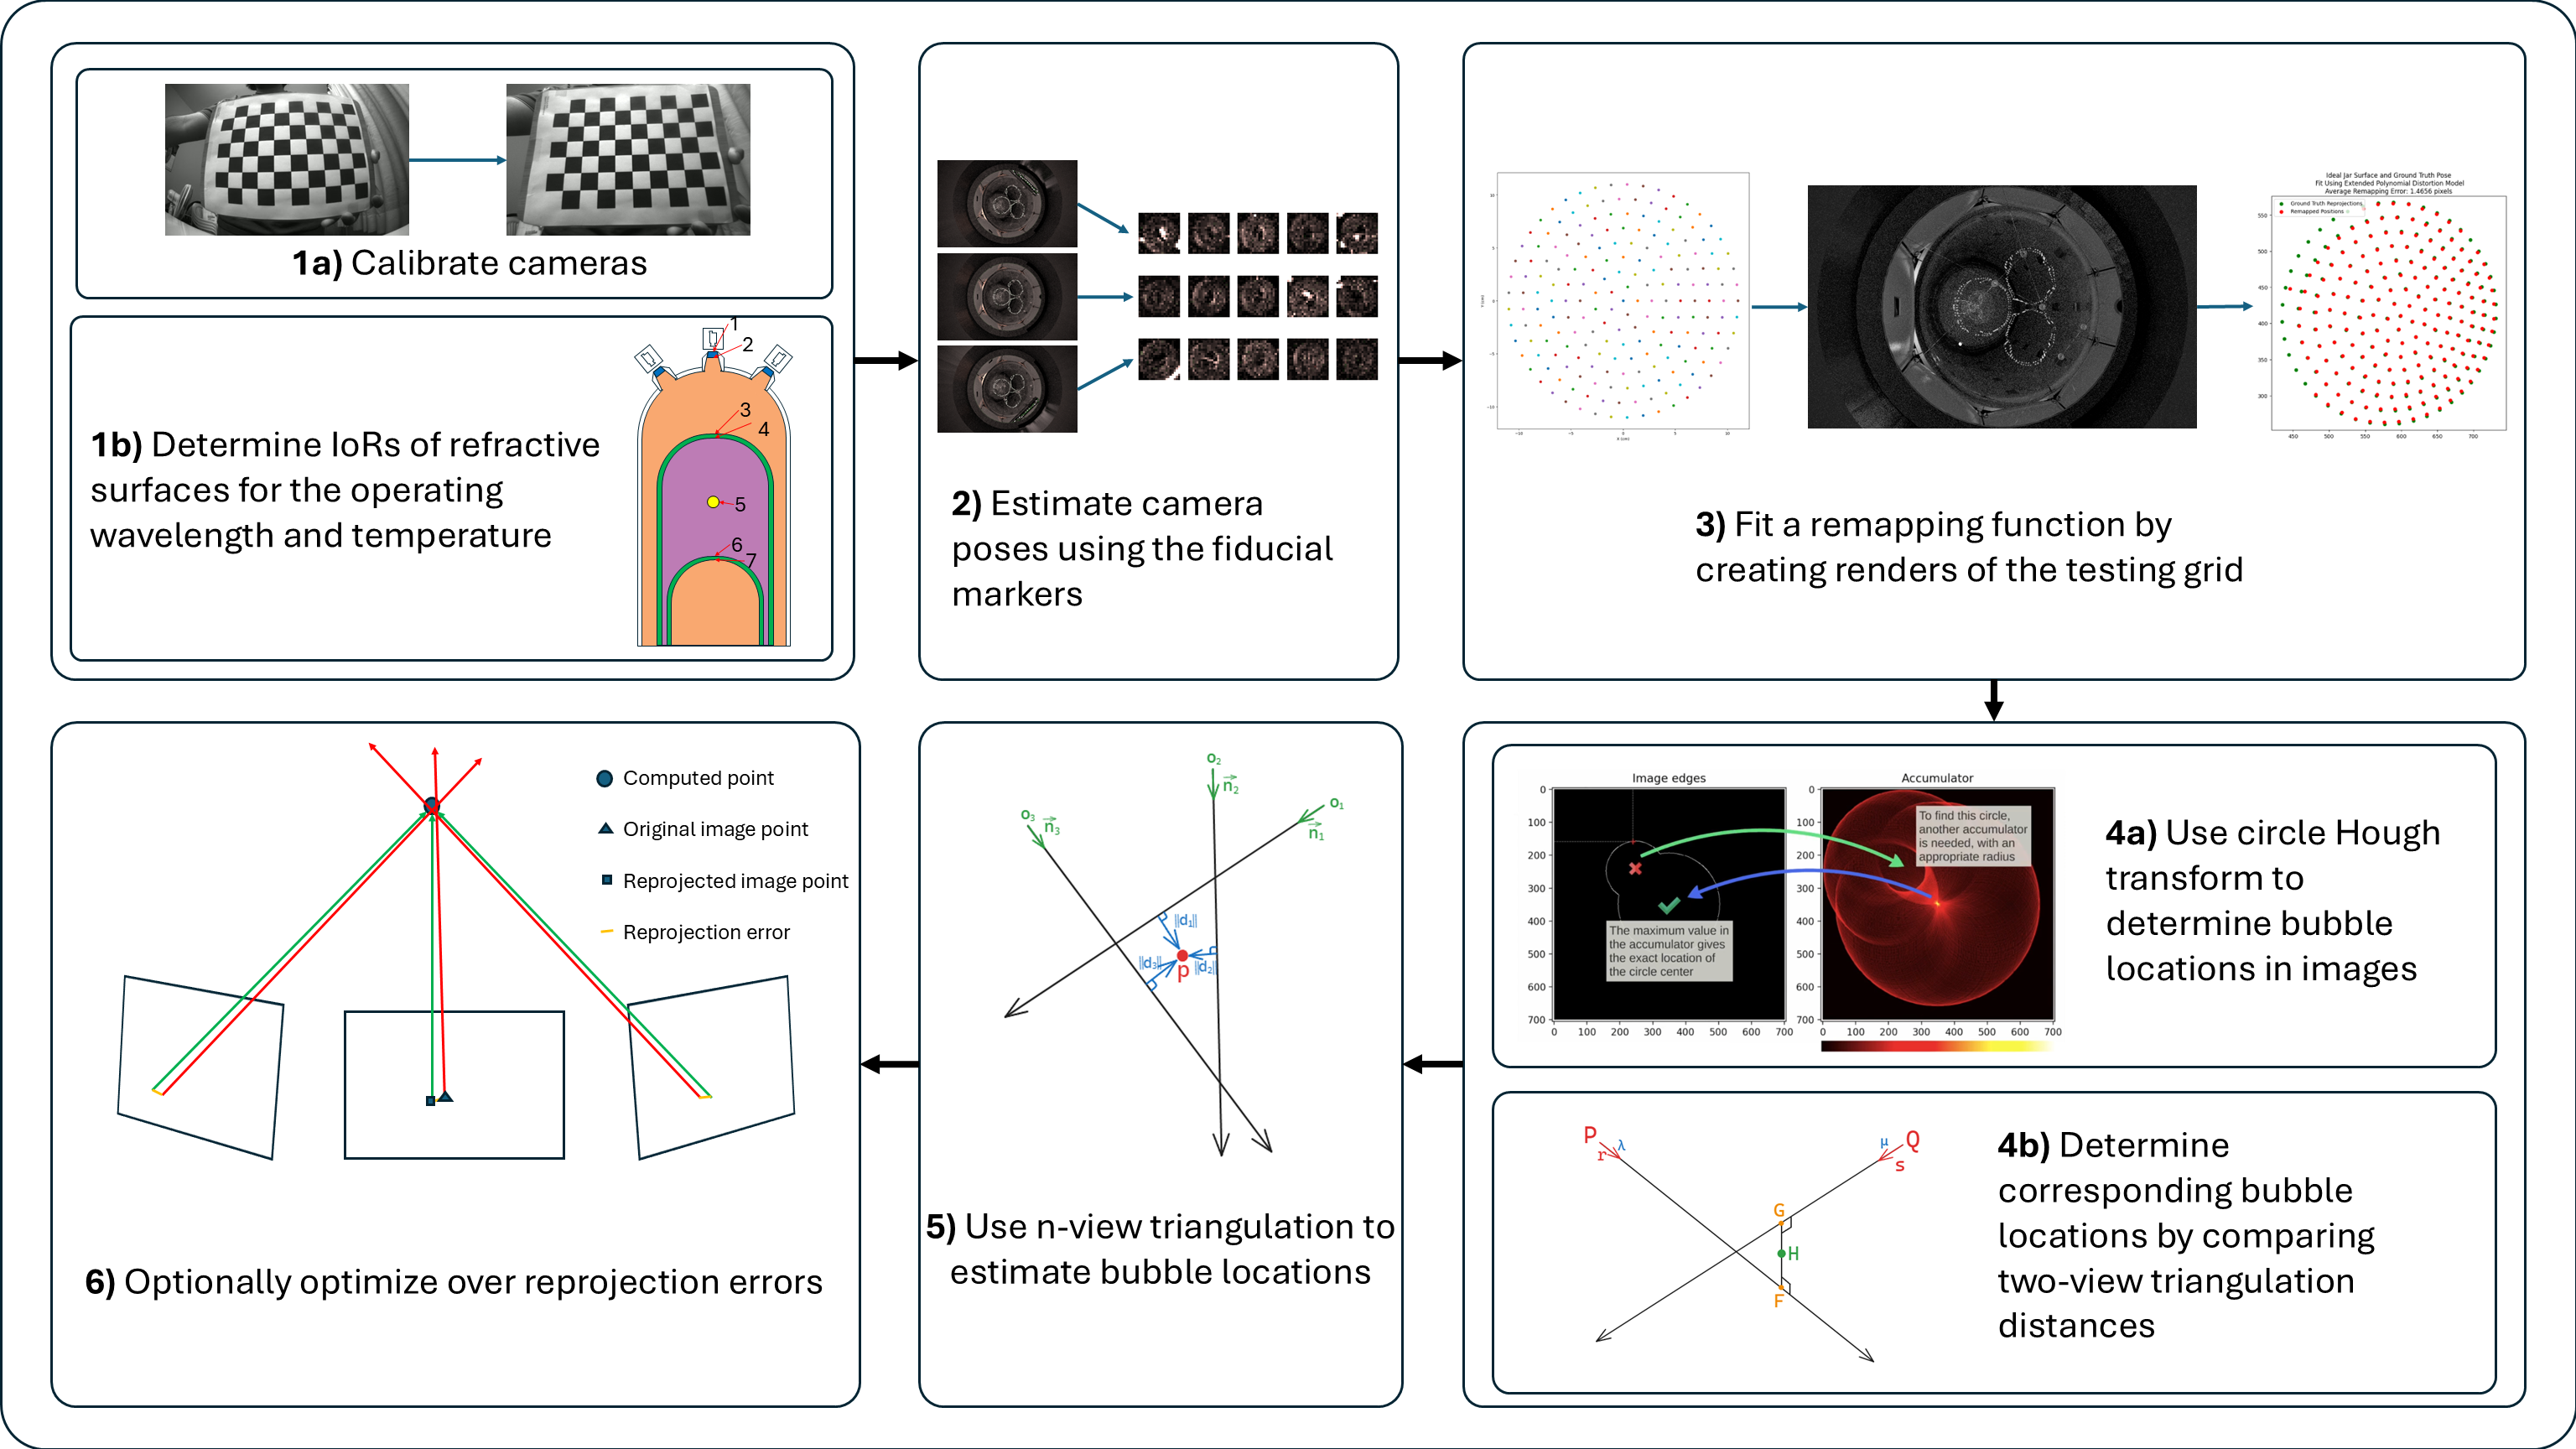
\includegraphics[width=\linewidth]{localization_flow_chart_2.png}
    \caption{A flow chart of the order in which triangulation steps can be completed.}
    \label{fig:localization_flow_chart}
\end{sidewaysfigure}


\section{Conclusion} \label{sec:conclusion}
This paper discusses methods for bubble detection and triangulation for the SBC chambers and the factors that most-influence the triangulation accuracy of bubbles. In conjunction, the paper also discusses how the research oriented renderer, Mitsuba, was used to test the methods and provide simulated images that mimic the true images of the chambers. 

The factors that most influence triangulation accuracy are the ones which affect the ray origins and directions used in the triangulation algorithms. Those factors are, in order of their sensitivity to influence the errors: the estimated pose of the camera, errors in the indices of refraction of the fluids used to fit the remapping functions, the distortions caused by the camera lenses, the ability of the remapping functions to adequately account for the distortions introduced by the viewport magnification and jar surfaces, and the sub-pixel estimate of the 2D bubble locations. Consequently, we suggest focusing on getting precise pose measurements, precisely determining the indices of refraction for the liquids in the chamber, getting accurate camera calibrations, and finding and fitting a good model for remapping distortions introduced by magnification through the viewport and distortions from the outer jar.

\subsection{Future Work} \label{subsec:future_work}
The main area of improvement that still remains with regards to bubble localization is determining a better model for remapping pixel positions and dealing with jar surface distortions. One important factor in fitting accurate remapping functions is having a good model of the jar surface. Mitsuba was originally chosen as the renderer because of its ability to do \textit{inverse rendering}, i.e., update a scene to match existing images. The hope was to use Mitsuba to model the jar surface distortions by comparing the rendered images to the true images of the chamber and optimize the jar surface using the reflections of the LEDs. However, that proved too difficult, at least within the time span of this paper, to get working properly. 

For future reference, the jar surface can be estimated as being radially symmetric, so the jar surface distortions can be modeled as a Fourier series whose coefficients can be used as a displacement map for the vertices of the jar's top surfaces (similar to how the distortion map in figure \ref{fig:distorted_jars_renders} was used to displace vertices of the jar surfaces along their normals). In theory then, determining the jar surface distortions should be as simple as determining the coefficients of the Fourier series which, when applied as a distortion map to the jar surface, causes the reflections of the LED rings to match the reflections seen in the true images. Getting this to work in practice, however, is another story.

Additionally, a better bubble detection algorithm needs to be devised. Even within the rendered images where the bubbles were represented as light sources, the Hough transform was unable to detect the `bubbles' because they were distorted to the point of no longer being circles (e.g., see figure \ref{fig:extended_polynomial_fit_to_ideal_distorted_jar}). Alternatives may include methods such as \textit{blob detection}, or it may even be the case that background subtraction on its own, combined with a threshold and `center of mass' method as briefly discussed in \S\ref{sec:bubble_detection} may be enough. 

% \appendix
% \section{Setting Up Mitsuba}
% \section{Editing the Scene}

\newpage
\singlespacing
\nocite{*} % add all citations to the bibliography even if they are not manually cited in the paper
\printbibliography

\end{document}
